 \documentclass[oneside,11pt]{article}


\usepackage{soul}
\usepackage{natbib}
\usepackage{hyperref}
\usepackage{bookmark}
\usepackage{graphicx}             
\graphicspath{{./Figuras/}}

\usepackage{makecell}
\usepackage[margin=1in]{geometry}
\usepackage{float}                
\usepackage{amsmath}
\usepackage{amscd}
\usepackage{amsfonts}
\usepackage{amssymb}
\usepackage{bbm}
\usepackage{booktabs}
\usepackage{nameref}
\usepackage{multirow}
\usepackage[nokeyprefix]{refstyle}
\usepackage{rotating}
\usepackage{threeparttable}
\usepackage{afterpage}
\usepackage{lscape}
\usepackage{enumerate}
\usepackage{caption}
\usepackage{subcaption}
\usepackage{epstopdf}
\usepackage{setspace}
\usepackage{svg}
\usepackage{dsfont}
\usepackage{amsthm}
\usepackage{tocloft}
\usepackage{etoc}
\usepackage{lmodern}
\usepackage{bm}

\epstopdfDeclareGraphicsRule{.tiff}{png}{.png}{convert #1 \OutputFile}
\AppendGraphicsExtensions{.tiff}

\epstopdfDeclareGraphicsRule{.tif}{png}{.png}{convert #1 \OutputFile}
\AppendGraphicsExtensions{.tif}

\usepackage{tikz}
\usetikzlibrary{shapes.geometric, arrows}
\usetikzlibrary{calc}
\usetikzlibrary{matrix}

\tikzset{ 
    table/.style={
        matrix of nodes,
        row sep=-\pgflinewidth,
        column sep=-\pgflinewidth,
        nodes={
            rectangle,
            draw=black,
            align=center
        },
        minimum height=1.5em,
        text depth=0.5ex,
        text height=2ex,
        nodes in empty cells,
%%
        every even row/.style={
            nodes={fill=gray!20}
        },
        column 1/.style={
            nodes={text width=2em,font=\bfseries}
        },
        row 1/.style={
            nodes={
                fill=black,
                text=white,
                font=\bfseries
            }
        }
    }
}


\usepackage{colortbl}

\newtheorem{theorem}{Theorem}
\newtheorem{claim}[theorem]{Claim}
\newtheorem{prop}[theorem]{Proposition} 
\newtheorem{cor}[theorem]{Corollary} 

\DeclareRobustCommand{\hlgr}[1]{{\sethlcolor{green}\hl{#1}}}


\usepackage{comment}
%para esconder columnas en tablas (enrique)
\usepackage{array}
\newcolumntype{H}{>{\setbox0=\hbox\bgroup}c<{\egroup}@{}}
\linespread{1.25}

\newcommand{\wh}{\widehat}
\usepackage{anyfontsize}

\usepackage[linesnumbered,vlined,ruled,commentsnumbered]{algorithm2e}

\DontPrintSemicolon
\newcommand{\To}{\mbox{\upshape\bfseries to}}
%%% HELPER CODE FOR DEALING WITH EXTERNAL REFERENCES
\usepackage{xr}
\makeatletter
\newcommand*{\addFileDependency}[1]{
  \typeout{(#1)}
  \@addtofilelist{#1}
  \IfFileExists{#1}{}{\typeout{No file #1.}}
}
\makeatother


\newcommand*{\myexternaldocument}[1]{
    \externaldocument{#1}
    \addFileDependency{#1.tex}
    \addFileDependency{#1.aux}
}

%\myexternaldocument{OA}

%%%%%%%%%%%%%%%%%%%%%%%%%%%%%%%% DOCUMENT
\begin{document}


\title{The limits of self-commitment and private paternalism \thanks{We want to thank Mauricio Romero and Anett John for advice and encouragement. Ricardo Olivares, Gerardo Melendez, and Alonso de Gortari provided excellent research assistance and Erick Molina helped with formatting. Jose Maria Barrero, Andrei Gomberg, Emilio Gutierrez, David Laibson, Aprajit Mahajan, Matt Rabin, Charlie Sprenger, and seminar participants at ITAM provided valuable feedback.}}
\author{Craig McIntosh \and Isaac Meza \and Joyce Sadka \and Enrique Seira   \thanks{Seira: ITAM, enrique.seira@gmail.com (corresponding author); Meza: University of California at Berkeley, isaac.meza@berkeley.edu; Sadka: ITAM, jsadka@itam.mx} }
\date{This draft:  \today \\[2 cm]}

%\vspace{.5in}


\maketitle
\thispagestyle{empty}
\begin{abstract}

%Many firms provide commitment devices that restrict individuals' choice, but shroud this. Shrouding suggests low demand for commitment. We show that private paternalism is beneficial in the pawnbroker context we study. 

In the context of pawnbroker lending, we show that forcing people into commitment contracts with financial penalties for not paying on time \textit{decreases} their (fee-including) financial cost by 9.4\%, increases the likelihood of recovering their pawn by 26\%, and increases the likelihood of repeat business by almost 100\%. Using machine learning methods for estimating heterogeneous treatment effects, we find that more than {70}\% clients would reduce their financing cost with the commitment contract, however only 10\% choose it. Those that \textit{don't} choose it are predicted to be the ones who would benefit more. Relying on personal promises instead of fees as commitment triples take-up but has no effects on outcomes.

%and one of the most understudied. In our context more than on half of borrowers default and lose their pawn and whatever they have paid towards recovering it. Compared to the status quo pay-at-anytime 3-month contracts, forcing borrowers to pay monthly and charge a penalty if they didn't --i.e. a commitment contract-- increased recovery of pawn by about 30\% and financial costs by 10\%. However when offered a choice between the two contracts only 10\% took the monthly payment one. A pecuniary commitment seems necessary. In an alternative arm, we made them promise to pay but removed the pecuniary penalty. This increased take up to 31\%, but had zero effect on financing cost or default. The forcing contract may be better than choice for naive present biased consumers.

\end{abstract}

\vspace{.3in}

\textbf{Keywords: } Private paternalism, choice, present bias, naivete, overconfidence, commitment, heterogeneous treatment effects.

\textbf{JEL codes:} G41, C93, O16, G21

\newpage

\pagenumbering{arabic}
\etocdepthtag.toc{mtchapter}
\etocsettagdepth{mtchapter}{subsection}
\etocsettagdepth{mtappendix}{none}


%NO MORAL HAZARD IN THE CONTRACT SINCE FULLY COLLATERALIZED
%DOUBLE FAILURE: DEMAND LOW, AND DOES NOT WORK BY PEOPLE WHO TAKE IT.
%PENALIZES THEM EVEN MORE ON SOMETHING THEY WERE ALREADY PENALIZED 
%PROPENSITY TO CHOSE.
%PULLING PUNISHMENT FORWARD --CHARGING RIGHT WHEN I MESS UP.
%MAYBE ONLY IMPATIENT AND NAIVE END IN PAWNSHOPS
%1) SELECT A RANDOM SAMPLE OF NEIGHBORHOODS, EXTERNAL VALIDITY, THE ONES THEY GO ARE NAIF AND
%HYPERBOLIC
%2) ASK TO CHOSE AMONG ALL CONTRACTS
%3) CLASSIFY SOPHISTICATION AT BASELINE
%4) HOW TO GET AT SHOCKS.  --BUT DOES NOT SQUARE WITH WHY CHARGING THEM FEES WORKE.
%do shocks vary across strata, predict shocks.
%DEEP BEHAVIORAL PAPER -- CAN WE REALLY PREDICT?



% \section{Introduction}

Many institutions ---firms, schools, financial contracts--- restrict choice using built-in commitment mechanisms which help workers, students, borrowers overcome self-control problems. For instance, ``[mortgages restrict choice] with a fixed repayment stream and mandatory principal repayment'' \citep{Laibson2018}.\footnote{\cite{Laibson2018} also mentions that ``Firms do limit their workers' freedom with intermediate deadlines, progress reports, production targets'', and schools with ``pop quizzes, classroom attendance requirements, cold calling, graded problem sets, deadlines''.} At the same time  these same firms shroud and don't market these commitment features, presumably because students, workers and borrowers don't welcome these restrictions. \cite{Laibson2018} argues that this presents an important puzzle: clients that would benefit from commitment underestimate its value and thus have low demand for it. In such a case private paternalism may be beneficial.\footnote{Laibson defines paternalism as a policy that advances an individual's interests by restricting his or her freedom, and private paternalism as paternalism implemented by private institutions. %In this paper we will study the effect of restricting freedom of contract choice on two outcomes: pawn recovery and financing cost, not overall welfare.
We want to clarify that we are using the word ``paternalism'' in a restricted sense, meaning only that a large majority of clients would incur in lower financial costs from being forced into installment contracts instead of letting them choose. We are not making claims about overall welfare which is a slippery concept if we take into account the possibility of biased beliefs and preferences.} 

This paper studies the benefits of restricting choice in the context of pawnbroker lending. Pawn loans are one of the oldest, most understudied, and most prevalent forms of borrowing. There are more than 11,000 pawn shops across the US, with 30 million clients and \$14 billion yearly revenues. In China it is a 43 billion dollar industry.\footnote{\url{https://tinyurl.com/ybm56dpe}, \url{https://tinyurl.com/y9zdcgws}, \url{https://tinyurl.com/y59ptdam}.} Our partner pawn lender (henceforth Lender $P$) alone served more than 1 million clients in the last 3 years with more than 4 million contracts. The key characteristic of pawn loans is that the borrower leaves personal property (a pawn) as collateral in exchange for an immediate cash loan of a smaller value. In our case Lender $P$ only accepts gold jewelry as collateral and approves all pawns, giving cash the equivalent of 70\% of the pawn's appraised value. The contract stipulates a 7\% monthly interest rate charged daily, a loan term of 90 days, and the flexibility to pay back the loan at anytime before the loan is due. In spite of this flexibility ---or perhaps because of it--- 60\% of clients lose their pawn\footnote{In the US default is also high at 15\% (\url{https://tinyurl.com/yc2x5bjf}).}, and among those that recover it almost all of them pay in the days just before the loan elapses.

% About 85\% of borrower lose their pawn\footnote{https://nationalpawnbrokers.org/2017/06/19/pawnbroking-around-the-world/}

%different prices: https://priceonomics.com/the-economics-of-pawn-shops/

% pawnshops help the poor https://tinyurl.com/y9qr43j8
%, with annual percentage rates above or close to 200\%.  

% Limite statustics and knowledge of pawnshops. World bank mentions them in passing: https://tinyurl.com/ydgob8pv

%Borrowers typically turn to these loans when in desperate need to pay for an emergency. The vulnerability of these borrowers has sparked regulator's interest.\footnote{In 2013 Mexico's Consumer Protection Bureau (Profeco) is concerned about abuse. It forced Pawnshops to be more transparent in their pricing, register their contracts with them and issued regulation to protect clients. Congress has enacted laws in this regard. \url{http://www.diputados.gob.mx/LeyesBiblio/ref/lfpc.htm}.} One concern is that borrowers selecting into these loans may exhibit particularly strong behavioral biases. 
%Using a survey conducted by us in branches of Lender $P$, we indeed document some evidence consistent with these concerns: while pawnshop clients predict they will recover their pawn with 93\% probability on average, in reality only 40\% of them do, suggesting naivete. 
%Even conditional on paying a positive amount towards pawn recovery, 53\% lose their pawn and their payment. In our survey 69\% report self-control problems saying they often fall into temptation spending. %, but only gr{15\%} show inter-temporal inconsistencies in a classical present-bias question, a similar number to \cite{Ashaf}. %and {19\%} do not normally budget monthly expenses. 
%While this is suggestive of a present bias problem or overconfidence to save and pay, at the same time our subjects are experienced and not wholly uneducated, 66\% have completed at least high school and 90\% have pawned before. %and {38\%} have participated in a Rosca.

We implemented a large randomized control trial with close to 10,000 pawnshop clients in 6 branches of Lender $P$ in Mexico City. We answer five main questions using this experiment. First, would clients benefit  ---in terms of recovering their pawn and in terms of incurring in lower financing costs---  from having a frequent (monthly) payment commitment contract \textit{forced} on them, instead of the current 3-month pay-when-you-want contract? That is, we are asking whether \textit{charging} them a 2\% late payment fee for not paying a monthly installment on time can actually \textit{decrease} total (fee-inclusive) financing cost. Second, would there be demand for such an installment contract vis-a-vis the status quo one if given the choice? Note that any payment profile implemented in the commitment contract can be replicated by the borrower under the status quo contract, but the former provides commitment. Third, would clients who benefit from commitment the most (e.g. the present biased or overconfident) demand it more? Fourth, are late payment fees key to provide commitment or would a non-pecuniary but salient personal promise to pay provide a cost-reducing mix of commitment vs flexibility? Promises change behavior significantly in laboratory settings, but we know little about their effect in natural environments.\footnote{%Some papers in this space are \cite{PromisesPartnerships}, \cite{Vanberg}, \cite{Belot2010}, \cite{WhyDoPromises}, \cite{FurtherPromises}, \cite{Ismayilov2017}. 
There is some actual policy around using promises for loans: the government Mexico has created a program called ``Loans on your word'' for uncollateralized borrowing (\url{http://tiny.cc/yfmnmz}), but unfortunately there is little information about them.} Finally, is \textit{giving choice} among contracts better than forcing clients into payment-commitment contracts in terms of minimizing financing costs incurred and the likelihood of recovering their pawn? Or on the contrary, is it better to force the installment contract 
paternalistically?

The experiment involved 5 arms, with randomization happening at the branch-day level. It is described in detail in Section \ref{Experiment}. Here let us briefly explain the main 3 arms. The first one involves a group of clients that were given only the status quo flexible payments contract (henceforth the \textit{status-quo forcing group}). The second arm (\textit{fee-forcing group}) was given a monthly payment commitment contract, which stipulated that clients had to pay 1/3 of their loan plus accumulated interest in each of the 3 months of the term length. Failing to do this would result in a fee of 2\% of the amount due that month. A third group (\textit{Fee-choice group}) gave clients a choice between these two contracts. 

Results are striking. First, we find that forcing clients into frequent payment commitment contracts causes them on average to save on financing cost and to recover their pawn more. The effects are large: financing cost decreases by 9.4\% on average (from \$3157 to \$2860 MXN), while the likelihood of recovering their pawn increases by 26\% (from 43\% to 55\%). Results are robust qualitatively to including transport costs of going to the branch plus losing a day's wage for each visit. Importantly, the benefits are distributed broadly: almost the whole distribution of treatment effects shows cost savings; however those most economically vulnerable, and notably, those we classify as overconfident, experience larger gains. %The commitment contract also causes payments to start 8 days earlier and be 16\% more frequent, compared to the control group. 
Treatment effects are concentrated in the intensive margin as treatment does not affect the fraction of clients who pay a positive amount towards pawn recovery. That is, the fee-commitment contract induces people who would otherwise pay something towards recovery, to pay more and faster and thus recover their pawn more at a cheaper financial cost. Finally, borrowers assigned to the forced fee-commitment contract are 5 percentage points (100\% of the mean) more likely than the control group to ask for another loan in the future, suggesting that they liked the commitment contract after experiencing it.

%From this first comparison we conclude that penalizing borrowers for delinquency in a contract which has already has large penalties from default actually helps borrowers. In fact, we find that borrowers assigned to the forced fee-commitment contract are 5pp more likely to be repeat costumers, suggesting that they themselves liked the the commitment contract more after experiencing it.\footnote{As it is well known, \textit{naivete} facilitates their exploitation by firms. \cite{Laibson2018} conjectures that this exploitation may be limited if consumers use experienced utility to choose among firms or contracts.}

Second, in spite of these estimated benefits for almost all clients, actual demand for the fee-commitment contract is low. Only 10\% of the group offered a choice between the monthly payment fee-commitment contract and the status-quo one chose the former. This is not likely driven by misunderstanding the (already simple) contract.\footnote{We posted two project assistants in each of the experimental branches every day for all branch opening hours to carefully explain the contracts; material was developed to explain the differences among the two contracts, and subjects spelled back to our team the loan differences. Furthermore take up is systematically predicted by baseline covariates, making it less likely that these are just random mistakes.} We show further that clients that most benefit from the contract (those who are overconfident about recovering) are \textit{less} likely to demand it, echoing a result by \cite{Sprenger} for grocery purchases and \cite{Walters} for schools. %is Low demand for commitment is consistent with a large literature (\cite{Laibson2015}, \cite{Laibson2018}, \cite{John}, \cite{Ted}, \cite{Rabin2018}). 
%\footnote{\cite{Alcohol} and \cite{Kremer} are some of the few instances of high demand for commitment. \cite{Alcohol} speculates that this difference may be explained by their subjects having more experience with their self control problem. Close to ninety percent of our subjects claim to have pawned before. We find that experience does not predict positive take up in our sample.} 
%\cite{Laibson2015} shows that the lost flexibility resulting from a commitment contract can severely limit take-up when agents are naive about their self control, even though commitment could be welfare improving for them. 
Owing to this low take-up, we estimate zero average treatment effects of the \textit{fee-choice} arm on financial cost and on pawn recovery throughout the quantile distribution.

 %Using boosting we can predict who takes up with 92\% accuracy. This fact shows that the choice among contracts is not purely random.

Third, combining the forcing and the choice arms ---a unique feature of our experiment--- allows us to estimate the counterfactuals to answer the question of how much money is left on the table by giving choice to clients. We calculate that about {80}\% of clients in the fee-choice group chose contracts that induced \textit{higher} financial cost. On average they spend an extra \${238} MXN, close to {11}\% of the average loan value. In particular {92}\% of those that chose the status-quo contract would have been better in the fee-commitment contract, while only {8}\% of those who chose the fee-commitment contract would have been better in the status-quo one. This suggests that forcing clients into commitment contacts ---private paternalism--- may be beneficial for the overwhelming majority of clients. After seeing our results Lender $P$ introduced frequent payment contracts in their loans portfolio.

Inspired by a significant lab experiment literature on the effects of promises on behavior, and by research showing that a small fee could drastically reduce demand for commitment of (partly) naive present-biased borrowers (\cite{Laibson2015}), we implemented a ``psychological commitment'' product in the form of a salient promise to pay.  \cite{PromisesPartnerships}, \cite{FurtherPromises}, \cite{Vanberg}, and \cite{Ismayilov2017} find that the ability to make a promise about behaving a certain way makes the individual more likely to adhere to the promised behavior. %and also induces trusting behavior by the recipients of the promise. 

To measure the causal effect of promises we implemented two other treatment arms. A \textit{promise-forcing} arm exactly analogous to our \textit{fee-forcing arm} except that instead of telling them that there was a fee if they didn't pay on time, we made borrowers promise that they would pay one third of the amount in each of the 3 months, and told them that if they didn't they would have broken their promise and not kept their word. Because salience is key we made them sign a (legally non-binding) personal promise and emphasized that we were counting on them to keep their promise. A final arm (\textit{promise-choice arm}) gave clients the opportunity to choose between the \textit{Promise} contract and the \textit{Status-quo} contract.

We document three main results in the promise arms. First, demand for the promise-commitment contract is three times larger than for the fee-commitment contract, with {31}\% take-up. This difference shows that clients are indeed taking into account the contractual parameters when they choose, and that the fee commitment was probably too strong from their point of view. Second, in spite of this much higher take-up, the \textit{Promise-choice arm} had no effect on outcomes on average, or even for those who selected into promising. Third, being forced in to the \textit{Promise} contract also had zero effects on average and throughout the distribution on financing cost and pawn recovery. %\footnote{There is a decrease in financial cost in the 50th and 75th quantiles in the forced promise-commitment arm however.}
Promises did not provide enough commitment so as to be reflected in behavior. This is one of the first  experiments using promises in the field, and results are in striking contrast with those in the lab.

This paper contributes to several strands of literature. First, we focus on an important new context: pawnshop borrowing. Pawnshop borrowing is extremely prevalent in developing countries and very worrisome to regulators, yet severely understudied.\footnote{The World Bank's CGAP recognizes the importance of pawnshop borrowing worldwide but provides no statistics or analysis on it (\url{https://tinyurl.com/ydgob8pv}). We could not find peer-reviewed papers about it either.} It is different from microfinance in that it deals with emergency loans, and not loans for productive investment. Because of this, it may draw on a more vulnerable (and potentially more unsophisticated) population, and because it is not typically used for productive investment, the trade-off between loan rigidity and investment found for microfinance \citep{Field} may not be there. 

Second, a significant literature has shown that demand for commitment exists. But while it is low in some contexts (\cite{Ashraf}, \cite{Gine}, \cite{Ted}, \cite{Royer}, \cite{Sprenger}), it is high in others (\cite{Kremer},  \cite{Casaburi}, \cite{Alcohol}, \cite{AprajitP&P}, \cite{Pascaline}). We add to this literature by adding evidence from another market. Demand for commitment  is low, and very small fees\footnote{For instance our fees are 16 times smaller than than those of \cite{John} as a fraction of the loan/goal, and 5 times smaller converting peso values using exchange rates.} are enough to drastically reduce demand for commitment, even when commitment is cost-reducing. Softer commitment contracts in the form of promises do increase demand but did not change outcomes. %We also show that softer commitments in the form of non-pecuniary personal promises elicit higher demand but do not affect behavior or financing costs. 

Third, and most importantly, we study both causal effects and selection into frequent payment commitment loan contracts at the same time and for the same population in a single experiment. We know of no other experiment in the credit market which simultaneously combines forcing and choice arms. This feature, when paired with new machine learning methods to estimate heterogeneous treatment effects \citep{atheygrf}, allows us to show whether there is positive or negative selection into beneficial contracts, and whether pawnshop clients forego money by not demanding commitment. In consonance with what \cite{Walters} finds in the school choice context, we find that it is \textit{not} those who benefit most from the contract that demand it more.  \cite{Sprenger} find similar result in the context of grocery purchases. In contrast to \cite{Sprenger}, our context allows us to focus on money savings instead of estimated utility to proxy for benefits of commitment, a narrower but more transparent measure. This allows us to measure effects on cost outcomes beyond take up.\footnote{\cite{John} and \cite{Ted} show that the extent of commitment needed is underestimated. In contrast to them, we infer subjects underestimation of the value of commitment from their forgone treatment savings, instead of from subjects failing to reach a goal.} 

%Third, in consonance with \cite{Sprenger} and \cite{Walters} but in our very different context, we find that people who most need commitment (in our case the overconfident, as they have the larger treatment effects) are also the ones less likely to demand it when given choice. 

Fourth, we provide new evidence on the payment frequency debate. The literature has found null effects on installment frequency loan default \cite{Pande}. This result is at odds with the prevalence of frequent payment contracts in markets. We find strong effects of payment frequency on decreased default.\footnote{There are many differences in context between the papers which may explain the different result. \cite{Pande} focus on group lending with very little default to start with (less than 1\%), while in our case almost half of loans end in default. We also have a larger sample and we focus on individualized loans, which may afford us stronger statistical power to detect effects.} Our result is consistent with \cite{Field} who show that delaying payment in microfinance loans increases default.\footnote{\cite{Craig} use the discipline of regular loan repayments in microfinance to remind people to save and make a savings plan, and find large increases in savings.} 

We believe that taken together, our results (commitment matters, small fees have large effects on behavior, people don't choose the cost reducing contract) call for a behavioral explanation. Most of the literature tries to connect commitment problems with measures present biased preferences. Results are mixed, which is not surprising given how hard is to measure present bias naivete for instance. Instead of trying to measure those we focus on measuring biased predictions about payment, what we call overconfidence. Not only is it easier to measure, but also more general in the sense of being implied by present bias but not conversely. As in \cite{Rabin2018} we contrast subjects' \textit{own predictions} of their behavior with their actual behavior, but we do it in a natural setting. \cite{Murdoch} show that a robust positive correlation exists between displaying present biased preferences in surveys and selecting into microfinance, which they interpret as being due to high demand for the discipline imposed by frequent payments. However they acknowledge that this ``interpretation is suggestive... and needs to be confirmed by studies that establish causal links''. Our experiment is a test of this causal link.



%\cite{Ghatak} state that ``high-frequency repayment, a feature in nearly all microfinance contracts, has been largely overlooked''. %\footnote{\cite{LittleAtAtime} also note that ``it is especially surprising that there is so little analytical discussion of the incentive effects of the installment system''.} 
%This paper fills part of this gap. 


Finally, even though personal promises feature prominently in microfinance guidelines\footnote{e.g. \url{https://grameenfoundation.org/documents/GrameenGuidelines.pdf}, p.36.} we know of no other study that has tried to isolate their effects on loan repayment.  In concordance with this literature we find that people are willing and indeed voluntarily choose to make promises. We find however that measured behavior was unchanged by promising.\footnote{This is of course not a refutation of the laboratory literature. %not least because the laboratory literature is implemented on more tightly controlled environments and focused on subtler aspects of promising, like their effects on second order beliefs and guilt aversion. The context is also different since 
The lab literature has focused on very structured investment games between two players and looked at the effects of promises on trust and cooperation. In our case the bank is not a strategic player that responds to the promise, or a person to which the client can feel guilt towards (although the teller is). However, our results do provide a first piece of evidence on the limitations of using promises to change behavior in loan contracts.}

%, consistent with a significant fraction of clients displaying naivete about self control problems (see \cite{Rabin2018}). Our context is one in which private paternalism (\cite{Laibson2018}) could work since almost all pawnshop clients would benefit from frequent payment contract yet there it almost no demand for them. After our experiment ended, Lender P started to tie in installment payment components to some of their contracts themselves.


%\footnote{This is consistent with \cite{Belot2010}, who emphasize that elicited promised may have lower effects than voluntary ones.}
%\cite{Rabin2018} and \cite{Ted} show that naivete may lead to the choice of to little commitment. 
%Before discussing results, let us mention why these questions are relevant and how they relate to the literature. Most of microfinance involves frequent payments/meeting with the group --sometimes weekly-- even though this increases transaction costs. Several hypothesis have been postulated to explain this, from increased group's cohesion and monitoring, to forming personal payment habits or serving as a commitment device. Most of the literature (e.g. \cite{Pande}) find however null effects of increasing frequency on default, and therefore on payment habits, commitment, or peer pressure.  

%The paper is organized as follows. Section \ref{context} provides context and describes the data sources. Section \ref{Data} presents summary statistics and defines our main outcome variables. Section \ref{Experiment} describes the experiment and shows pre-treatment balance across arms. Section \ref{fee-commitment} estimates the effect of forcing clients into the fee-commitment contract, while Section \ref{fee-choice} studies the effects of choice. Section \ref{model} collects all findings and presents a model to rationalize them qualitatively. Section \ref{promises} assesses if promises work in our context as commitment devices. Finally, Section \ref{conclusion} concludes.


\section{Context} \label{context}

\subsection{Pawnshop borrowing}
    
Pawn loans involve individuals leaving valuable and liquid assets, typically jewelry, as collateral in exchange for an immediate cash loan. Collateral is typically much larger than the loan, which allows lenders to skip the checking of credit history and give the loan immediately. This makes pawn loans popular to get cash to pay for emergencies. In fact, they are one of the most prevalent forms of borrowing. There are more than 11,000 pawn shops across the US, with 30 million clients and \$14 billion yearly revenues.\footnote{\url{https://tinyurl.com/ybm56dpe}, \url{https://tinyurl.com/y9zdcgws}, \url{https://tinyurl.com/y59ptdam}.} Our partner pawn lender alone served more than 1 million clients in the last 3 years with more than 4 million contracts. For comparison there were 2.3 million micro-finance clients in Mexico in 2009 \citep{Pedroza:2010}. 

Pawn borrowing is also one of the oldest forms of borrowing. Pawn loans existed in antiquity at least since the Roman Empire, and there are records of it in China about 1,500 years ago \citep{PawnShops}. 

%Lender $P$ was interested in understanding why half of their clients lost their pawn. Default is high in this context  compared to many papers in the microfinance literature.\footnote{\cite{Pande} study of the effect of payment frequency in a context where the rate of default is close to 1\%.} 

In spite of the high prevalence and long history, pawnshop borrowing has not received much attention in the economics literature. The closest product studied is probably payday loans. In developing countries, however, payday lending is likely small compared to pawnshop lending; the latter is faster and requires less documentation, allowing access to informal sector workers who receive their salaries in cash. According to \cite{Payday} to get a payday loan: ``All that a prospective borrower typically needs is a home address; a valid checking account; a driver’s license and Social Security number; a couple of pay stubs to verify employment; wages and pay dates; and minimum earnings of at least \$1,000 a month''. Although the author meant this list as an instance of low requirements, they would render virtually all poor households in the developing countries ineligible. 

As with payday lending, pawnshop lending is controversial. Regulators have concerns with the sophistication of borrowers using it. The US congress has actually banned the payday lending industry from serving active military personnel, and some States in the US have imposed zoning restrictions, interest caps, and restrictions on serial borrowing as consumer protection measures against payday lending \citep{Payday}. The main source of concern is whether consumers that use these loans suffer from behavioral and cognitive biases which imply sub-optimal choices. There is some evidence  in support of this view.\footnote{\cite{Bertrand} write that ``Under the view that the people borrowing from payday lenders are making an informed, utility-maximizing choice given the constraints that they face, one  would not expect additional information disclosure about the payday product to  alter their borrowing behavior'', but to the contrary they find that simply disclosing how financing costs add up reduced demand by 11\%. %\cite{Meltzer} finds that payday loan access leads to increased difficulty paying mortgage, rent and utilities bills.
} 


\subsection{Lender P and the status quo contract}

We study pawnshop borrowing by partnering with Lender $P$, one of the largest pawn shops in Mexico, with more than one hundred branches spanning multiple States in Mexico. 

Lender P's business model is simple. They take gold jewelry as collateral in exchange for a fraction the value of the piece, in cash. No other collateral and no credit history checks are needed. The transaction takes less than 10 minutes and is conducted at the branch in person between the client and the appraiser (i.e. a teller, see Figure \ref{PawnshopPicture}). The appraiser weighs the gold piece and runs tests on its purity. Based on these she assigns a gold value to the piece, stores it as collateral, and gives 70\% of the gold value of the piece in cash to the client. The borrower signs a 2-page contract with the conditions of the loan and leaves with the cash.

Lender P had only one type of contract, henceforth the \textit{status quo} contract. It stipulated that the interest rate was 7\% \textit{per month} accumulated daily on the outstanding amount of the loan. The loan had a 90 days term with 15 days' grace period, and the client could make payments at anytime with no penalty for pre-payment. If the client paid the principal plus the accumulated interest in less than 105 days, then she received back her pawn, otherwise the pawnbroker kept the piece and any payments made. Before the contract expired, the client had the right to renew it\footnote{Only 26\% renews twice or more. } (using the same collateral) for another 3 months by going to the pawnshop paying the accumulated interest and signing a new contract with exactly the same terms as the original one. %The pawnshop therefore makes money in three ways: by reselling the jewelry left as collateral on defaulted loans, by charging interest on non defaulted loans, and by keeping the payments made on defaulted loans. 

This contract was standard in the industry. The clients that pawned understood its conditions (as we verified in interviews) and still decided to pawn.\footnote{90\% of clients report in our survey that they have pawned before.} These clients have little or no access to other types of loans and value the convenience of pawn borrowing. We conjectured that potentially borrowers also like it because they are overconfident about the probability of recovering their pawn, as we show below.

\subsection{High default rates}
Our context is one with high borrower default: 60\% of clients lose their pawn in a time span of 230 days from the date of pawning. This default is likely inefficient since clients report a subjective value that is almost twice its gold value on average. High default could be also detrimental from the lender's point of view since it may reduce the likelihood that the client becomes a return costumer. This could explain why Lender P was interested in  partnering with us to investigate whether a frequent payment contract would increase pawn recovery and costumer satisfaction, and whether there was demand for such a contract. 

One potential explanation for high default is that clients are really just selling their gold piece. This is unlikely for several reasons: (a) the reported subjective value of the pawn is larger than the loan size for 86\% of clients, (b) among those that lose their pawn 48\% paid a positive amount towards its recovery and on average paid 42\% of the value of their loan (see Figure \ref{proxy_naive} in Appendix) --- this can only be rationalized if they expected to recover their pawn, (c) clients can easily sell the gold and obtain a higher amount of instant cash at gold buying stores located close to almost all our pawnshop branches (see Figure \ref{GoldBuyers}). %(d) there is a lot of engagement with the lender after pawning even for those who lost their pawn. On average clients that lost their pawn paid 34\% of the value of their loan, and close to 42\% of clients extended the loan for another cycle and made payments in the second cycle (see Figure \ref{proxy_naive} in Appendix).




    
\section{Data and summary stats} \label{Data}
    
We worked in 6 branches of Lender $P$, of differing size and location, although for ease of implementation all of them in Mexico city. For these 6 branches we have two types of data, administrative data and survey data we collected for the experiment. 

\subsection{Administrative Data}
The administrative data contains a unique identifier of the client, an identifier of the piece she is pawning, and the transactions relating to that piece. In particular, the value of the piece as assessed by the appraiser, the amount of money loaned (70\% of the value), and the date of the pawn transaction. As described below, for our experiment the administrative data recorded the type of contract for that pawn. After the pawn happened, we followed each transaction related to that piece in the administrative data: when payments were made and for what amounts, whether there was default (i.e. the client lost her pawn), and whether any late-payment fees (active for the relevant experimental arms) were imposed. We have this information for all the pawns that occurred in the experiment's 6 branches between August 2, 2012 and August 13, 2013, this includes all the pawns under our experiment but also those that happened 1 month before it started and up to 8 months after it ended. Figure \ref{exp_description}(a) shows the timing of the experiment and our admin data coverage. The black arrows represent the dates for which we have administrative data (before and after the experiment) for each branch, while the light gray segments represent the duration of the experiment. The experiment comprises 13,446 pawns, and our administrative data cover a total of 23,974 pawns.

\subsection{Survey Data} 

We had a team of enumerators in each branch collect surveys and clearly explain the contract terms to walk-in clients. The enumerators were inside the branch and asked clients to complete a 5 minute survey before going to the teller window to appraise their piece and before they were told contract terms (i.e. before treatment status was known). It was short to avoid discouraging the potential clients from pawning, but at the same time it aimed to measure the following: demographics, proxies for income/wealth, education, self-control problems/present-biased preferences, experience pawning, if family or friends commonly asked for money, how time consuming and costly it was to come to the branch, the subjective probability of recovering the piece that they intended to pawn, the subjective value of their piece in money terms (how much money they would sell it for), among others. We surveyed 10,437 clients.\footnote{The Appendix \ref{baseline_survey} transcribes the questionnaire in English.} %\footnote{We also surveyed clients before and after the experiment, so our survey covers a larger sample that we are not using in this paper.}. 
Survey response rate is 78\%, and response is not related to admin data observables (details in Table \ref{balance_response} in the Appendix).


\subsection{Summary statistics}

Table \ref{SS} presents some summary statistics for the whole sample and by treatment arm. Because treatment arms are described below, here we concentrate on the overall average. Panel A describes variables from the administrative data. The average loan size is \$2197 MXN (\$105 USD). The average number of pawns per day per branch is 34. Only 42\% of clients recover their pawn. Even those that recover their pawn tend to pay it back at the last moment, with only 40\% paying before the 90th day.

Panel B reports stats from our survey data. 73\% of clients are women, with an average age of 43 years; 66\% of them have completed high school or more, and 90\% have pawned before, so that our sample has mostly experienced borrowers. Finally the subjective probability of recovery is close to 93\% on average, which contrasts with the 51 points lower actual recovery. Borrowers seem to be highly overconfident on average. The average subjective value they report for the pieces is 3069 MXN, much larger than the average appraised gold value of 2197 MXN. %This makes it inefficient for them to lose it.

Since the main treatment involves making clients come to the branch to pay each month, the transaction costs of coming to the branch are important. The average time they take to come to the branch is 22 minutes, and the amount of money they spend in transport to do that is 11 MXN (\$0.60 USD).  
The population we are working with is economically vulnerable in the sense that 30\% of them could not pay either water, electricity \& gas or rent in the past 6 months. They often receive negative income shocks: 87\% said they are pawning because of an emergency, and only 13\% stated it was to use in a `non-urgent expense'.
%When asked why they are pawning this piece gr{5\%} responded gr{`lost a family member'}, gr{`a medical emergency'} (gr{11\%}), gr{`an urgent expense'} (gr{71\%}), 


\subsection{Financing cost and Default} \label{FC_def}

Our main dependent variables are loan default and financial cost incurred by the borrower. Default is defined as losing the pawn. Let $P^c$, $P^f$, and $P^i$ the payments to principal, fees, and interest respectively. We define financial cost as the discounted sum of payments toward the loan, plus the discounted payment of fees, plus payments to interest, plus the appraised value of the pawn, and subtract the appraised value of the pawn when it is recovered: 
\begin{align*}
    Financial \; Cost_i =& \underbrace{\sum_t \frac{P^c_{it}}{(1+r)^t}}_{\text{Discounted payments to capital}} + \underbrace{\sum_t \frac{P^f_{it}}{(1+r)^t}}_{\text{Payed fees}}  +\underbrace{\sum_t \frac{P^i_{it}}{(1+r)^t}}_{\text{Payed interests}} \\
    &\quad\qquad + \underbrace{Pawn \: Value_i - \frac{\text{I}(Recovered \: Pawn_i) \times Pawn \: Value_i}{(1+r)^T}}_{\text{Cost of losing pawn}}
\end{align*}

\noindent $t$ indexes days, $T$ is the day when the pawn is recovered, I($\cdot$) an indicator function for recovering the pawn, $r$ is a daily interest rate equivalent to a 7\% monthly interest rate.\footnote{We experimented with different interest rates with similar results. See section \ref{neoclasical}. We also report results using the subjective value of the pawn reported by the borrower in the survey again with similar results. This cost is calculated for a time period of 230 days after loan origination. Figure \ref{fc_pro_2_115} reports results using only the first 115 days.} Figure \ref{fc_hist}(a) plots a histogram of this financial cost in pesos for loans where the pawn was either recovered or lost. %Of those who renew, 83\% lose the pawn. 
Figure \ref{fc_hist}(a) suggest that financial cost is significant, even for those that do recover their pawn. Panel (b) normalizes the cost by loan size. It shows that as a percentage of their pawn, most of the cost comes from clients that do not recover their pawn. For them the cost is between 140\% and 250\% of the loan value. %{The difference between panel (a) and (b) arises since clients who lose their pawn tend to be those that pledge cheaper pieces.} 
We calculate an APR of 218\% on average for the control group.%\footnote{The Annual Percentage Rate (for pawn $j$) is calculated as the internal rate of return $i$ such that $\sum_t \frac{P_{jt}}{(1+i)^t} + \frac{\text{I}(Default \: Pawn_j) \times Pawn \: Value_j}{(1+i)^T} - Pawn \: Value_j = 0$, where $T$ is the date the pawn was lost, and $P_{jt} =P_{jt}^c+P_{jt}^f+P_{jt}^i $ is the sum of all payments.}


\section{Experiment} \label{Experiment}

\subsection{Treatment arms and randomization}

\noindent \textbf{Selection of branches.} Starting September 6, 2012, we implemented the experiment in 6 branches of Lender $P$. The branches were selected by Lender $P$ to be dispersed across Mexico city and have varying sizes. In four of them the experiment ran for 107 days, and in 2 of them we ran it for a shorter time to economize on data collection costs once we realized we would not be constrained by sample size. %Thus we eliminated {the smallest} ones. 
Branches are more than 5 km apart from each other, and there is little substitution among them; only 1\% of consumers appear in more than one of our branches.

\vspace{.2in}
\noindent \textbf{The monthly installment contract.} For the purpose of the experiment we designed a new contract that is identical to the status quo contract in all respects except one. It has the same interest rate (7\% \textit{per month}) which accumulates daily on outstanding debt, it has the same loan size/collateral ratio (70\%), it has the same loan term (90 days, and a grace period of 15 days), and the gold pawn gets appraised in the same way by the same appraisers. The only difference is that it has a requirement that the client has to pay monthly: for the 3 month duration of the contract, at least 1/3 of the loan value (plus accumulated interest) has to be paid before day 30, 60 and 90 after loan disbursement. Failure to pay this amount triggers a penalty fee of 2\% of this minimum amount due, which is added to the amount that the client needs to pay to recover their pawn. This penalty acts as a commitment incentive to pay now vs paying later. The level of the penalty was determined by Lender P after talking to clients and based on Lender P's experience. They deemed 2\% something that was big enough to provide commitment but small enough that if clients had an emergency and could not pay, the fee would not cause the pawn to be unrecoverable.\footnote{In contrast with \cite{John} we don't let the clients choose the size of the fee. That paper shows that doing this results in wrong choices by (partially) naive present biased consumers. Our fee is much smaller than the median in her experiment, as explained in the introduction. We also experimented with a contract where there was no pecuniary fee for paying late but where we clients made a personal promise to pay monthly.}

\vspace{.2in}
\noindent \textbf{Randomization.} Randomization was done at the branch-day level.  Each day the system chose which types of contracts were on offer that day in the branch, and therefore which contract the client signed. Branch personnel did not know which treatment would happen on which day. They were told that there were 5 different ``types of contract-days'' and that the system chose randomly which applied on any given date, and that it could happen for instance that two consecutive dates had the same contract. They were also told that this way of operating was in place in various Lender P's branches (they did not know which ones), and that it could be in place for several months. Randomizing at the day level limits the problem of contamination arising from clients realizing that other clients get different contracts than theirs. It also limits potential manipulation by appraisers, who in the presence of individual level randomization could potentially pick their preferred costumers from the line or tell them to wait until their desired contract shows up on the screen. Intra-branch day correlation on the probability of default (ICC) is small, at {0.08}, so we don't lose much power vis-a-vis individual level randomization.

\vspace{.2in}
\noindent \textbf{Treatment Arms.} We have 5 different experimental arms: 

\begin{enumerate}
    \item \textit{Status-quo forcing} arm: consisted of branch-days offering the status quo contract described in Section \ref{context}, and only this contract, as was standard. 
    \item \textit{Fee-Forcing} arm: consisted of branch-days offering only the monthly installment contract with a fee for late payment as described above. 
    \item \textit{Fee-Choice} arm: consisted of branch-days offering the client \textit{a choice} between the monthly installment with fee contract, and the status quo contract.
    \item \textit{Promise-Forcing} arm: consisted of branch-days which offered the monthly payment contract only, but where there was no fee for paying late. Instead, the client was made to sign a paper which said ``I promise to pay every month the corresponding sum of \_\_\_\_\_\_, on the dates \_\_\_\_\_\_, \_\_\_\_\_\_, and \_\_\_\_\_\_. This is \underline{not} a legal document and cannot be used in courts. It is just a \textit{personal promise}. If I do not comply I will not have kept my word''. After signing, the promise was read to the client by the appraiser.\footnote{Our setting does not allow us to separate if the client is making a promise to the bank teller or whether she is mentally interpreting this as an internal promise to herself as a goal. We thank Anett John for pointing this out.}
    
    \item \textit{Promise-Choice} arm: consisted of branch-days on which the client was given \textit{a choice} between the promise-forcing and the status quo contract.\footnote{We did not allocate equal number of days across arms, since we were interested in having more power in some of them. The branch days allocated to each -- in order-- were 84, 80, 93, 68, 82.}
\end{enumerate}

By comparing the \textit{fee-forcing} arm vs the \textit{status-quo} arm we estimate the causal effect of mandatory installment frequency that acts as a incentive to pay earlier vis-a-vis the pay-when-you-want contract. On the other hand, having arms where clients can choose among these contracts allows us to study clients' demand for commitment to pay earlier. A neoclassical consumer with no intra-household concerns would not voluntarily restrict her options of payment profiles (as in the monthly installment contract) by being subject to fees, since she can always replicate the monthly payment profile herself under the status quo contract if she so desired. The status quo contract gives her extra flexibility to respond to negative income shocks. However, if clients have present biased preferences \textit{and} are sophisticated about them, they may choose the frequent payment contract as it has commitment value. This value would be traded off against the value of lost flexibility. 

This design also allows us to test if promises work in a natural field environment which to our knowledge has not been done. Promises could have larger or smaller commitment value than a pecuniary fee, something that we test by comparing behavior in the \textit{promise-forcing} vs \textit{status quo} arms. Panel (b) of Figure \ref{exp_description} shows how many contracts the experiment has in each arm (rectangles). And for the choice arms, it displays in blue how many people actually chose the respective commitment contract.




%\subsection{Connection to the literature}
%Our study connects with two strands of the literature on microfinance. But also to a nascent one that uses RCTs to study to what extent people self-sort to treatments that have larger beneficial treatment effects for them. On the microfinance literature the first paper we could find that used an RCT to evaluate the causal effect of frequent payments in loans is \cite{Pande}. In a group lending rosca context, they note that most contracts involved frequent repayments --even weekly in many instances-- even when this increases transaction costs. They note that clients could benefit from ``the fiscal discipline afforded by the more rigid payments''. Frequency could provide a commitment device for clients, could foster a payment habit, or could generate more trust from social interactions among the group of borrowers. All these potential benefits apply in our context, except those relating to social interactions, as we work with individualized loans.

    
\vspace{.2in}
\noindent \textbf{Balance.} Table \ref{SS} shows that randomization worked to achieve balance across clients in the different experimental arms. One concern was that after learning the conditions of the contract, clients could decide not to pawn. If they were deferentially responsive to the different conditions, we could end up having different kinds of clients in the different arms. It turns out this was not the case.

Our enumerators informed us that potential clients rarely left the branch without pawning, and that it was even less common that they did so when hearing about monthly installments. It turns out that only \hl{XXX\%} of those surveyed ended up not pawning and appearing in the administrative data. Lender P also never complained to us that our different treatments were hurting sales. The data support this story as well. First, we cannot reject that the number of pawns per branch-day is the same across arms (Panel A). Panel C shows that about 98\% of people who answered our baseline survey also pawned, and that this ratio is balanced across arms. Second, not only are the number and shares of pawns the same across arms, but also the characteristics of clients and their pawned pieces are statistically the same across arms. Panel A of Table \ref{SS} tests this with administrative data, while Panel B tests it using baseline survey data for those that pawned, and Panel C does it without conditioning on pawning. %The difference is that Panel B compares people that pawned, while {Panel C uses clients that did not pawn.} 
Third, the characteristics of those who pawned before our experiment began are statistically the same as those during the experiment, as documented in the first and second column of Panel C.

Finally, we also tested if the number of pawns per day for the 6 branches that participated in the experiment was different 1 month before the experiment started or 1 month after the experiment ended, relative to the days the experiment was active. To this end we estimated the regression\footnote{We cluster the standard errors by branch.} $Pawns \: per \: day_{jt} = \alpha_j + \gamma f(t) + \beta_b \mathbbm{1}(t \in MB)_{t} +\beta_a \mathbbm{1}(t \in MA)_{t}$, where $\alpha_j$ are branch fixed effects, $f(t)$ is a third degree polynomial in time, $\beta_b$ measures a level effect in the number of pawns per branch a month before the experiment started, and $\beta_a$ a month after. We estimate no difference in the number of pawns, showing that people are not leaving the branch without pawning at larger rates during the experiment ($\beta_a=1.32$, $\beta_b=-0.65$, with p-values 0.11 and 0.83, respectively). 

All the pieces of evidence indicate that there was no selection across arms and that experimental comparisons are internally valid.

    
\subsection{More on implementation} \label{implementation}

We want to highlight two potential threats to the validity of our experiment. The first discussed already is that the client can choose to leave the branch after the appraiser values her pawn and tells her the contract terms, generating differential attrition across treatment arms. We anticipated this possibility and trained appraisers to say --that whatever was the contract that day-- it was the only available contract for an undetermined amount of time. As we tested above the evidence supports the hypothesis of no differential selection. % Empirically, attrition was not a problem. Table \ref{SS} shows that the number of pawns per branch per day across treatment arms is statistically identical. The last column of the table displays the p-value of an $F$ test of equality of means across arms and shows we cannot reject equality for any of the variables (p-value=0.38 for the number of pawns per day per branch). There is no evidence for selection across treatment arms for any of the admin or survey variables.

Another threat is clients' understanding of contract terms. The terms need to be understood in order for choice to be meaningful, and for the monthly payment commitment contract to bite. We had two `check-points' to do this. First, two enumerators were present in each branch for the whole day during the duration of our experiment to explain the contract terms to clients. One of the aspects emphasized was that the frequent payment contract involved the commitment to pay \underline{each month} a third of the outstanding amount, and that there was a 2\% penalty fee (or, in the promise arms, the breaking of a promise) involved in failing to do so.  Figure \ref{ExplanatoryMaterial} translates a piece of the materials we used to explain the contracts (in this case a comparison sheet used in the Promise-Choice days to compare contracts terms side to side). The explanation took about 3-5 minutes and was pursued until the client said she understood the contract terms. Enumerators then asked clients to explain back the contract terms and corrected any misunderstandings. 

There was a second check point. Before the clients signed the contract, the appraiser made them read them the ``Contract Terms Summary'' sheet shown in Figure \ref{PaperSlip}. It was a piece of paper given to clients after their piece had been appraised and the size of the loan determined, but before they signed their contract. The appraiser read it and asked the client to sign it as a proof of understating. The sheet clearly indicates that this contract is a monthly payment one (numeral 1), that there is a penalty of 2\% for paying late (numeral 2), and the 3 payment dates (numeral 3). Finally, the bottom of the Figure \ref{PaperSlip} shows the paper slip we used for the promise arms. The clients had to put their name on a slip of paper where they stated they promised to pay monthly.

We are confident the overwhelming majority of clients understood the contracts and made informed choices. As shown below, different contract terms did generate differential demand and differential behavior. Moreover, we can systematically predict demand based on consumer characteristics and measured beliefs.



\section{The effect of forcing clients into fee-commitment} \label{fee-commitment}



\subsection{The effect of the fee-forcing contract on financial cost and pawn recovery} \label{TE_fee-forcing}

Would clients benefit ---in terms of recovering their pawn and in terms of paying lower financing cost--- from having a monthly payment commitment contract \textit{forced} on them, vis-a-vis the status quo pay-when-you-want contract? We find they do. For each comparison, we separately estimate the regression equation (\ref{basic_reg}) below.

\begin{equation} \label{basic_reg}
    y_{ij} = \alpha + \beta T_{i} + \gamma X_{ij} + \epsilon_{ij}
\end{equation}

\noindent where $i$ refers to client, $j$ indexes branch, and $X_{ij}$ are branch and day-of-week fixed effects.\footnote{There is a minority of of clients that pawned again and got assigned a different treatment. Results are robust to excluding them. In the regressions we include them and add a dummy indicating clients who has more than one treatment in the experimental period.} %\footnote{If we restrict ourselves to pieces that fall in a single-arm (64\%), then treatment reduces the financial cost by 5.7\%, increases the likelihood of recovering their pawn by 35\%, and increases the likelihood of repeat business by 66\%.}.
Our main outcome variables $y_{ij}$ are measures of financial cost in pesos as defined in Section \ref{FC_def}, as well as an indicator variable for client $i$ losing her pawn. In this subsection $T_{i}$ is an indicator for $i$ having got the \textit{fee-forcing} contract, and $\beta$ estimates the average treatment effect. We cluster errors at the branch-day level.%\footnote{This is an ATE and not just an ITT since take up of treatment is 100\%.}  


\vspace{.2in}
\noindent \textbf{Financial Cost.} Figure \ref{fc_pro2}(a) reports $\beta$ coefficients and their 95\% confidence interval from estimating equation (\ref{basic_reg}) using different definitions of financial cost. The leftmost coefficient corresponds to plugging into the formula of section \ref{FC_def} the appraised gold value of the pawned piece. The second coefficient uses the subjective value of the pawn instead. In both cases we find that being assigned to the fee-forcing commitment contract causes a large reduction in the financing cost the client incurred, of 9.4\% (\$297) under the first definition and 13.2\% (\$472) under the second one. That is, we find that \textit{charging} clients a late payment decreases total \textit{fee-inclusive} financing cost. 

Financial cost incurred by pawn-shop clients is a key variable to study. However it does not take into account transportation cost or the opportunity cost of going in person to the branch. Given that the fee-forcing contract makes clients visit the branch more often (monthly), one may want a measure that includes those costs as well. Going in that direction, in a broader measure of costs, for each visit we add the self-reported transport cost plus a whole day's wage, multiplied by the number of visits. Adding a whole day's wage may exaggerate cost, but we still observe a reduction of this more comprehensive measure of cost caused by the frequent payment contract, although we lose more than 1/3 of the observations and some precision from missing data on transportation costs. 

\vspace{.2in}
\noindent \textbf{Heterogeneous Treatment Effects (HTE).} Average cost reductions could mask substantial heterogeneity. Benefits are distributed broadly however. Figure \ref{fc_pro2}(b) displays results from quantile regressions at the 15$^{th}$, 25$^{th}$, 50$^{th}$ 75$^{th}$, and 85$^{th}$ percentiles. All of them are negative. This motivated us to implement a finer measure of treatment effects. We used  \cite{atheygrf}'s generalized random forests methodology.\footnote{The methodology uses random forests of honest causal trees to estimate personalized treatment effects. The method generates a partition of the space of characteristics $X$, where each element of the partition is a leaf, and each leaf contains treatment and control clients with similar characteristics $x \in X$ which are used to calculate unbiased treatment effects for that leaf. The optimal partition is that which minimizes expected mean squared error of treatment effects predictions out-of-sample.} %The tree is honest because it uses one sample to build the tree and another one to estimate treatment effects within that tree.
\cite{atheygrf} show that their treatment effects are asymptotically normal, which allows us to construct confidence intervals for our treatment estimate in each leaf. 

Figure \ref{fc_pro2}(c) plots the distribution of those treatment effects using this machine learning methodology. It shows that more than 70\% of clients experienced financial cost savings in the fee-forcing group compared to the status-quo group. The causal cost savings are larger for the more economically vulnerable, %that report at baseline that they have problems paying for services like water, electricity and rent, 
and those displaying overconfidence\footnote{see Section \ref{behavioral} for our measure of overconfidence.} about recovering their pawn, Figure \ref{HTE_fee_forcing}.
%those that have to incur in higher transport cost to go to the branch  and that asked to be sent reminders to pay, this later one being one proxy of being inattentive or sophisticated present-biased.

\vspace{.2in}
\noindent \textbf{Pawn Recovery.} Figure \ref{fc_pro2}(d) plots estimated treatment effects of the fee-forcing commitment contract with the dependent variable being an indicator of losing the pawn in less than 230 days. The leftmost coefficient shows that the fee-forcing commitment contract increases the likelihood of recovering the pawn by 11 percentage points (26\% of mean recovery). This result stands in contrast with \cite{Pande} who find no effect of payment frequency on default in a group lending microfinance context. Figure \ref{fc_pro2}(e) shows the distribution of heterogeneous treatment effects for losing the pawn: The likelihood of losing the pawn decreases for 82\% of the population. %Figure \ref{HTE_fee_forcing}(b) in the Appendix shows that those we classify as present biased, those that requested to be sent a reminder to pay, and those who have more problems paying for basic services experienced the largest increases on pawn recovery.

%the second conditions on the population that paid any positive amount towards recovery of their pawn; the third conditions on having paid at least 30\% of the loan amount; the fourth conditions on the period covering the first cycle of the loan; the fifth on the period of the first cycle and paying any positive amount.

\vspace{.2in}
\noindent We conclude that penalizing borrowers for delinquency in a contract which has already has large penalties from default (losing the collateral in a highly collateralized loan) actually helps borrowers.

\vspace{.2in}
\noindent \textbf{Effects on other outcomes.} There are other intermediate outcomes that are impacted by being assigned to frequent payments. Table \ref{mechanisms} shows that the first payment happens 8 days earlier (column 1) in the fee-forcing arm than in the status quo one, and that the number of payments increases by 0.19 (column 2). Figure \ref{induced_to_pay_early} in the correlates HTE on financing cost with the HTE time of first payment and shows that those induced to pay earlier are also those that have larger induced reduction in financial cost. Treatment effects are concentrated on the intensive margin, as treatment does \textit{not} affect the fraction of clients who pay a positive amount (column 6). The percentage of the loan paid increases by 8 percentage points on average (column 7). However the percentage of the loan paid is not larger for those that end up losing the pawn (first row of column 8).

\vspace{.2in}
\noindent \textbf{Other sub-samples.}  Results survive if we focus on those that paid a positive amount in treatment and control.\footnote{Although this is potentially a selected subsample, Table \ref{mechanisms} showed that there is no treatment effect the extensive margin, i.e. in $pay>0$.} We find that even those that paid a fee in the fee-forcing contract end up paying a smaller financial cost that those in the status-quo contract (Figure \ref{fc_pro2}a).\footnote{This regression conditions on those that paid a fee in the fee-forcing group, and compares this subset in treatment vs all of the control group. Results are similar if we condition in the control group on those who would have paid a fee  if they were in the treatment group given their observed payment behavior. Again we acknowledge this is an endogenous sample and that the estimate may not be a causal effect.}  Figure \ref{fc_pro2}(d) shows that the increase in pawn recovery is robust to defining recovery using the first 120 days of the contract, or restricting to those paying a positive amount towards pawn recovery.

%we The 4th coefficient from left to right conditions on those who paid a positive amount (in treatment and control). Although this is potentially a selected subsample, Table \ref{mechanisms} showed that there is no treatment effect on pay$>0$. We were interested in this population to show that the effect is there for those who are serious about recovering their pawn. The fifth coefficient conditions on those that paid a fee in the fee-forcing group, comparing this subset in treatment vs all of the control group. Results are similar if we condition in the control group on those who would have paid a fee given current behavior. Again we acknowledge these is an endogenous sample and that the estimate may not be a causal effect.} We find that even those that paid a fee in the fee-forcing contract end up paying a smaller financial cost that those in the status-quo contract. 

\subsection{Effects of fee-forcing on repeat pawning}

Although we have shown that compared to the status quo, being assigned to installment payments reduces financial cost and increases pawn recovery, this does not imply that welfare increases. Clients could have disutility from the stress of having monthly installments for instance. We don't need to make the strong claim of welfare for the purposes of this paper. The financing cost results are striking enough. But we conjecture that if clients exposed to the installment contract like it, they will be more likely to come back vis-a-vis those that got status quo contract.\footnote{\cite{Laibson2018} hypothesizes that consumers use ``experienced utility'' as a guide to make future purchases in this way.} This is indeed what we find in the data.

The panel labeled ``Fee-forcing'' in Figure \ref{reincidence} presents results of estimating equation (\ref{basic_reg}) with the dependent variable being a dummy for the client being a repeat costumer. We define a client as a repeat costumer if, after experiencing at least 75 days of the respective treatment arm, she came back and pawned a \textit{different} piece.\footnote{Results are robust to using number of days experiencing the contract larger than 75. We know it is a different piece from it having a different weight/value.}  The leftmost coefficient shows that the causal effect of the fee-forcing contract on repeat pawning is an increase of 5 percentage points in the probability of being a repeat customer, this is twice the repeat purchasing happening in the status quo group. This effect is not explained by clients recovering their first pawn with higher probability in the fee-forcing contract and re-pawning this same one since we make sure it is another piece; besides only 16\% recover their piece in the fist 75 days in the fee forcing contract. Experience with the frequent payment contract seems to be necessary as there is no effect of the monthly payment contract on repeat pawning in the first 30 or 60 days of the contract (see Figure \ref{reincidence_before} in the Appendix).

\hl{The second coefficient from the left focuses on the subsample who are predicted would have a treatment effect on financial cost savings above the median} treatment effect in their first pawn.\footnote{Since this is predicted using \cite{atheygrf} based on pre-determined covariates for treatment and control clients it is valid to split the sample this way.} It shows that for these clients the likelihood of coming back is twice as large. That is, those that benefit more from the fee-forcing contract are more likely to repeat compare to their control group. The remaining coefficients of the ``Fee-forcing'' panel condition on endogenous outcomes and should be interpreted with care. The \hl{third} coefficient from the left restricts the sample to those that had not recovered their pawn in the first 75 days in both groups and finds similar results. The \hl{fourth} coefficient conditions on clients who recovered their pawn of the experiment, again on in both arms. Results from these two endogenous samples are similar to those for the whole sample.

%The fourth coefficient \footnote{The second and third estimate must be interpreted with care as we are conditioning on a variable that may be affected by treatment. We view these 2 coefficients as suggestive correlations only. The fourth coefficient does not have that problem as it conditions on clients that by their pre-determined covariates are predicted to have above the median treatment effects (in both arms).} 

%We also implemented an exit survey which clients filled when recovering their piece. Unfortunately it had low response rate (7\%), and we take its results with a grain of salt. In this survey 63\% of clients said they liked the frequent payment contract more than the status-quo one, and that it allowed them to avoid unnecessary expenses. %The coefficient on repeat pawning is just as big when we focus only 2nd pawns happening after the first was recovered (third coefficient ``fnr'').  This is consistent with \cite{Laibson2018}'s conjecture that clients could be making decisions based on experienced utility.\footnote{The third coefficient conditions on the subsample that did recover their first pawn in both arms and finds a coefficient of 4pp. This is not a causal estimate as recovery is influenced by treatment, but we found it telling that the differences were similar to the causal estimate for the full sample.}

We view this result as strong evidence that after experiencing the contract demand for it increases, consistent with \cite{Alcohol}'s conjecture that demand for commitment increases with experience with it. However there is an alternative explanation for this result, namely that forcing frequent payments effectively means awarding a smaller loan, and thus that clients may pawn again to compensate for the smaller loan. We are skeptical about this interpretation for several reasons. %First, typically the emergencies that trigger a pawn are short lived (e.g. needing to go to the hospital), and it is unclear why clients in the frequent payment arm wait for several months to re-pawn -- there is no effect of the monthly payment contract on repeat pawning in the first 30 or 60 days of the contract, (see Figure \ref{reincidence_before} in Appendix). 
First,  there are many alternatives lenders in this market, and if they did not like frequent payments why do they come back to Lender $P$ for another loan? Second, the fee is really small at 2\% of 1/3 of the value of the loan. The transaction costs of obtaining another loan are likely larger than incurring in this fee. So if the monthly payment made the current loan ``smaller'' it is probably better to skip the monthly payment and incur in a fee than to get an additional loan. Third, we find larger effects of repeat buying for clients that experienced larger treatment effects, which the alternative explanation cannot explain. Fourth, the effect is present if we condition on clients that recovered their pawn (so it's not driven by pawn recovery). Finally, we were able to obtain observational data for all Lender $P$'s branches for the period January 2016 to May 2020, during which Lender $P$ expanded the new frequent payment contract. Using an instrumental variable strategy that exploits the expansion and availability of the frequent payment contract across branches, we show that being exposed to the frequent payment contract leads to an increase of 50 percentage points in the likelihood that in the subsequent pawn the frequent payment contract is chosen when both the status-quo one and the frequent payment contract are available (see \ref{appendix_b}). This choice cannot be explained by the need of another loan, since it is about \textit{which specific type} of loan the clients chooses conditional on getting one.




\section{The effect of giving choice} \label{fee-choice}

Section \ref{fee-commitment} showed that the fee-forcing commitment contract reduced financing cost across the board, and that consumers themselves seemed to like it once they tried it. In such a case, one would expect a strong demand for it. This is not the case. We also find that clients in the choice arm achieved no better outcomes than those in the status quo group.

\subsection{Demand for the fee-forcing commitment contract} \label{sec:demand}

\noindent \textbf{Low demand for commitment:} To study demand for commitment, in one experimental arm, we let clients freely choose between the two types of contract: the fee-forcing commitment contract or the status-quo contract. In spite of broadly distributed benefits of the fee-forcing commitment contract we documented above, 90\% of clients chose \textit{not} to have it, preferring the status-quo contract. As explained above we are fairly confident this was not because a lack of understanding of the contracts. 

\vspace{.1in}
\noindent What can explain this low demand? In the spirit of \cite{Blumenstock} we try to differentiate between explanations. One explanation could be risk. Even if the fee forcing contract generates cost savings on average, clients with risk averse preferences may not demand it if they perceive higher risk from it.   Alternatively, even risk-neutral agents may not demand it if the cost of lost flexibility is high or if they have high temporal discount rates and prefer to pay later. %If clients, for instance, face large and frequent income shocks which make it hard to repay monthly.\footnote{We don't observe income shocks in our data, making is hard to quantify how important they are. 91\% of those in the fee-forcing arm incurred a fee, which suggests that shocks are not uncommon.} 
Although the evidence that follows undermines several explanations, the tests we can conduct given the data are not sharp enough to leave a single explanation standing. Section \ref{model} lays our a simple theory (namely present bias with partial naivete) which fits all the 6 main findings of the paper. Given its parsimony and explanatory power, we submit that it is the most suitable explanation for our results.


\subsubsection{Behavioral: overconfident borrowers demand less (but benefit more)} \label{behavioral}

The leading behavioral explanation in the literature for low demand for commitment is present biased preferences with naivete (e.g. \cite{Rabin2018}, \cite{John}, \cite{Laibson2018})  \cite{Laibson2015} shows that the lost flexibility resulting from a commitment contract can limit take-up especially severely when agents are (partially) naive about their self control problem. In our context if consumers are (partially) naive about their present bias, they would plan to save more (or spend less) than what they actually end up saving, thus making it be harder to recover their pawn. This under-saving will be mitigated in the fee forcing contract since the fee makes them save money to pay part of the loan periodically. \ref{appendix_c} formalizes this in a model. Another behavioral explanation is that clients may underestimate the likelihood and severity of negative income shocks. Both of these explanations predict that clients will be overconfident about their likelihood of pawn recovery. Recall that in the control group the client's subjective probability of recovery is on average 93\%, while actual recovery is just 44\%. A further piece of evidence consistent with underestimating negative income shocks and with present bias with partial naivete is that a large number of people (25\%) in the control group pay a positive amount toward pawn recovery but end up losing their pawn anyway.

So, overconfidence of recovering the pawn is implied by both present bias preferences with naivete and upward bias in their income expectations. But does overconfidence actually predict low demand for commitment empirically? It does. We define as overconfidence as the reported subjective probability of recovery minus the predicted probability based on the client's characteristics, $P^s_i-\widehat{P_i(X_i)}$.\footnote{We predict $\widehat{P_i(X_i)}$ in two steps. In step one we use Lasso with cross validation to tune the regularization parameter to select the most predictive variables $X$. The typical present bias question as in \cite{Ashraf} was eliminated in this step. In the second step we estimate $\widehat{P_i(X_i)}$ using those variables in a logit model. The Lasso selected variables were type of pawn, female, age, has pawned before, has savings, participates in rotating savings, often feels tempted to change plans, would like to have a reminder to pay, and an economic vulnerability index. We are careful not to include these variables as controls in Table  \ref{oc_reg}.} There is a large amount of overconfidence in our context. Figure \ref{oc_hist} plots a histogram of $OC_i$ and shows that the overwhelming majority display overconfidence, and a large fraction overestimate recovery by more than 50 percentage points. Our measure of overconfidence is useful especially when there is limited time for a detailed survey.\footnote{It may be more useful than a simple elicitation of present bias as in \cite{Ashraf}. We find that 15\% of clients are classified as present biased using this measure of preference reversal. This level is similar to the number \cite{Ashraf} find but small to explain no take-up of commitment for 90\% of clients. This measure was not correlated with take up of commitment in our sample.} First it is very prevalent, which makes it promising to explain the overwhelming prevalence of low take up. Second, it is easy to measure. Third, it is predictive of take-up in an intuitive way. Finally, overconfidence in recovery is implied by present bias with (partial) naivete but also by biased expectations of negative income shocks, thus capturing both kinds of bias.\footnote{\textcolor{red}{Another indication of overconfidence is that in our data, of those who renew, 83\% lose the pawn anyway. Our measure of overconfidence has a correlation of \hl{xxx}\% with a dummy for renewing and losing the pawn. }} 

\cite{Sprenger} have argued that it is critical to understand the link between beliefs and demand for commitment, yet the evidence is scarce. Table \ref{oc_reg} does this: it regresses an indicator of take up of the monthly payment contract against an indicator for overconfidence $OC_i:=\mathbbm{1}(P^s_i-\widehat{P_i(X_i)}>0)$ and controls. Controls $Z$ include branch and day of the week dummies, schooling, whether the client does a monthly budget plan, among others. We are careful not to include controls that were used in $\widehat{P_i(X_i)}$. % and a measure of intertemporal preference reversal analogous to that of \cite{Ashraf} as controls.\
In the choice-fee arm, being overconfident decreases the likelihood of demanding commitment by 12 percentage points a result that this is robust to including controls  (columns 1 and 2). While overconfidence predicts lower take up in the fee-choice arm, this is not the case in the promise-choice arm (columns 3 and 4).  One interpretation of the results is that the overconfident borrowers think they do not need commitment, and their demand decreases sharply as soon as there is even a small fee, and at the same time they perceive the promise as a low cost option. This provides evidence for \cite{Sprenger}'s conjecture that ``tepid demand for commitment outside controlled experimental settings is consistent with broad unawareness [of biases]''. 

How does overconfidence map to cost outcomes? Theory predicts that the more overconfident (naive) may be at the same time those that benefit more from commitment. Extrapolating individual treatment effects of the fee-forcing contract vs the status quo one to the choice arm (see below for more detail), and using them as a dependent variable we find that overconfident borrowers benefit \textit{more} from the commitment contract, with {24.8}\% (=\${30}/\${121}) more savings (columns 5 and 6). Thus while we predict the overconfident benefit more from commitment, they demand less of it. 



\subsubsection{Neoclassical Alternatives} \label{neoclasical}

\vspace{.1in}
\noindent \textbf{Risk aversion.} We do not have measures of risk aversion in our short survey, which makes it hard to assess the hypothesis that risk aversion limits take-up of the fee frequent payment contract. One way to proceed is to take the empirical distribution of financing cost ---$F_{fee}(FC)$--- as one the client would have faced had she chosen the the fee-commitment contract. We could then ask what would risk aversion have to be in order to justify the client choosing the fee-commitment contract distribution of costs over the distribution associated with the status quo contract, $F_{sq}(FC)$. Framed as a choice among cost distributions, we can calculate what risk aversion is needed to rationalize the overwhelming choice of the status quo contract over the fee-commitment contract. This exercise of course assumes --as is common in economics-- that clients know the distribution of financial cost, that the distribution is common across consumers (although this can be relaxed), and that this cost distribution is the only difference among contracts. 

Fortunately for us, it turns out that one distribution first-order-stochastically dominates the other, obviating the need to calibrate a specific utility function or use a parametric distribution function in order to rank them in terms of expected utility. We use the fact that if the utility $u(FC)$ is decreasing in $FC$ (i.e. clients dislike paying higher financing cost) and $F_{fee}(FC) \geq F_{sq}(FC)$ for all $FC$, which we actually verify in our data, then $E_{fee}[u(FC)] \geq E_{sq}[u(FC)]$, that is any expected utility maximizing client risk averse consumer should choose the fee-forcing contract as a result of the distribution of cost payoffs.\footnote{See the Appendix for the proof. Figure \ref{ecdf_fc} in the Appendix shows that indeed $F_{fee}(FC) \geq F_{sq}(FC)$. Table \ref{stochastic_dominance} shows that this holds also for sub-populations of different characteristics.}. Thus, risk aversion cannot explain the low demand for commitment under the assumptions of this exercise.   

%To have a benchmark we implement a very simple calibration exercise in two steps. First, we fit a Weibull distribution to the distribution of financing cost, were the scale and shape parameters depend on client's and loan observable characteristics. We do this separately for the status quo contract and the fee-forcing contract, obtaining two distributions $f_{sq}(FC|X;\Gamma_1)$ and  $f_{fee}(FC|X;\Gamma_2)$ with different parameters $\Gamma_1$, $\Gamma_2$. Second, we assume a representative consumer with a CRRA utility function over financial cost, $u(FC)=\frac{1}{1-\theta}FC^{1-\theta}$. We then ask what would $\theta$ have to be for a consumer to prefer the status-quo contract. That is for which $\theta$'s would  $\int u(FC|\theta)f_{sq}(FC|X;\Gamma_1) dFC \geq \int u(FC|\theta)f_{fee}(FC|X;\Gamma_2) dFC $ hold? It turns out that it holds for risk aversion levels that are too high to be believable. That is, with our calibration, it seems unlikely that risk aversion is reducing demand for the fee-forcing contract.


\vspace{.1in}
\noindent \textbf{Lost flexibility.} A second explanation for low take up is lost flexibility. That is, the fee-commitment contract may provide too much commitment which is costly because the client may be forced to incur in late payment fees if he experiences a negative income shock.\footnote{Note that income shocks that affect the ability to pay the entire loan are a worry for both the fee-forcing contract and the status quo one, and should not make one contract more favorable than the other.} While we cannot rule out that income shocks combined with lost flexibility of the contract explain the low demand, we think it is unlikely. First, we showed above that clients report a subjective probability of recovery of 93\% on average, which suggests they are not too worried about income shocks. Second, the fear of incurring fees is quantitatively not enough of a concern when compared to the savings they are experiencing. %Note that fees for late payment are not that high. In an average loan of 2,000 pesos the monthly payment is close to 700 pesos, and a fee of 2\% of that is 14 pesos (less than \$1 dollar). This is about gr{1\%} of monthly per capita income of the first 3 deciles of Mexican {household's} income distribution. %This compares favorably to the gr{\$11.6 + \$62.3)} pesos transportation / transaction cost of one. 

To make this concrete, we calculated what the financing cost of the fee-commitment contract would be if \textit{all} its clients incurred in \textit{all} potential fees (while keeping payment profiles and pawn recovery constant) and added these fictitious fees to financing cost for those in the fee-forcing arm, thus artificially inflating their cost. We then re-estimated the quantile treatment effects analogous to Figure \ref{fc_pro2}(b) with this inflated financial cost. %\footnote{Of course behavior may not be constant, but we believe this is a reasonable fist approximation. %It could be that having this small fee added to the balance discourages them to pay or makes it harder to pay back the loan. But the contrary may also happen, with the fee making them more determined to pay early. We would need a structural model of client behavior to estimate a full counterfactual. We suspect that such small fees would not generate large changes in behavior in a simple neoclassical model.}). 
Figure \ref{fc_allfee} presents the results. We find that even in this extreme scenario, tilted against the fee-forcing contract, the estimated effect still implies cost savings from the fee-forcing contract at the mean, 25$^{th}$, 50$^{th}$, and 75$^{th}$ percentiles.\footnote{Recall that the differences in financing cost already takes into account the fact that clients in the fee forcing contract sink more pre-payments than those in the status quo contract, and that those prepayments are lost if the loan is not fully paid back.}  Although these arguments are not definitive, they suggest that low demand for commitment may be driven by more than the anticipation of lost flexibility implied by a small fee.

\vspace{.1in}
\noindent \textbf{High time discounting.} We mentioned above that clients in the status quo contract tend to wait until the last moment to pay to recover their pawns. Even among those that recover their pawn, only 40\% pay before the 90$^{th}$ day. Table \ref{mechanisms} shows that clients assigned to the fee-commitment contract front load their payments, starting their first payment earlier and finishing paying earlier too. However, clients may dislike front loading payments if their time preference discount rate is high. They may be willing to trade off a higher probability of losing their pawn for more \textit{back} loaded payments.  

What would discount rates have to be in order for back loaded payments to offset the reductions in financial cost effects we observe? %We can calculate this number by looping across a grid of discount rates, incorporating this higher discount rate in the definition of financial cost, and reestimating equation \ref{basic_reg} with this modified financial cost measure as the dependent variable in equation 1, searching for the discount rate that makes $\beta$ equal zero. We did this and obtained 
We calculate that the discount rate that is necessary to compensate for the savings in financial cost (i.e. that makes the estimated $\beta$ in equation \ref{basic_reg} equal to zero when financing cost --using different $r$'s-- is the dependent variable) is a staggering 8,190 percent per year. We find this discount rate implausibly high even for this credit constrained population\footnote{For comparison, \cite{Levin} find that a discount rate of 1,415 per year for subprime borrowers in the US is too high to be believable.}, casting doubt on high discount rates as explanation for low demand for commitment. %\footnote{In the baseline survey we give respondents a hypothetical choice between $100$ pesos tomorrow or $150$ pesos in one month (an implicit yearly interest rate of {12,800\%}) and only 30\% chose the later one.} 

%\vspace{.2in}
%\noindent All in all, present bias with (partial) naivete is the more likely explanation for low commitment demand in our case. Moreover, Section \ref{model} shows that present bias with (partial) naivete is able to qualitatively explain all the main findings of the paper, not just low demand for commitment.

\vspace{.2in}
\subsection{The effect of choice on pawn recovery and financial cost} \label{effect_choice}

When preferences or income streams are heterogeneous, and consumers are neoclassical, giving choice among contracts is often a welfare increasing strategy. Consumers would choose the contract that best fits their needs. This holds also in most simple models of present bias preferences if consumers are sophisticated about their present bias. %Actually, it could be the case that the opportunity of choosing itself could affect behavior.
But when consumers are overconfident about their ability to save to pay back the loan, free choice could be a sub-optimal policy from the point of view of the client's long run self, and could match clients with  more costly contracts. Defenders of choice make another subtler point: that even if take up of the commitment-fee contract is low, the sole fact of \textit{having} choice could potentially change behavior or welfare (\cite{Dalboetal:2010}, \cite{Sjostrometal:2018}, \cite{Tlaxcala}). 

\vspace{.2in}
\noindent \textbf{Choice has no effect on pawn recovery or financial cost.} We find that giving clients the option of choosing among the fee-commitment and the status quo contract does \textit{not} lead to lower financial cost compared to forcing them into the status-quo contract. Nor does it lead to higher pawn recovery. The hollow circles in Figure \ref{fc_pro4}(a) show zero average effects for the different definitions of financial cost analogous to the ones described above. Figure \ref{fc_pro4}(b) shows further that the null effect happens for the 15$^{th}$, 25$^{th}$, 50$^{th}$ 75$^{th}$, and 85$^{th}$ percentiles.\footnote{The few clients that selected the fee-commitment contract (the solid black squares) do enjoy cost savings of 1005 MXN, which compares favorably to the 304 MXN in the fee-forcing arm (as a fraction of the loan the numbers are 41.5\% and 12.5\%), but this combines the selection and treatment effects.} %Figure \ref{heterogeneous_te_4} plots the distribution of treatment effects and finds that the distribution offering choice actually \textit{increased} financial cost and default for about half of clients compared to being assigned the status-quo contract. Those tended to be the less economically vulnerable and more educated, {women}, and those whose family typically asks them for money.
Figure \ref{fc_pro4}(c) finds null effects for pawn recovery. Consistent with these findings, Figure \ref{reincidence} finds no effect on repeat purchases for the fee-choice group. 



\subsection{The scope for private paternalism}
    
This is not the first paper to find low demand for commitment, however it is the first we know of that can compare choice vs forcing. The fact that the fee-forcing contract lowers financial costs for almost all clients, together with the fact that only 10\% choose it must mean that many consumers are choosing contracts with higher financial costs for themselves. We now present an estimation of how many consumers seem to be making a cost increasing choice, and how much money they seem to be leaving on the table. We conduct two exercises. 

\vspace{.2in}
\noindent \textbf{Do choices increase financing cost?} Answering this question requires calculating a counterfactual: for each client in the choice arm we want to know how much cost savings would she have gained had she chosen the opposite contract. We do this in two steps. Step 1, using the honest causal forests method of \cite{atheygrf} described above and the two forcing arms we calculate the causal effect on financing cost of getting the fee-commitment contract instead of the status quo contract for a client $i$ with characteristics $x_i$; call it $TE^{fee}_{i}(x_i)$. Then in step 2 we predict treatment effects for clients \textit{in the choice arm} using the partition into leaves and the treatment effect from step 1, that is client $j$ is imputed the treatment effect of the leaf corresponding to her characteristics $x_j$. We call this counterfactual treatment effect $\widehat{TE}^{fee}_{j}(x_j)$. This is precisely the counterfactual we wanted.\footnote{This extrapolation of the treatment effects assumes that choice itself --conditional on a given contract-- does not affect behavior. Given the results in subsection \ref{effect_choice} we are comfortable with this assumption. Note that although the extrapolation is to another population, by randomization it is a statistically identical population with common support.} Armed with this, we say that a client made a ``mistake'' if either she chose the status quo contract and her $\widehat{TE}^{fee}_{i}$ is negative (i.e. more cost saving from the fee contract), or if she chose the fee-commitment contract and $\widehat{TE}^{fee}_{i}$ is positive, (i.e.  financial costs are larger for the fee-commitment contract). When a client made a choice mistake, we say that its peso-size is $|\widehat{TE}^{fee}_{i}|$. 

%Using the forcing arms and extrapolating to the choice arms.
%Then, we predict these treatment effects for everybody in the choice arm using characteristics $x_i$. Let $\widehat{TE}^{fee}_{i}$ be the predicted financial cost savings for person $i$ of choosing the fee-forcing contract rather than the status quo one, divided by the size of her loan (i.e. the negative value of the predicted treatment effect on financial cost for person $i$). $\widehat{TE}^{sq}_{i}$ is the analogous for the status quo contract. We define the choice of person $i$ to be a ``mistake'' if 

%\begin{equation}
% \{ i \; \text{chose} \; sq \; \text{and} \; \;  \widehat{TE}^{fee}_{i}>\widehat{TE}^{sq}_{i} + z \} \; \text{or} \; \{ i \; \text{chose} \; fee \; \text{and} \; \;  \widehat{TE}^{fee}_{i}<\widehat{TE}^{sq}_{i} - z \}
%\end{equation}

Since the prediction of the treatment effect is an estimate and has noise, we do two things. First, we normalize $\widehat{TE}^{fee}_{i}$ by the value of the loan of person $i$ and introduce a threshold parameter $z$ and say that a choice is a ``mistake'' if the alternative contract would generate greater than $z$ in savings. That is, we introduce a threshold that we vary from 0\% to 15\% of the value of the loan. {Second, we take into account uncertainty in estimation of treatment effects and report results using the extremes of the 95\% confidence interval bounds for $\widehat{TE}^{fee}_{i}$.}

Figure \ref{choose_wrong}(a) plots on the left Y-axis the fraction of clients that made a choice ``mistake'' and on the right Y-axis its size in pesos. On the X-axis it varies the threshold $z$. When $z=0$, we calculate that about 75\% of clients in the fee-choice group chose contracts that induced \textit{higher} financial cost.  %(90\% confidence interval [45,94]).
Most mistakes are failures to choose the fee-commitment contract ({85}\%), while only {15}\% of those who chose the fee-commitment contract would have been better in the status-quo one. The average mistake in pesos is \$250. %(90\% confidence interval [140,390]). 
Figure \ref{choose_wrong}(b) plots the same curve, but separately for overconfident and non-overconfident clients, using the definition of overconfidence in Section \ref{behavioral}. {It shows that there are about 11 percentage points more mistakes in the overconfident population (when $z=0$), an important difference.}

The findings above suggest that forcing clients into commitment contacts may reduce financial cost for the overwhelming majority of clients. Figure \ref{choose_wrong}(c) calculates what fraction of clients would be made better off if we forced them into the fee-commitment contract. We find that 85\% would be better off (using $z=0$), and they would on average have savings of 250MXN. This conclusion is in line with a recent paper by \cite{John}. In a savings context, she finds that when commitment is on the menu a majority of subjects wrongly choose too little commitment and fail to reach their savings goals. It is also in line with \cite{Sprenger} who show that the more naive about their present bias are the ones who demand less commitment.

    
\vspace{.2in}
\noindent \textbf{Is there positive selection on treatment effects?} The previous exercise consisted of extrapolating treatment effects from the no-choice arms to the choice arm. Here we do the reverse. First, we estimate a flexible model of take-up of the fee commitment contract \textit{in the choice arm} using random forests and obtain for a client with characteristics $x_i$ a probability $P(x_i)$ of choosing the fee-forcing contract. We then use this model to predict the counterfactual probability of a client with characteristics $x_j$ choosing the fee-commitment contract \textit{in the no choice-arms} if she would have been given the choice, what we call $\widehat{P(x_j)}$.\footnote{Our random forest take-up model has a good out-of-sample fit with an out-of-sample AUC of 0.85.} Second, armed with this prediction in the forcing arms, we can ask the following: is it true that people with larger fee-forcing contract treatment effects (i.e. more cost savings) are more likely to have demanded the fee-forcing contract if choice had been given to them? 

Figure \ref{choose_wrong}(d) plots $\widehat{P(x_i)}$ on the X-axis, and the heterogeneous treatment effects we estimated in Section \ref{TE_fee-forcing} on the Y-axis. It plots a binscatter that splits the X-axis into 100 percentiles bins of predicted take-up probability and for each bin averages the financial cost treatment effects. If it was true that those with larger cost savings have larger demand for the fee-commitment contract, we would expect a negative slope (recall that more savings mean lower financial cost in the Y-axis). This is not what we find.  Using all clouds we estimate a slope close to zero in the relationship. Using the 80 right most points, we estimate a \textit{positive} relationship. A positive relation means that those more likely to demand commitment are also those that had smaller benefits from commitment. This result is similar to \cite{Walters}, who finds that students that select into more effective schools are the ones with smaller treatment effects from attending.\footnote{\cite{Walters} uses distance to school as an instrumental variable for choice, while we use randomization to choice vs no-choice groups as our empirical strategy.}




\section{Viewing the results through a simple model} \label{model}

Although the empirical results are striking and stand alone, this section refers to the model of \cite{John} to interpret our empirical results. The model is stylized but incorporates important features of our context. It allows for negative income shocks which we think are prevalent in this population. %The shock generates a cost of committing to monthly payments and could potentially be a reason for low take up. 
It also features clients with present biased time preferences --allowing for partial naivete-- choosing to save to pay for an expense, and with the opportunity to make a commitment to save and pay. These two features parsimoniously explain several facts about the context --like overconfidence in recovering the pawn--, and about the results --e.g. that forcing commitment seems to help. We intend the model only as a very stylized approximation to our context, and we use it only to help us organize the interpretation of the empirical results, not as a literal description of reality. %Third, it allows for a simple way to model commitment afforded by late payment fees. %Nonetheless, the model abstracts from several details of the context. Even with these abstraction it allows us to explain our six main results listed in Section \ref{explanations_recap} below.

The model has three periods. In period $0$ the client is either allocated to the status quo, the fee-forcing contract, or a choice between the two. In period  $1$ the client decides to save to pay the monthly installment or not save, and in period $2$ the client makes the payment to recover her pawn (or not). \ref{appendix_c} provides detail; here we just summarize results. The results have to be interpreted conditional on consumers going to Lender $P$'s branch to get a loan and being randomly allocated to the different contracts. %We do not model selection into pawnshop borrowing. 

\vspace{.1in}
\noindent \textbf{Result 1}: Present biased clients default more in the status quo contract.

\vspace{.1in}
\noindent \textbf{Result 2}: Imposing a fee  for late payments as in the frequent payment contract weakly decreases default (for present biased clients only), and strictly decreases default for a high enough fee. 

\vspace{.1in}
\noindent \textbf{Result 3}: Demand for commitment. Given a fee for late installment payment, (a) Neoclassical clients will never demand commitment; (b) Present-biased sophisticated clients will prefer the fee-forcing contract over the status quo contract for intermediate values of present bias; (c) naive clients will demand commitment also for intermediate but different values of present bias, and depending on parameter values may demand less commitment than sophisticated clients.\footnote{Partially naive clients will on the one hand demand more commitment than sophisticated clients since they believe (incorrectly) that a smaller fee will motivate them to pay, while on the other hand they may demand less commitment since they think they can save and pay on their own. In the light of this model we seem to be finding that the latter effect dominates. %Whether they demand more or less than sophisticated clients depends on the empirical distribution of $\beta$ and $\hat{\beta}$. 
}

\vspace{.1in}
\noindent \textbf{Result 4}: Overconfidence. Only naive clients will be overconfident about the probability of recovery. This will be true whether they have the status quo or the fee-forcing contract. Overconfidence is increasing in the degree of partial naivete.

\vspace{.1in}
\noindent \textbf{Result 5}: Welfare. (a) Neoclassical consumers' welfare strictly decreases when we force clients into the fee-commitment contract instead of the status quo contract, because we expose them to risk of them not being able to pay for the installment; and does not change when we offer them a choice between the contracts. (b) The welfare of sophisticated present biased consumers weakly increases when we give them choice, and it strictly increases  under intermediate values of present bias (when they would choose the fee-commitment contract themselves). Forcing them into the fee-commitment contract increases welfare only if they themselves would chose it. (c) Forcing can be welfare improving for the naive under some parameter values (see \ref{appendix_c}). 

\vspace{.1in}
\noindent \textbf{Result 6}: Welfare and ex-post observed behavior. Our finding that the fee-forcing contract increases pawn recovery is ``a sign'' of higher welfare (although not a sufficient condition).


\subsection{Interpretation}

The model is very parsimonious but powerful and it can potentially explain all our empirical findings qualitatively.\footnote{The model is sufficiently stylized that we think we would not gain much from estimating it. Furthermore we have no data on income shocks which figure prominently in the model. \cite{Ted} and \cite{Aprajit} are two very recent models that combine a field experiment with commitment contracts and estimation of present bias parameters.} First, it can explain why default is high in the status-quo contract, namely that clients are present biased and have no commitment devices. Second, it can explain why clients are overconfident in our data, namely by virtue of naivete about present bias. Under the model naivete is necessary to explain this. Third, it can also explain why the fee forcing contract induces lower default, but not for everyone: namely that it makes the incentive compatibility constraint for payment binding for the present biased, while it was not binding in the status quo contract. Fourth, it can also explain why there is low demand for commitment even if it seems to improve welfare: namely that there is a small share of neoclassical and sophisticated clients, and at the same time naifs have a present biased parameters values in the region in which they think they can save on their own. Fifth, it explains non-zero demand for commitment for a set of clients. Sixth, it can explain why clients exposed to the fee-forcing contract are more likely to come back namely those naifs whose welfare increased as a result of being forced into the fee-commitment contract.\footnote{Those with $\hat{\beta_i}>\beta_{SQ}>\beta$.}


\subsection{Other potential explanations: recap} \label{explanations_recap}

There may be other interpretations of the empirical findings, but the bar is high. An alternative explanation will need to explain the 6 facts below:

\begin{enumerate}
\itemsep0em 
\item High (although ex-post inefficient) default in status quo contract.
\item Overconfidence about pawn recovery.
\item Forcing commitment increases pawn recovery.
\item Small demand for commitment...
\item ...but positive demand for commitment.
\item Forcing commitment makes clients more likely to come back.
\end{enumerate}

Let us consider alternative explanations in isolation (i.e. just considering one change or feature at a time with respect to a neoclassical model):

\vspace{.1in}
\noindent \textbf{Alternative 1: Strong prevalence of income shocks.} This could explain (4) and (1), but not why forcing helps, (3) and (6), nor why there is overconfidence, (1). It would also not explain why clients come to pawn in the first place and then default, (2), as they would weight in on the high chance of losing the pawn. 

\vspace{.1in}
\noindent \textbf{Alternative 2: High time discounting}. This could not explain (1) nor (5) nor (6). It could qualitatively explain (4), but as we say in section \ref{sec:demand} quantitatively it would require unbelievably high discount rates.


\vspace{.1in}
\noindent \textbf{Alternative 3: Risk aversion.} We already discussed and rejected risk aversion in section \ref{sec:demand}, although using strong assumptions in the process. Risk or ambiguity aversion could still play a role in explaining 4 and should be investigated in future research. However it would hardly explain (1), (2), (5), or (6).

\vspace{.1in}
\noindent \textbf{Alternative 4: Misunderstanding the contracts.}\footnote{This is a potential criticism of \textit{any} paper offering choice, and one that is non-falsifiable if the critic has free reign to propose how the contracts are perceived in the subject's mind.} We were very aware of the importance of clients understanding the contract in order to infer preferences from choice. That is why we made a strong effort for clients to understand the contracts (see subsection \ref{implementation}). Note however that while clients making purely random mistakes could explain why 10\% demand commitment ---i.e. (4) and (5)--- it would not explain the rest of the findings, nor why the promise-commitment (see below) had more take up that the fee-commitment, or why we can statistically predict take-up with significant accuracy (see Figure \ref{interactions_takeup} and Table \ref{Table_compliance}).

\vspace{.1in}
\noindent \textbf{Alternative 5 (behavioral): Forgetting to pay/salience.} Frequent payments may act as a reminder to save and recover the pawn. This would try to explain (1) by appealing to people forgetting to pay, and (3), (5), and (6) by appealing to frequent payment acting as reminders (i.e. there being demand for reminders). It would not explain (2) or (4) which are critical in the paper. However even for (1) it seems to us a stretch to explain people losing a valuable pawn by forgetting to pay it. Since the promise-commitment installment contract did not change behavior (as shown below) this explanation would also require us to posit that only fees acts as reminders, not promises.

\vspace{.1in}
\noindent \textbf{Alternative 6 (behavioral): Income shocks overconfidence}. One could also easily introduce in the overconfidence about income shocks in the model of \ref{appendix_c}\footnote{Say with $\widehat{\lambda} <\lambda$. The effect on demand for commitment is uncertain since on the one hand it decreases $\beta_{SQ}$ decreasing demand, but on the other a smaller $F$ is needed to make the IC binding, making commitment less costly.}. This would leave default unchanged in both the status quo and the fee forcing contract thus would not explain (3), %since $F_{min}(\beta,\widehat{\lambda})<F_{min}(\beta,\lambda)$. 
% $\widehat{\lambda} <\lambda$ alone 
It would not explain (5) or (6) either as demand for commitment would be zero without present bias. 


%\vspace{.1in}
%\noindent \textbf{Alternative 6: Learning that they are more present biased than they thought.} This is essentially the same as our proposed explanation (i.e. not an alternative) with the additional prediction that more people will demand commitment if they just experienced it, an specially appealing one in light of finding (6). We are sympathetic to the learning hypothesis and in fact it is \cite{Alcohol}'s main conjecture about why he finds strong demand for commitment while most other studies don't.\footnote{Close to ninety percent of our subjects claim to have pawned before. We find that experience does not predict positive take up in our sample correlationally.} To test it we would ideally need to give choice to a group of people that randomly experienced the fee-commitment vs those that did not, and test if the former demand it more. Unfortunately we did not do this experiment and we have very limited data to try it: {210 (6\%)} clients were given a choice in a second pawns in our experiment after being randomly assigned to the status quo or fee-forcing contract. 
%\end{comment}


\vspace{.1in}
We do not claim that the model in the Appendix is the only possible explanation of our empirical findings, but it is a parsimonious explanation of all of them.


\section{The effect of promises} \label{promises}

One finding of the paper is that a rather small fee of 14 MXN on average changes behavior substantially. On the one hand it generates average savings for almost everybody (on the order of 200-300 pesos on average) when forced. But on the other hand it dissuades take up when clients have choice. One would want a commitment device that generates higher take-up while at the same time providing incentives for recovering the pawn.

One way to go would be to decrease the already small fee say to 1\% or lower. We decided to instead experiment with a non-pecuniary penalty, in the form of a psychological cost of breaking a promise. As explained in Section \ref{Experiment} the promise contract involved making a salient promise to repay monthly, and receive a short speech by the appraiser about the importance of keeping her promise of paying monthly. Promises are not foreign to microfinance lending: Grameen bank for instance makes clients recite a promise at each center weekly meeting.\footnote{The exact promise repeated by clients live is this: ``\textit{We pledge to attend regularly the weekly Center meetings, to utilize our loans for the purpose approved, to save and pay our installments weekly, to use our increased incomes for the benefit of our families, to ensure that other members of our group and Center do likewise and to take collective responsibility if they do not.''}}

A substantial literature documents that people don't like to break their promises, and are willing to incur in monetary losses in trying to keep them. To our knowledge this type of result has been replicated several times in laboratory contexts but not in a field setting like ours. If breaking a promise is perceived as having a lower cost than paying the 2\% fee and at the same time helps as a commitment device we could achieve better outcomes: more people would demand the promise-commitment contract.

\subsection{The demand for promise-commitment contracts and their effects}

\vspace{.1in}
\noindent \textbf{Demand}. It turns out that the demand for the promise-commitment contract  is higher than for the fee-commitment contract by a factor of 3: {31}\% of clients offered a choice between the status quo contract and the promise-commitment contract chose commitment. This means that the pecuniary fee indeed limited demand for commitment. In passing this means also that clients are responsive to contract terms and seem to understand the conditions. Interestingly, the set of people who demand the promise-commitment contract are different from those that demanded the fee-commitment one. While in both cases the economically vulnerable demand less, in the case of the promise-commitment those that we classify as present biased, those that report that they frequently fall into temptation buying, and those that ask for reminders of payment are \textit{less} likely to demand the promise-commitment contract.  This suggests that those taking up the promise commitment are not the ones needing the commitment (see Figure \ref{interactions_takeup} in the Appendix). 

\vspace{.2in}
\noindent \textbf{Effect of choosing to promise}. Figure \ref{fc_pro5}(a) finds that assigning clients to the choice-promise condition has a zero effect on financial cost on average (circles). We see no difference even for the endogenous group that \textit{chose} to promise (squares). This null effect happens not only on average, but also by percentiles (not shown in Figure). There is also no effect on pawn recovery on (first coefficient in Figure \ref{fc_pro5}(b)), even for those that themselves choose to promise. And the null effect carries over if we use the definition of recovery in less than 120 days, or for the (endogenous) subgroups that paid a positive amount. Finally, there is no effect on repeat pawning (Figure \ref{reincidence}). 

\vspace{.2in}
\noindent \textbf{Effects of forcing to promise}. Giving choice of whether to promise or not has the advantage of making promising an active decision by the client. In most of the the experimental literature promising is voluntary. But it has the disadvantage that we cannot measure the causal effect of promising, since those that promise are a selected sample. To evaluate the causal effect of promising, we compare people allocated to the promise-forcing arm (were all clients were forced to make a promise) against those in the status quo contract arm. Figure \ref{fc_pro5} (c) and (d) show the results. It documents null average treatment effects for both financial cost and recovering the pawn. Also there is no effect on repeat pawning.

\vspace{.2in}
\noindent The evidence presented in this section contrasts sharply with the evidence in laboratory experiments where people choosing to promise has a large effects on behavior, and where people keep their promises. While clients are more enthusiastic about the promise-commitment contract than the fee-commitment one in the sense of tripling take-up, the promise contract provides no commitment. Results for the promise arms are consistent with \cite{Ted} and \cite{John} who find that people are likely to demand commitment when the commitment is too weak to have beneficial effects.
   
   
%\vspace{.2in}
%\noindent \textit{Size of ``mistakes''.} Although promises have very muted effects, there is some heterogeneity (see Figure \ref{heterogeneous_te_3}). This opens the space for choice mistakes. Figure \ref{choose_wrong} shows that indeed there are some mistakes, but these are smaller that for the fee-choice arm.  When $z=0$, we calculate that about 60\% of clients in the promise-choice group chose contracts that induced \textit{higher} financial cost. In particular gr{97\%} of those that chose the status-quo contract would have been better in the promise-commitment contract, while gr{3\%} of those who chose the promise-commitment contract would have been better in the status-quo one. On average they spend \$250 pesos on extra financing cost. 


    
\section{Conclusion} \label{conclusion}

In a pawnshop borrowing context, we study whether forcing borrowers into frequent payment commitment contracts reduces their borrowing costs, compared to a contract that does not provide commitment to pay monthly. Even though we are charging them fees, their borrowing costs are actually reduced by 9.4\%, and they recover their pawn with 26\% higher likelihood. Moreover they themselves seem to like this contract, as they are 100\% more likely to come back and pawn again when they get it. That is, commitment matters and it seems beneficial. Examining treatment heterogeneity we find that almost all clients benefit from the commitment contract. However when given choice between the commitment and the status quo contract only 10\% choose the former one and thus forgo important benefits. We also find that overconfident clients experience larger treatment effect cost savings from the commitment contract but at the same time have smaller demand for it. 

A simple model shows that present bias with naivete parsimoniously explains all findings. This suggests that it is possible in our context to advance an individual's interests by restricting her freedom of choice ---although we caution that our outcome measure focuses on financing cost and is not a comprehensive measure of welfare. These results spurred --although we cannot show they caused-- Lender $P$ to offer frequent payment contacts, although Lender $P$ was uncomfortable forcing these contracts on clients. They hoped that clients would eventually learn which contract was better for them.

Methodologically, to our knowledge this is the first paper in economics that uses machine learning methods and a combination of choice and forcing arms to estimate personalized counterfactual treatment gains to ask whether treatment take up is positively selected on benefits, a hypothesis we reject.

Pawnshop borrowing may attract particularly unsophisticated clients and freedom of choice may fare better in other contexts. Choice may also fare better with other contracts besides the fee-commitment one we used. We experimented with a ``softer'' commitment contract in the form of a personal promise, and found that although promise-commitment contracts do indeed elicit more interest they did not cause changes in behavior. 

Our results suggest several avenues for future research. First, it would be useful to tease out the roles played by naivete about self control problems and biased expectations about income shocks in driving low demand for commitment. Second, one could ask whether other types of contracts ---for instance those that provide some insurance against shocks---  induce larger demand and better performance than the ones we tried. Third, testing and quantifying selection to pawnshop lenders based on sophistication could be important for regulators. Fourth, collecting broader measures of welfare to use as outcomes --e.g. subjective well being and consumption-- would help to make broader claims about welfare than we can make in this paper. Finally, one would like to know which interventions could de-bias consumers, or whether learning alone would do the work.




%%%%%%%%%%%%%%%%%%%%%%%%%%%%%%%%%%%%%%%%%%%%%%%%%%%%%%%%%%%%%



\newpage
%%%%%%%%%%%%%%%%%%%%%%%%%%%%%%%%%%%%%%%%%%%%%%%%%%%%%%%%%%%%%
%BIBLIOGRAPHY


\clearpage
\bibliographystyle{authordate1}
%\bibliographystyle{amsalpha}
%\bibliographystyle{AER}

\bibliography{References}



%\FloatBarrier
%%%%%%%%%%%%%%%%%%%%%%%%%%%%%%%%%%%%%%%%

\newpage
\singlespacing

\section{Tables}


\begin{table}[H]
\caption{Summary statistics and Balance}
\label{SS}
\begin{center}
\scriptsize{% Table generated by Excel2LaTeX from sheet 'SS'
\begin{tabular}{lcccccccc}
\toprule
      &       &       & \multicolumn{5}{c}{Treatment arms}    &  \\
\midrule
      &       &       &       & \multicolumn{2}{c}{No Choice } & \multicolumn{2}{c}{Choice} &  \\
\midrule
\midrule
      & Overall & Pre-experiment & Control & Fee   & Promise & Fee   & Promise & p-value \\
\midrule
      & \multicolumn{8}{c}{Panel A : Administrative Data} \\
\midrule
\midrule
Loan amount  & 2197  & 2239  & 2301  & 2147  & 2133  & 2181  & 2089  & 0.32 \\
      & (25)  & (39)  & (79)  & (72)  & (74)  & (65)  & (65)  &  \\
Monday & 0.18  & 0.16  & 0.18  & 0.16  & 0.17  & 0.19  & 0.21  & 0.96 \\
      & (0.02) & (0.03) & (0.05) & (0.05) & (0.06) & (0.06) & (0.05) &  \\
Number of branch-day pawns & 34    & 36    & 31    & 31    & 32    & 37    & 34    & 0.38 \\
      & (0.82) & (1.25) & (2.2) & (2.35) & (2.38) & (2.65) & (1.76) &  \\
\midrule
Number of branch-days & -     &       & 84    & 80    & 68    & 93    & 82    &  \\
Obs   & 21808 & 8366  & 2601  & 2484  & 2156  & 3435  & 2766  &  \\
\midrule
      & \multicolumn{8}{c}{Panel B : Survey Data (conditional on pawning)} \\
\midrule
\midrule
Woman & 0.73  &       & 0.76  & 0.72  & 0.73  & 0.72  & 0.74  & 0.41 \\
      & (0.01) &       & (0.02) & (0.02) & (0.02) & (0.02) & (0.01) &  \\
Age   & 43.31 &       & 43.16 & 43.17 & 42.96 & 43.96 & 43.06 & 0.79 \\
      & (0.28) &       & (0.57) & (0.79) & (0.65) & (0.61) & (0.52) &  \\
Subjective value & 3068  &       & 3151  & 2978  & 2985  & 3114  & 3079  & 0.41 \\
      & (39)  &       & (69)  & (91)  & (76)  & (85)  & (100) &  \\
Has pawn before & 0.9   &       & 0.89  & 0.9   & 0.89  & 0.91  & 0.89  & 0.68 \\
      & (0)   &       & (0.01) & (0.01) & (0.01) & (0.01) & (0.01) &  \\
Subj. pr. of recovery & 93.14 &       & 92.74 & 92.16 & 93.6  & 93.67 & 93.3  & 0.46 \\
      & (0)   &       & (0.55) & (0.86) & (0.6) & (0.47) & (0.6) &  \\
+High-school & 0.66  &       & 0.66  & 0.67  & 0.65  & 0.67  & 0.64  & 0.74 \\
      & (0.01) &       & (0.02) & (0.02) & (0.02) & (0.02) & (0.02) &  \\
Survey response rate & 0.78  &       & 0.77  & 0.75  & 0.8   & 0.77  & 0.79  & 0.5 \\
      & (0.01) &       & (0.02) & (0.03) & (0.02) & (0.02) & (0.02) &  \\
\midrule
Obs   & 10431 &       & 2000  & 1855  & 1732  & 2652  & 2192  &  \\
\midrule
\midrule
      & \multicolumn{8}{c}{Panel C : Survey Data (unconditional)} \\
\midrule
\midrule
Woman & 0.74  & 0.75  & 0.76  & 0.72  & 0.73  & 0.72  & 0.74  & 0.32 \\
      & (0.01) & (0.01) & (0.02) & (0.02) & (0.02) & (0.02) & (0.01) &  \\
Age   & 43.24 & 43.06 & 43.2  & 43.21 & 43.01 & 44.07 & 43.07 & 0.79 \\
      & (0.21) & (0.32) & (0.56) & (0.77) & (0.66) & (0.61) & (0.51) &  \\
Subjective value & 3112  & 3192  & 3145  & 2985  & 3010  & 3111  & 3082  & 0.41 \\
      & (36)  & (75)  & (68)  & (88)  & (76)  & (84)  & (99)  &  \\
Has pawn before & 0.89  & 0.88  & 0.89  & 0.9   & 0.89  & 0.91  & 0.89  & 0.56 \\
      & (0.01) & (0.01) & (0.01) & (0.01) & (0.01) & (0.01) & (0.01) &  \\
Subj. pr. of recovery & 92.64 & 91.84 & 92.73 & 92.19 & 93.66 & 93.71 & 93.34 & 0 \\
      & (0.2) & (0.31) & (0.54) & (0.84) & (0.59) & (0.46) & (0.59) &  \\
+High-school & 0.63  & 0.6   & 0.66  & 0.67  & 0.65  & 0.66  & 0.64  & 0.01 \\
      & (0.01) & (0.01) & (0.02) & (0.02) & (0.02) & (0.02) & (0.02) &  \\
\% ended up pawning &       &       & 0.98  & 0.97  & 0.99  & 0.98  & 0.99  & 0.25 \\
\midrule
Obs   & 17546 & 6919  & 2035  & 1907  & 1757  & 2710  & 2218  &  \\
\bottomrule
\bottomrule
\end{tabular}%
}
\end{center}
 \scriptsize

%\textit{Do file: } \texttt{ss.do}
\end{table}

\scriptsize {
\noindent This table presents balance tests for the administrative data (Panel A) and survey data for those that pawned (Panel B) and for all (Panel C). The first column ``Overall'' presents data for all arms together. The second column shows summary stats for one month before the experiment. The remaining columns present summary stats  for each arm separately. The last column shows the p-value of an F-test of the hypothesis that the mean across arms for that variable is the same across the 5 arms. Randomization was done at the branch-day level. By design the observations are not exactly equal across arms as we were more interested in detecting effects in the choice-fee arm and less so in the no-choice-promise. Loan amount is the peso amount given to the client; Monday is the fraction of loans given on a Monday; Number of branch-day pawns is the number of loans given in each arm per day per branch.  In Panel B: woman indicated whether the client is female, age of the client is measured in years; has pawned before is a dummy=1 if the client declares to have pawned before (although not necessarily with Lender $P$). The subjective probability of recovery was elicited a la Manski, from 0 to 100 what is the probability that you will recoup your pawn. High-school is a dummy that indicates if the client has completed high school. Finally, the survey response rate is the percentage of clients in the admin data for whom we have a baseline survey. Panel C has the same variables, except for the last one. ``\% ended up pawning'' measures the fraction of those that answered the survey that ended up pawning that day in that branch.  P-values in Panel C test whether the 5 columns for treatment arms \textit{and} the column of pre-experiment have different means.
}

\vspace{3ex}

\vspace{.3in}

\begin{table}[H]
\caption{Overconfidence: Take-up and Treatment Effects}
\label{oc_reg}
\begin{center}
\scriptsize{% Table generated by Excel2LaTeX from sheet 'oc_reg'
\begin{tabular}{lcccccc}
\toprule
      & \multicolumn{4}{c}{Take-up (choice arms)} & \multicolumn{2}{c}{Financing Cost (hte)} \\
\midrule
\midrule
      & Fee   & Fee   & Promise & Promise &       &  \\
\midrule
      & (1)   & (2)   & (3)   & (4)   & (5)   & (6) \\
\midrule
\midrule
OC (dummy) & -0.12 & -0.16 & 0.021 & -0.021 & -29.9 & -32.3 \\
      & (0.067) & (0.084) & (0.092) & (0.14) & (9.62) & (9.75) \\
Constant  & 0.23  & 0.24  & 0.53  & 0.52  & -137.6 & -149.9 \\
      & (0.081) & (0.13) & (0.12) & (0.18) & (14.8) & (16.5) \\
      &       &       &       &       &       &  \\
\midrule
Observations & 1029  & 781   & 840   & 678   & 1266  & 1266 \\
R-sq  & 0.138 & 0.162 & 0.190 & 0.225 & 0.108 & 0.112 \\
Dep. Var. Mean & 0.14  & 0.15  & 0.36  & 0.36  & \multicolumn{2}{c}{-121.9} \\
Branch/Day FE & \checkmark & \checkmark & \checkmark & \checkmark & \checkmark & \checkmark \\
Controls &       & \checkmark &       & \checkmark &       & \checkmark \\
\bottomrule
\bottomrule
\end{tabular}%
}
\end{center}
 \footnotesize This table shows the parameter estimates of $y_i = \alpha + \beta \: OC_i + Z_i'\gamma + \epsilon_i$, where $OC_i:=\mathbbm{1}(P^s_i-\widehat{P_i(X_i)}>0)$ is an indicator for the subjective probability of recovery being larger than the predicted one. In columns 1-4 $y_i$ is a dummy for whether the client $i$ chose to have the commitment contract in the respective choice arm, and in columns 5 and 6 $y_i$ is the heterogeneous treatment effect for financial cost (in pesos) estimated by comparing the fee-forcing vs status quo arms in Section \ref{TE_fee-forcing}. Columns 1 and 3 are estimated for the promise-choice arm, while columns 2 and 4 are estimated for the fee-choice arm. The low number of observations results from  our use of  covariates for $\widehat{P(x)}$ and in $Z$ in the regression, given that some of them are missing.
%\textit{Do file: } \texttt{oc.do}
\end{table}



%%%%%%%%%%%%%%%%%%%%%%%%%%%%%%%%%%%%%%%%%%%%%%%%%%%%%%

\section{Figures}


\begin{figure}[H]
     \caption{Experiment description}
    \label{exp_description}
    \begin{center}
    \begin{subfigure}{.40\textwidth}
      \caption{Timeline of the experiment}
        \centering
        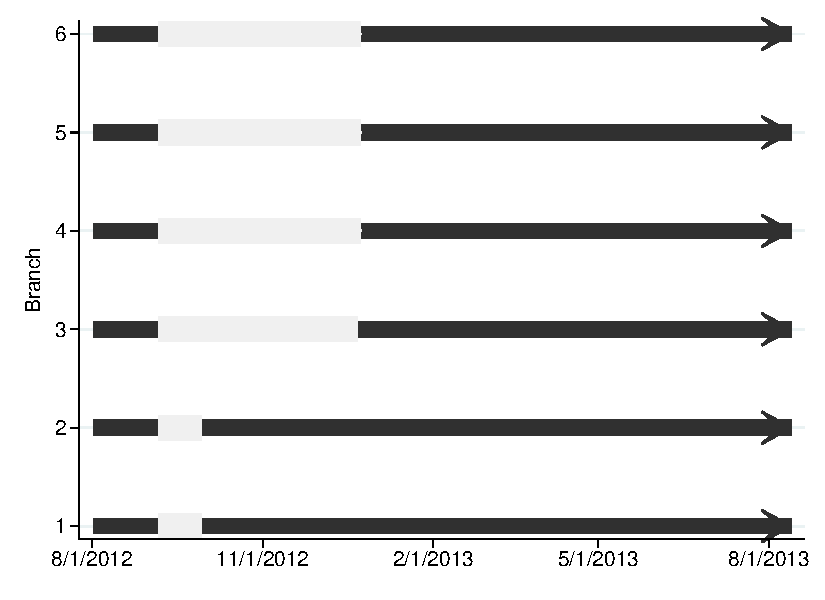
\includegraphics[width=\textwidth]{Figuras/timeline_suc_exp_extended.pdf}
    \end{subfigure}
    \begin{subfigure}{0.40\textwidth}
    \caption{Experiment arms}
       \centering
      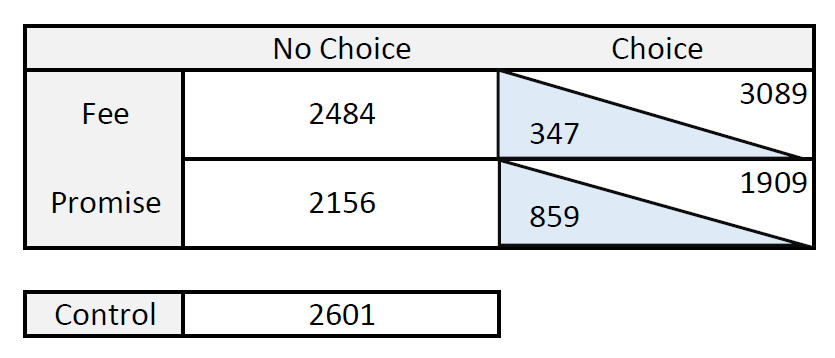
\includegraphics[width=\textwidth]{Figuras/exp_arms.PNG}
    \end{subfigure}
    \end{center}
         \scriptsize Panel (a) displays in black arrows the period covered by our administrative data: from August 6th 2012 (30 days before the experiment began : pre-experiment period) to August 13th 2013. The gray lines correspond to the dates of implementation of the experiment. We finished the experiment earlier in branches 1 and 2 because we realized that we would have enough sample size with the remaining branches and wanted to save on operational costs. Panel (b) shows our 5 treatment arms: control (status quo contract), no fee-forcing, promise-forcing, choice among status quo and fee-commitment, and choice among status quo promise-commitment. Within each arm it displays the number of observations. For the choice groups it splits the sample size into those who chose the commitment contract (shaded blue triangle) and those that did not (un-shaded triangle).
%\textit{Do file: }  \texttt{timeline\_suc\_exp.do}
\end{figure}



\begin{figure}[H]
     \caption{Explanatory Material: Promise-Choice Days}
    \label{ExplanatoryMaterial}
    \begin{center}
    \begin{subfigure}{0.75\textwidth}
        \centering
        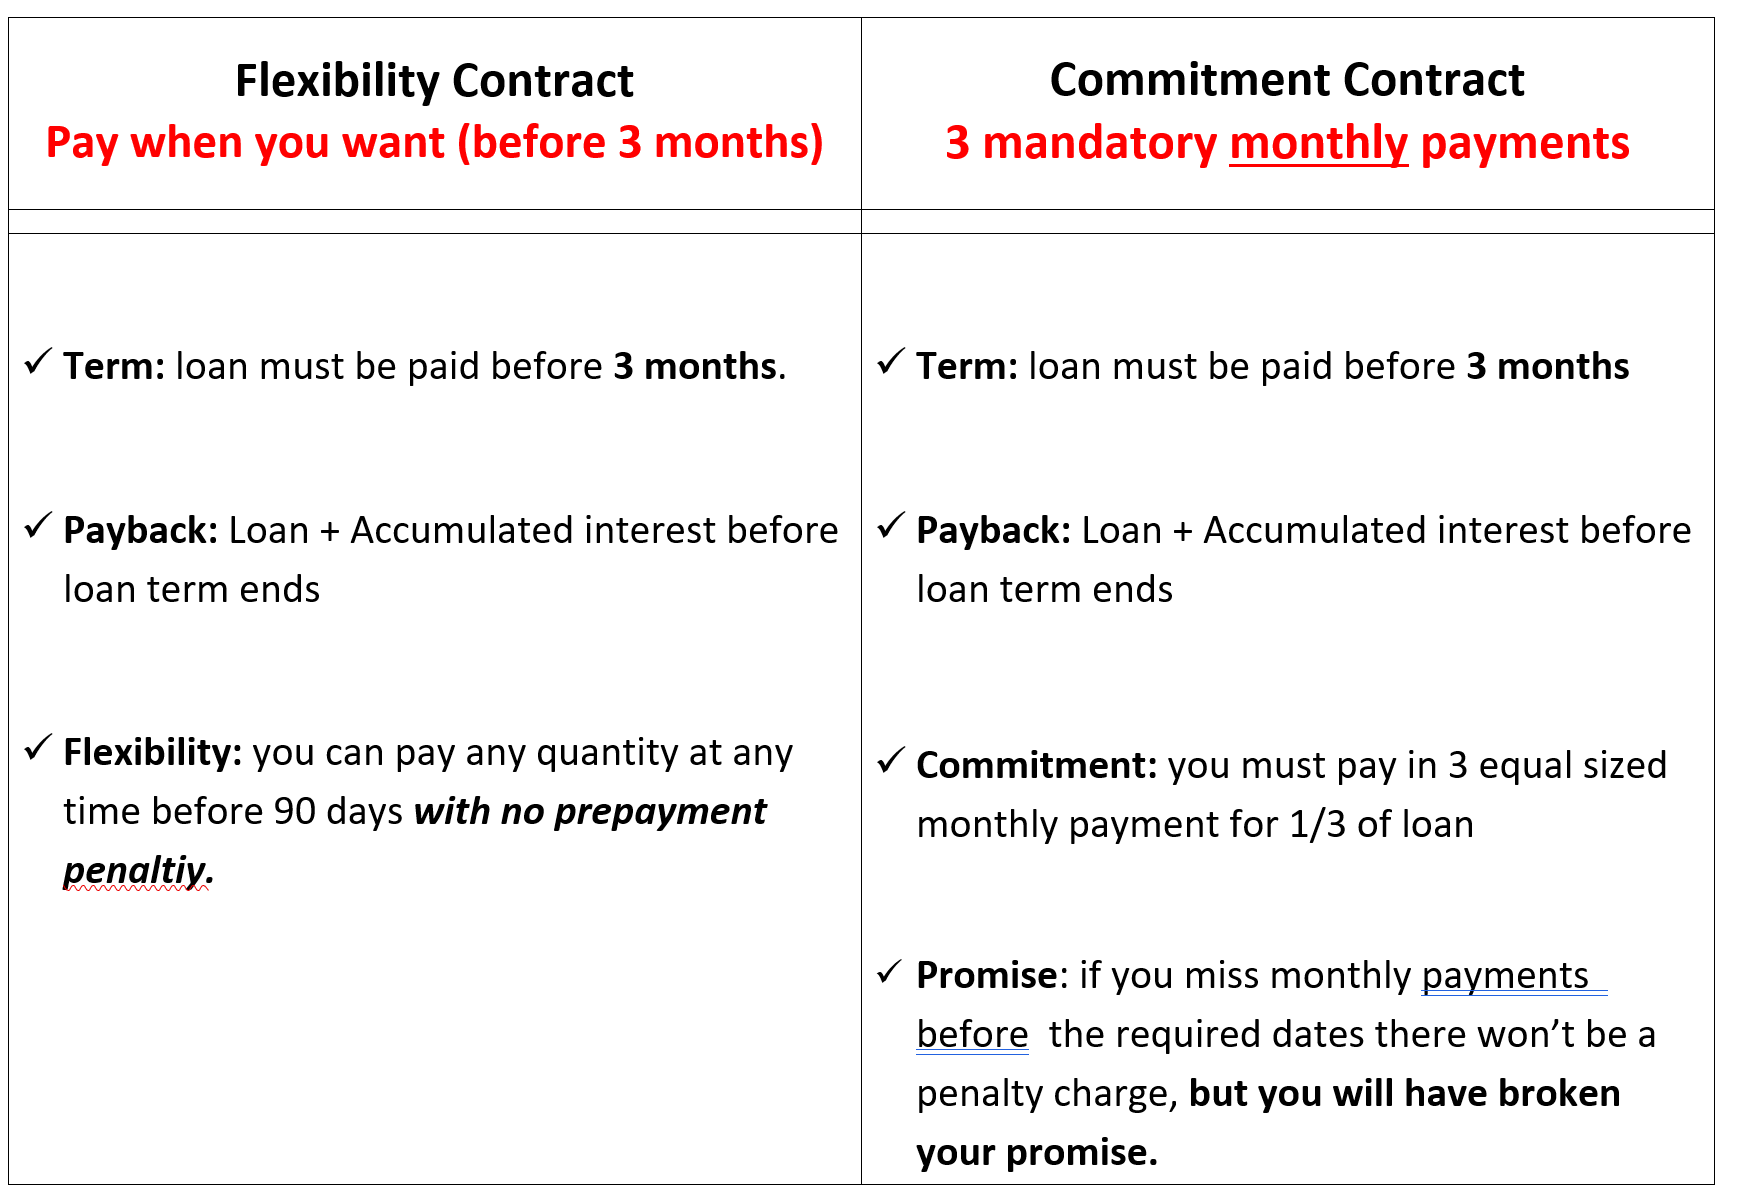
\includegraphics[width=\textwidth]{Figuras/MicaChoiceDonde.png}
    \end{subfigure}
    \end{center}
    \scriptsize
        This is a (translated) sample information slide shown to clients in choice-promise days. The real ones were twice the size of this figure and were laminated. Different ones were shown for each treatment arm.
\end{figure}




\vspace{.2in}
\begin{figure}[H]
     \caption{Financial cost}
    \label{fc_hist}
    \begin{center}
    \begin{subfigure}{.45\textwidth}
      \caption{In pesos MXN}
        \centering
        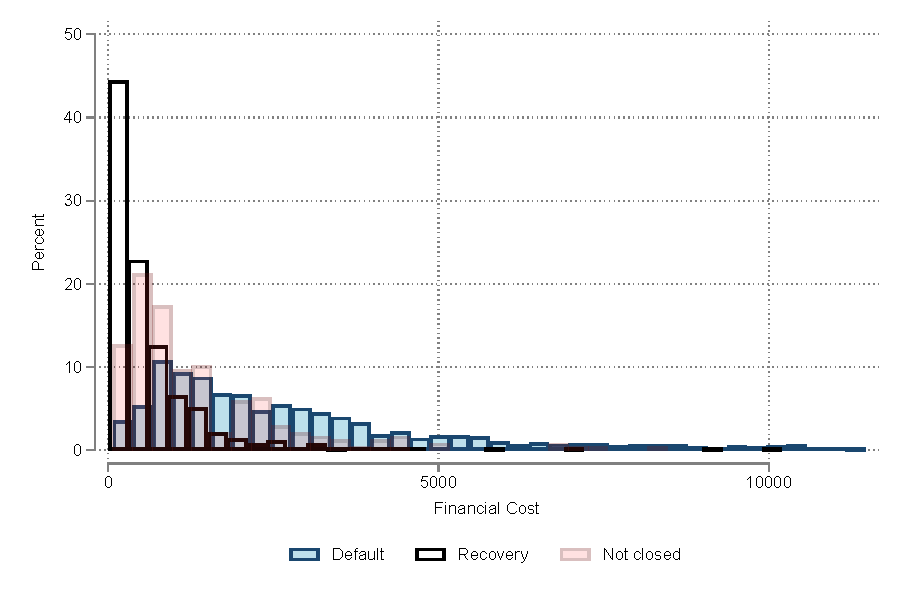
\includegraphics[width=\textwidth]{Figuras/hist_fc.pdf}
    \end{subfigure}
    \begin{subfigure}{0.45\textwidth}
    \caption{As a fraction of the loan}
       \centering
      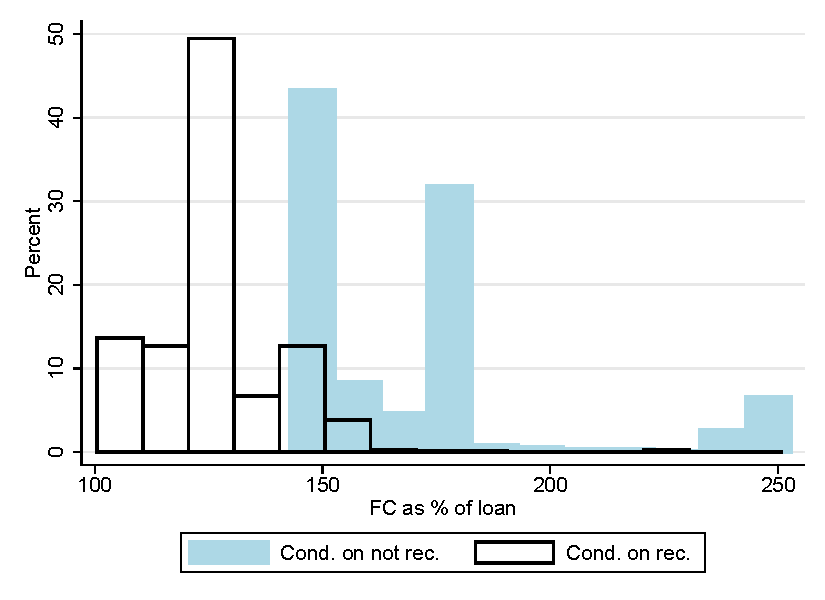
\includegraphics[width=\textwidth]{Figuras/hist_fc_perc_loan.pdf}
    \end{subfigure}
     \begin{subfigure}{0.45\textwidth}
    \caption{Effective cost-loan ratio}
       \centering
      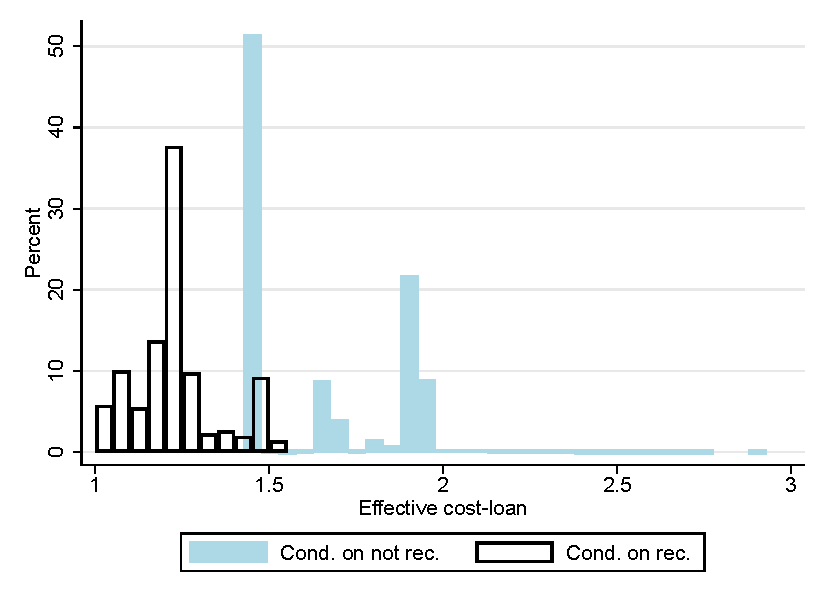
\includegraphics[width=\textwidth]{Figuras/hist_eff.pdf}
    \end{subfigure}
    \end{center}
         \scriptsize
         Panel (a) presents a histogram of financial cost for the control group. Financial cost is defined as the sum of payments made by a client towards recovering her pawn + the cost of the pawned piece when she ends up losing it. In the paper we use different costs of losing the pawn: its value in gold, or the self reported subjective (e.g. jewelry may have sentimental value). This Figure uses the gold value. We plot separately the financial cost for those who lose the pawn (blue) and those that recover it (transparent).  Panel (b) is analogous but we normalized the financial cost, dividing it by the loan size.  %Given that the loan lasts close to 90 days, bringing payments to present value makes little difference. 
      %\footnotesize{ } \textit{Do file: }  \texttt{hist\_eff.do}
\end{figure}






\begin{figure}[H]
    \caption{The effect of the fee-forcing treatment}
    \label{fc_pro2}
    \begin{center}
    \begin{subfigure}{0.42\textwidth}
        \caption{Financial cost (MXN)}
        \centering
        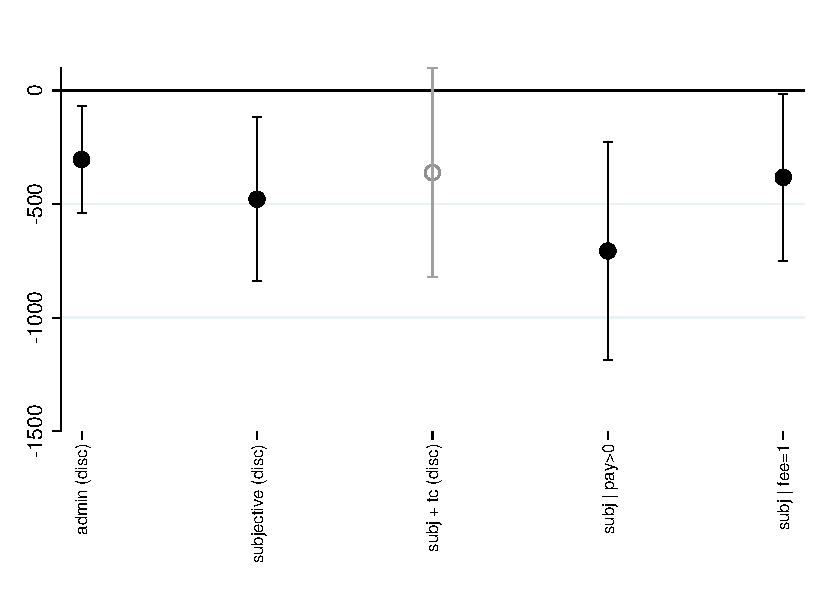
\includegraphics[width=\textwidth]{Figuras/fc_te_pro_2.pdf}
    \end{subfigure}
        \begin{subfigure}{0.42\textwidth}
        \caption{Financial cost (quantile reg)}
        \centering
        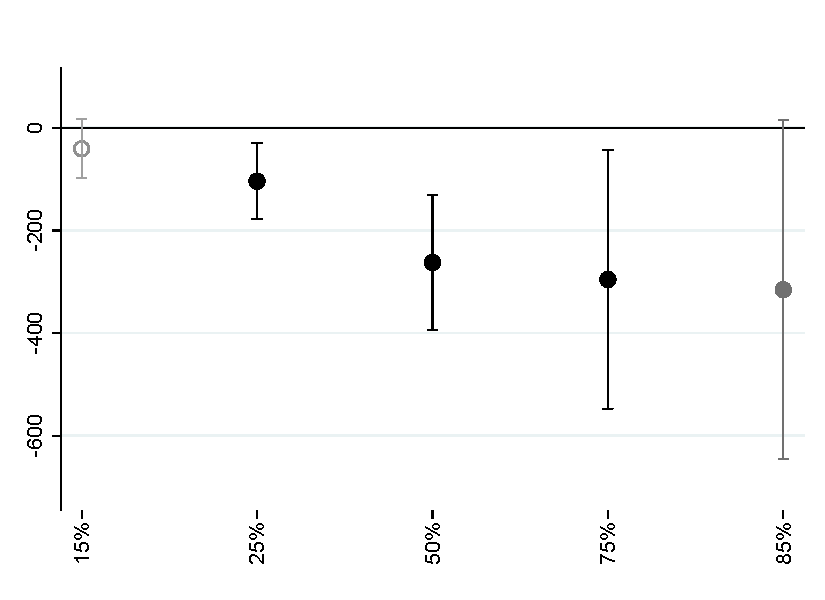
\includegraphics[width=\textwidth]{Figuras/fc_quantile_pro_2.pdf}
    \end{subfigure}
    
        \bigskip
    
    \begin{subfigure}{0.42\textwidth}
        \caption{Financial cost (HTE)}
        \centering
        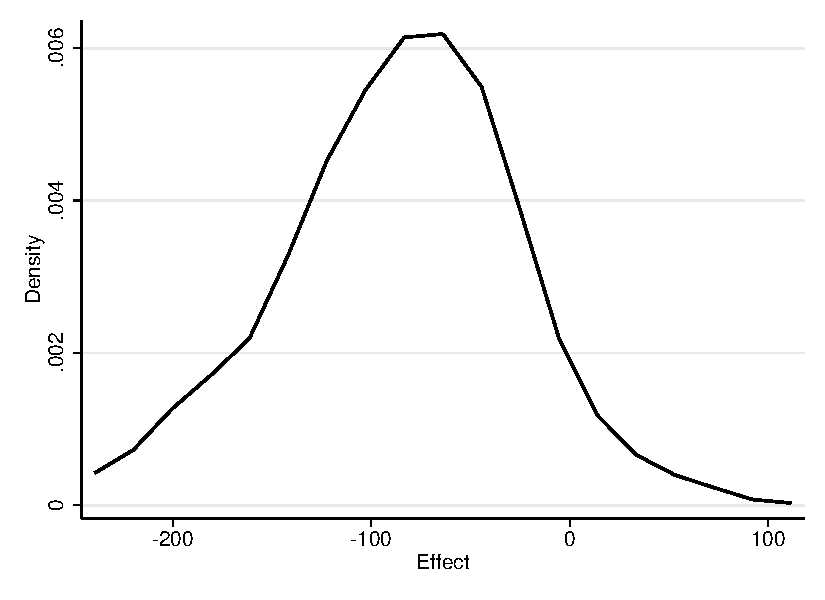
\includegraphics[width=\textwidth]{Figuras/he_dist_fc_admin_disc_pro_2.pdf}
    \end{subfigure}
    ~
    ~
    \bigskip
    \begin{subfigure}{0.42\textwidth}
        \caption{Lost pawn}
        \centering
        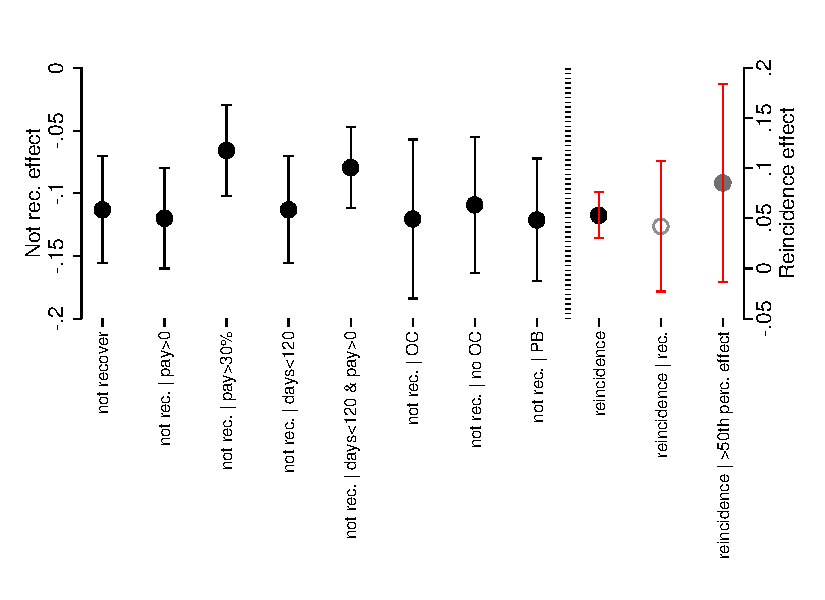
\includegraphics[width=\textwidth]{Figuras/def_te_pro_2.pdf}
    \end{subfigure}
    \begin{subfigure}{0.42\textwidth}
    \caption{Losing Pawn}
        \centering
        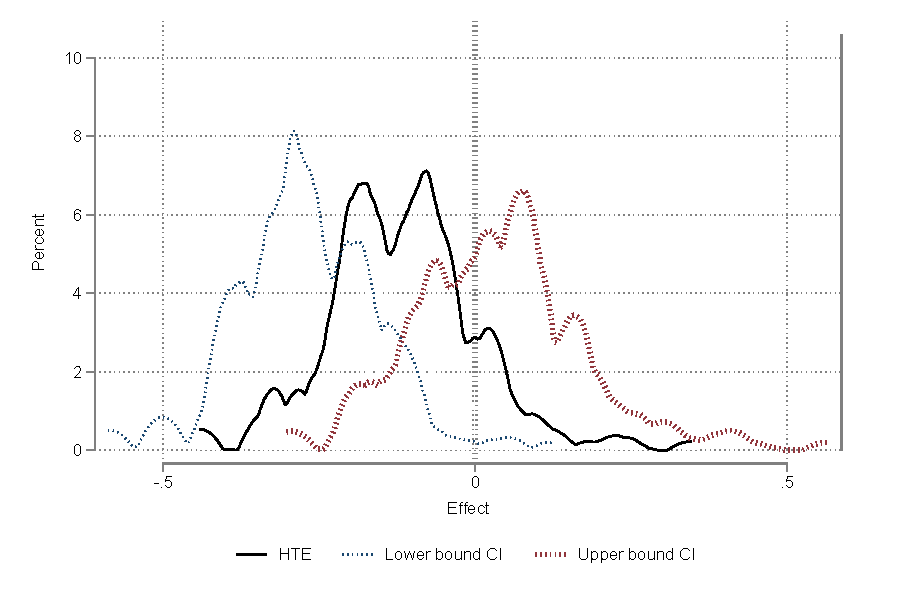
\includegraphics[width=\textwidth]{Figuras/he_dist_def_c_pro_2.pdf}
    \end{subfigure}

    \end{center}
        \scriptsize 
        
      %\textit{Do file: }  \texttt{fc\_te.do, def\_te.do, fc\_quantilereg.do}
\end{figure}

\scriptsize {
\noindent This figure shows the estimated treatment effect of ``forcing'' the frequent payment commitment contract using fees, compared to the status-quo (control). In Panel (a) each dot represents the estimated treatment effect for a different definition of financing cost, or for a different sub-population, and its 95\% confidence interval. From left to right, the first effect corresponds to using the gold value of the pawned piece in the definition of financial cost and discounting the payments to present value using a 7\% monthly rate - to the left we have a decomposition of the financial cost in its four components from left to right (1) Discounted payments to capital, (2) Payed fees, (3) Payed interest, (4) Cost of losing pawn; the second uses the subjective value of the pawn; the third is analogous to the second but adds transaction cost (transport+1 day's wage) per visit; the fourth conditions on the population that paid any positive amount towards recovery of their pawn; the fifth conditions on the sub-population of the treatment group that paid a fee and compares these to all the control group. Panel (b) plots the effects on different quantiles of the distribution of financial cost (using the first definition): 15th, 25th, 50th, 75th, 85th percentile. Panel (c) plots the distribution of the heterogeneous treatment effects on financial cost, estimated using \cite{atheygrf}. Panel (d) Measures the effect of treatment on the likelihood of losing their pawn. The first coefficient compares all the treatment group vs all the control using 230 days after pawning to define the dependent variable; the second defines it using 120 days. The third coefficient from the left conditions on the population that paid any positive amount towards recovery of their pawn (which in theory may be endogenous but empirically we showed not to be affected by treatment). Finally, Panel (e) shows the distribution of heterogeneous treatment effects of the probability of losing the pawn. % the effect on ``repeat purchase''. That is likelihood of doing an additional pawn (in treatment vs control) after having been subjected to treatment for at least 75 days. The second coefficient estimates the regression conditional on recovering the pawn {in both treatment and control}, and the rightmost coefficient compares those above the median treatment effect in financial cost savings, {versus all the control group.}
}


\begin{figure}[H]
    \caption{The effect of the fee-forcing treatment}
    \label{fc_pro2}
    \begin{center}
    \begin{subfigure}{0.42\textwidth}
        \caption{Effective cost/loan ratio}
        \centering
        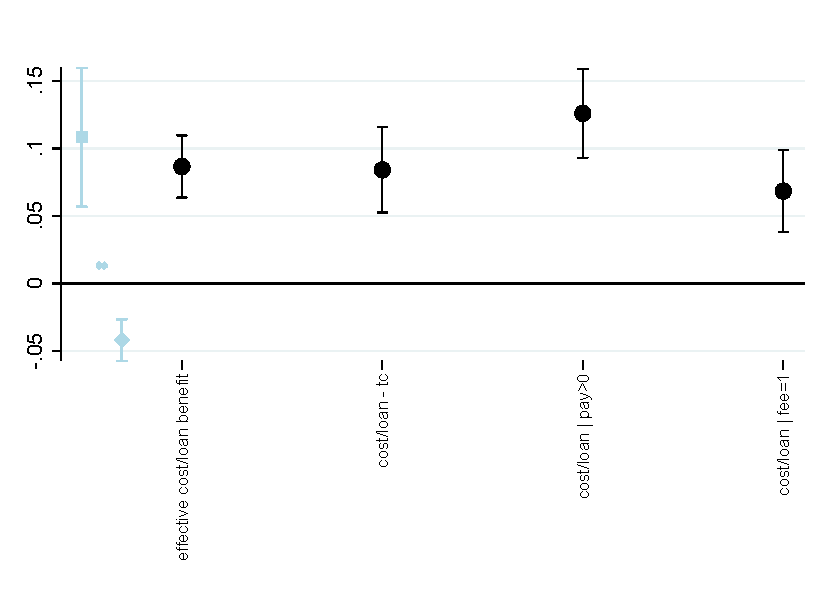
\includegraphics[width=\textwidth]{Figuras/eff_te_pro_2.pdf}
    \end{subfigure}
        \begin{subfigure}{0.42\textwidth}
        \caption{Financial cost (quantile reg)}
        \centering
        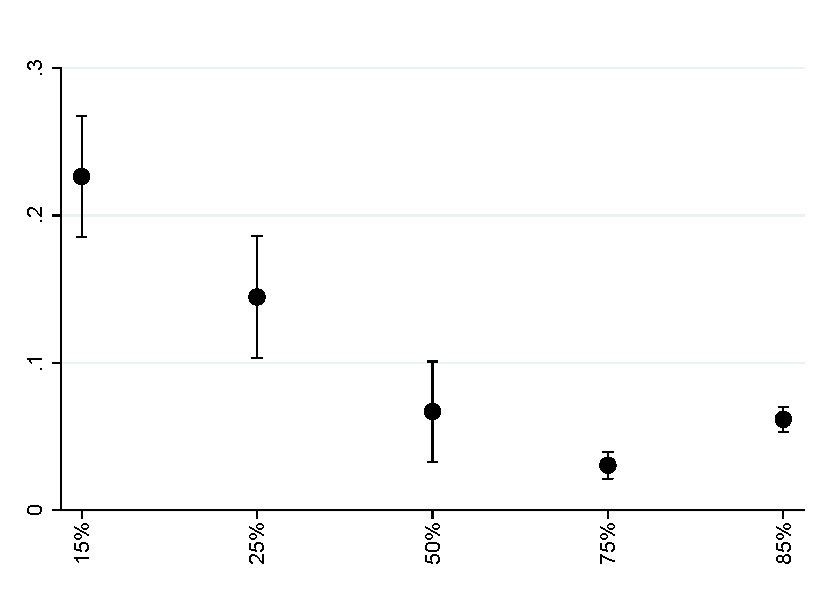
\includegraphics[width=\textwidth]{Figuras/eff_quantile_pro_2.pdf}
    \end{subfigure}
    
        \bigskip
    
     \begin{subfigure}{0.42\textwidth}
         \caption{Financial cost (HTE)}
         \centering
         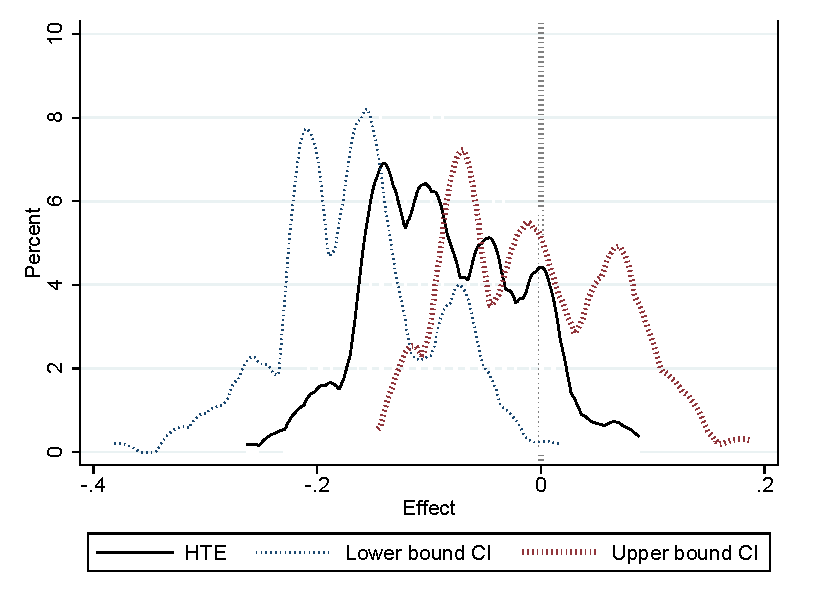
\includegraphics[width=\textwidth]{Figuras/he_dist_eff_cost_loan_pro_2.pdf}
     \end{subfigure}
    ~
    ~
    \bigskip
    \begin{subfigure}{0.42\textwidth}
        \caption{Lost pawn}
        \centering
        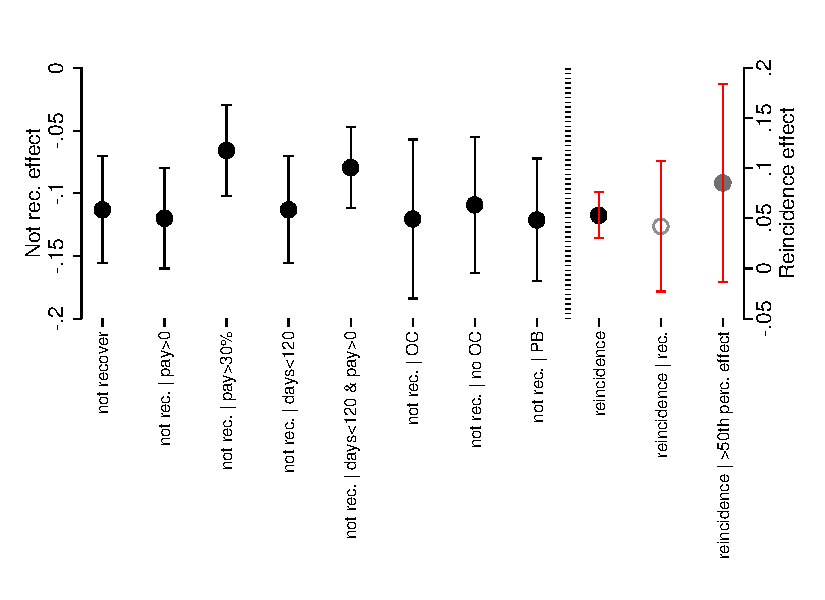
\includegraphics[width=\textwidth]{Figuras/def_te_pro_2.pdf}
    \end{subfigure}
    \begin{subfigure}{0.42\textwidth}
    \caption{Losing Pawn}
        \centering
        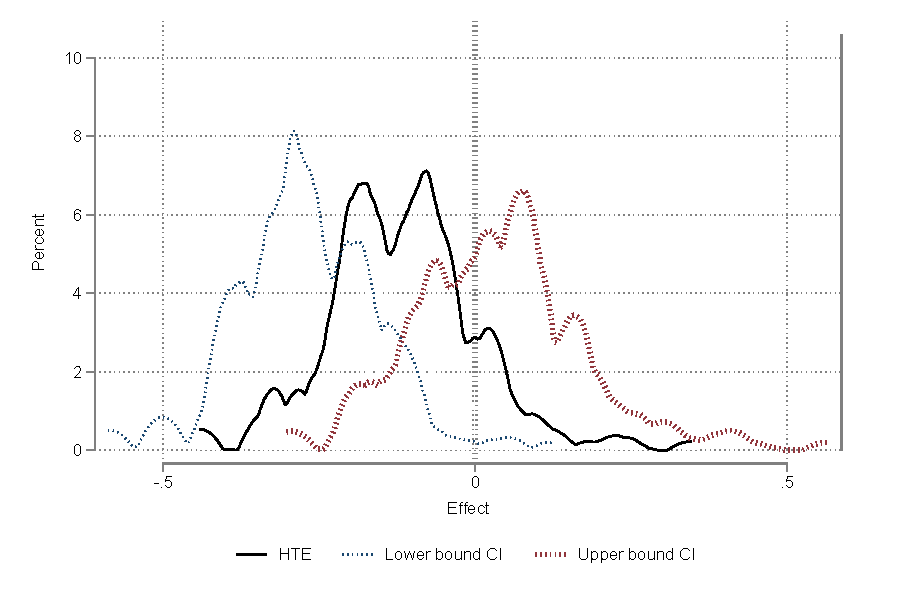
\includegraphics[width=\textwidth]{Figuras/he_dist_def_c_pro_2.pdf}
    \end{subfigure}

    \end{center}
        \scriptsize 
        
      %\textit{Do file: }  \texttt{eff\_te.do, def\_te.do, eff\_quantilereg.do}
\end{figure}

\vspace{3ex}

\vspace{.3in}
\begin{figure}[H]
        \caption{Effects on repeat purchasing}
    \label{reincidence}
    \begin{center}
        \centering
        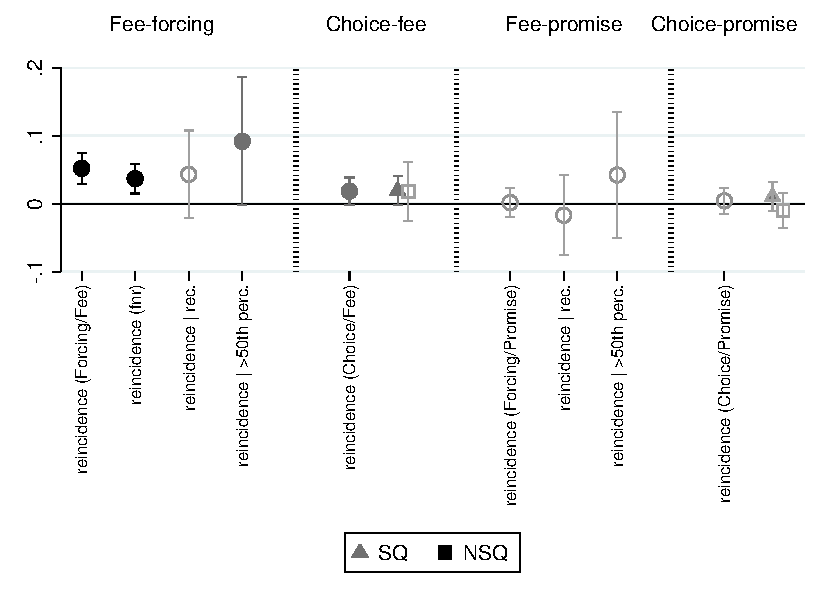
\includegraphics[width=0.6\textwidth]{re_te.pdf}
    \end{center}
     \scriptsize This figure shows the estimated effects on repeat purchasing of the four treatment arms (fee-forcing, choice-fee, fee-promise, choice-promise) compared to the status-quo control group. It shows robustness of the effects by focusing on different sub-populations. The leftmost coefficient compares all the fee-forcing group against all status quo group. The second coefficient conditions on the first pawn not being recovered when the second was pawned. The third coefficient conditions on clients who pawned again after having recovered the pawn in the experiment. The fourth coefficient uses all clients (in both the fee-forcing and the status-quo arms) who had an estimated heterogeneous treatment effect above the median. Conditioning on this set keeps the sample balanced across arms and therefore still allows for a causal interpretation. For the choice arm we present three coefficients: coefficients represented by a circle compare all those offered choice to all those in the status quo arm, thus estimating a causal effect. Coefficients in triangles and squares represent those that self-select into the fee or promise arms and compare this subset against the whole status quo arm. They therefore contain a selection effect together with the treatment effect and cannot be interpreted causally.
      %\footnotesize{ \textit{Do file: }  \texttt{re\_te.do}
\end{figure}




\begin{figure}[H]
    \caption{The effect of choice between fee-commitment and status quo}
    \label{fc_pro4}
    \begin{center}
    \begin{subfigure}{0.45\textwidth}
        \caption{Financial cost}
        \centering
        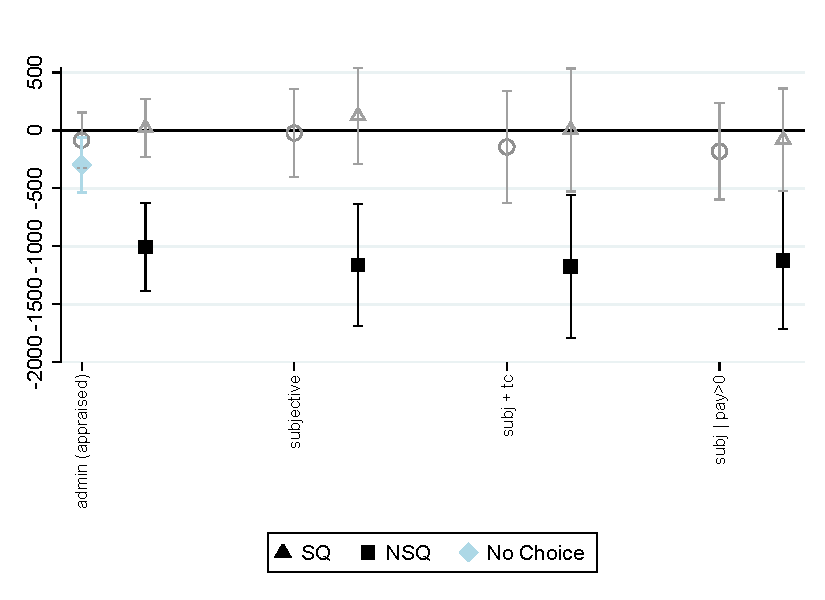
\includegraphics[width=\textwidth]{Figuras/fc_te_pro_4.pdf}
    \end{subfigure}
        \begin{subfigure}{0.45\textwidth}
        \caption{Financial Cost (quantile reg)}
        \centering
        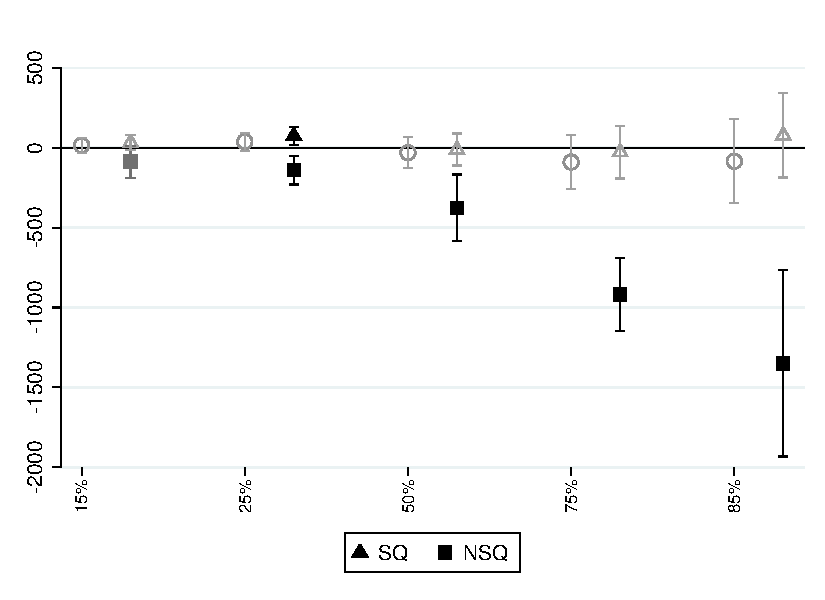
\includegraphics[width=\textwidth]{Figuras/fc_quantile_pro_4.pdf}
    \end{subfigure}
    \begin{subfigure}{0.5\textwidth}
    
        \bigskip
        \bigskip
    
        \caption{Lost Pawn}
        \centering
        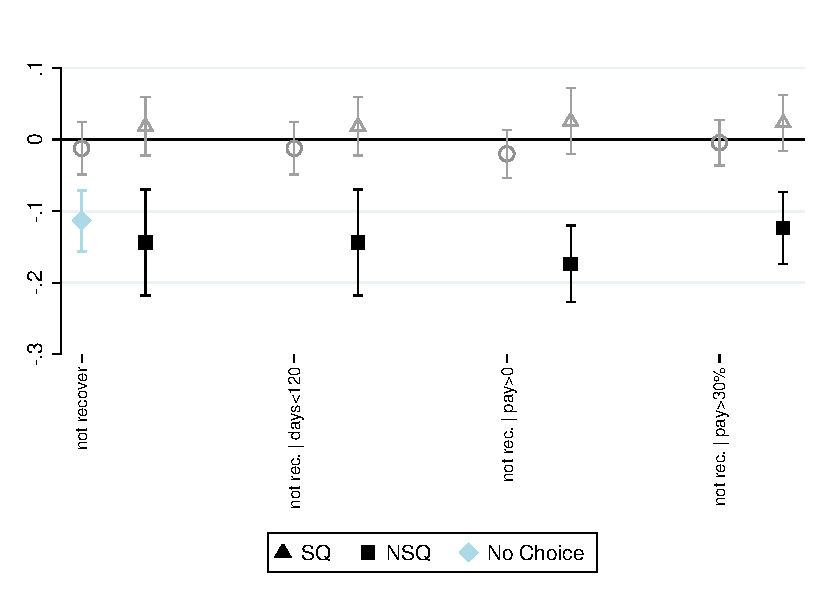
\includegraphics[width=\textwidth]{Figuras/def_te_pro_4.pdf}
    \end{subfigure}
    \end{center}
        \scriptsize
        This figure is analogous to Figure \ref{fc_pro2}. It measures the effect of being given \textit{choice} between the frequent payment commitment contract with fees and the status-quo contract, versus being \textit{``forced''} into the status-quo contract (control). Again it focuses our two main outcomes: financial cost and an indicator for losing the pawn. Circles present the treatment effects. The figures also presents differences in these two outcomes for those who chose the frequent payment commitment contract versus the whole control group (squares-NSQ), and also for those who chose the status quo contract versus the whole control group (triangles-SQ). Note that these two comparisons are not pure causal effects since people who chose the frequent payment commitment contract are different from those that do not. That is: the squares and triangles combine selection and treatment effects. Finally, for comparison purposes, the blue diamond displays the effects of forcing them into the frequent payment commitment contract and are just transcribed from Figure \ref{fc_pro2} above. 
      %\textit{Do file: }  \texttt{fc\_te\_choice\_dec.do, def\_te\_choice\_dec.do, fc\_quantilereg\_choice\_dec.do}
\end{figure}





\begin{figure}[H]
        \caption{Distribution of Overconfidence}
    \label{oc_hist}
    \begin{center}
        \centering
        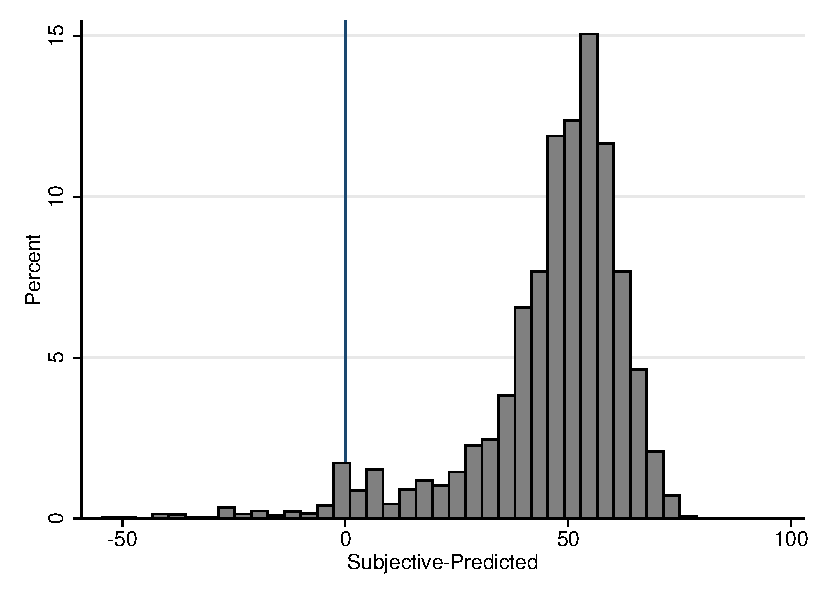
\includegraphics[width=0.55\textwidth]{Figuras/oc_hist.pdf}
    \end{center}
    \scriptsize
     In the baseline survey at the branch, before the client knew the contract or had the pawn appraised, they were asked from 0 to 100, how likely it was that they would be able to recover their pawn if pawned. We generate a variable we call overconfidence (OC) defined as the reported subjective probability of recovery minus the predicted probability ($P^s_i-\widehat{P_i(X_i)}$). We predict $\widehat{P_i(X_i)}$ using LASSO as explained in the text. This figure uses all observations for which we have data on $P^s_i$ and $X_i$ from the baseline survey.
     %\textit{Do file: }  \texttt{oc.do}
     
\end{figure}






\begin{figure}[H]
    \caption{Choice of contracts and treatment effects}
    \label{choose_wrong}
    \begin{center}
        \begin{subfigure}{0.45\textwidth}
        \caption{Chose wrong}
        \centering
        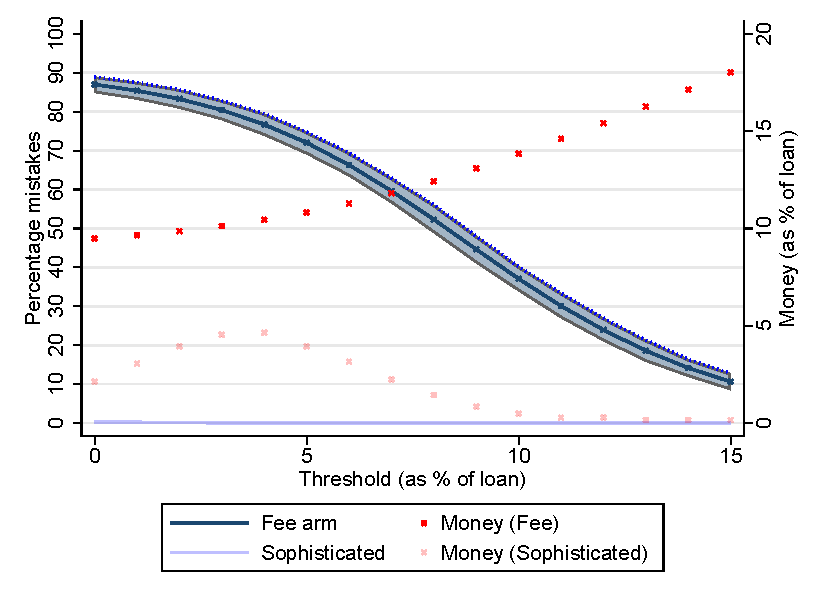
\includegraphics[width=\textwidth]{Figuras/line_cw_eff_te_cf.pdf}
        
    \end{subfigure}
        \begin{subfigure}{0.45\textwidth}
        \caption{By overconfidence/naivete}
        \centering
        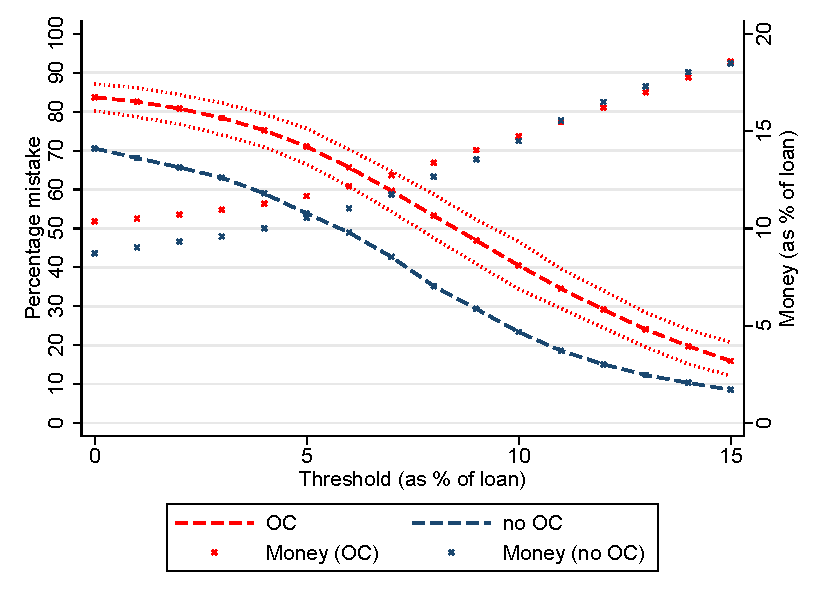
\includegraphics[width=\textwidth]{Figuras/line_cw_eff_te_cf_OC_fee.pdf}

    \bigskip
        
    \end{subfigure}
        \begin{subfigure}{0.45\textwidth}
        \caption{\% better when forced to fee-commitment}
        \centering
        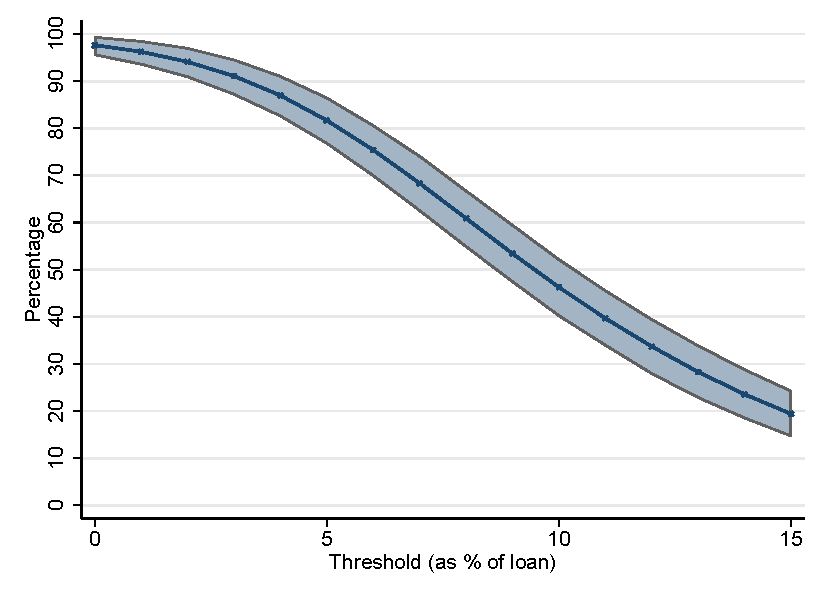
\includegraphics[width=\textwidth]{Figuras/line_better_forceall_eff_te_cf.pdf}
        
    \end{subfigure}
        \begin{subfigure}{0.45\textwidth}
        \caption{\footnotesize{Effect of losing pawn vs predicted take-up}}
        \centering
        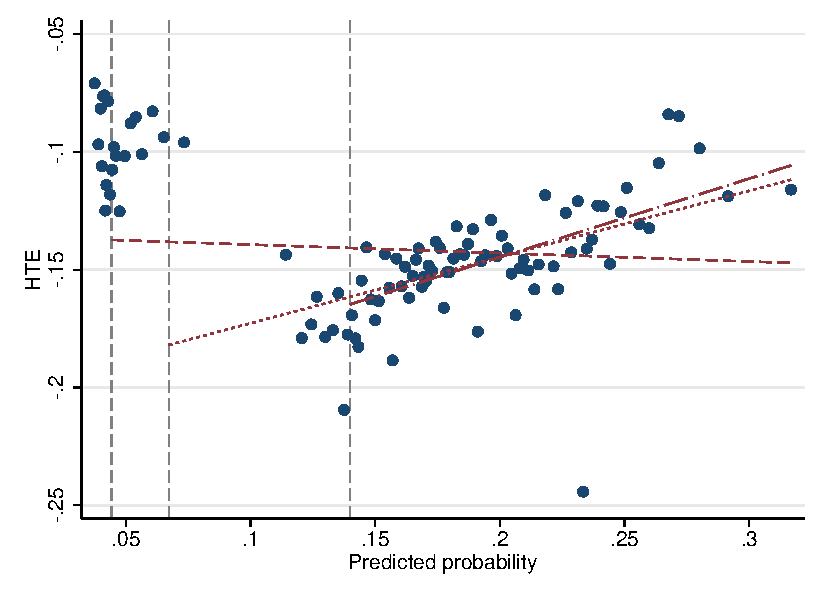
\includegraphics[width=\textwidth]{Figuras/takeuppr_def.pdf}
    \end{subfigure}
    
    \end{center}
        \scriptsize
        In Panel (a) we estimate what the treatment effect of the commitment contract \textit{would have been} for all subjects in the choice arm if they had been forced into the fee-commitment contract. To do this we proceed in two steps. First, we estimate treatment effects in the forcing arm by comparing the fee-forcing arm against the status quo arm. We let these effects be heterogeneous as a function of our $x$'s using \cite{atheygrf}'s methodology of causal forests. Second, we extrapolate these treatment effects based on the choice arm using the same $x$'s. Once we have personalized counterfactual treatment effects in the choice arm we calculate what fraction of subjects in the choice arm incurred in financial costs that are  $> z$\% than if they had chosen the opposite contract of what they actually chose, were $z$\% is defined as a fraction of the loan. $z$\% is a level of tolerance we can vary and we plot it in the X-axis. The left Y-axis measures the fraction of subjects that would have been better by a margin of $z$\% if they changed their choice, and the right Y-axis measures the amount of money ``left on the table''. We use bootstrap to tighten the confidence intervals (CIs). \cite{atheygrf}'s heterogeneous treatment effect using GRF is asymptotically normal. We compute the HTE ($\mu$) together with standard errors ($\sigma$) . For every pledge, we draw a random effect from a normal distribution with parameters ($\mu$,$\sigma^2$), and compute via bootstrap the percentage that choose wrong, along normal-approximation CIs (results are robust if we use instead percentile CIs or bias-corrected CIs) . This allows us to estimate a distribution for the upper and lower bound CIs, which we then use to obtain a 95\% CI. Panel (b) is analogous to Panel (a) except that it does the exercise separately for clients we classified as overconfident ($OC_i:=\mathbbm{1}(P^s_i-\widehat{P_i(X_i)}>0))$ and those we classified as not overconfident. Panel (c) simulates what percentage would be better by at least $z$ if we forced everybody of those in the fee-choice arm into the fee-commitment contract. Panel (d) asks whether it is the case that people with larger causal benefits from the fee-forcing contract would be more likely to select that contract. To do this we proceed in two steps as well. First we estimate a flexible model of take-up of the fee commitment contract \textit{in the choice arm} using random forests, and from this model obtain a probability $P(x_i)$ of choosing the fee-forcing contract for a client with characteristics $x_i$. We extrapolate this model to clients in the fee-forcing arm to estimate what would they have chosen if we had given them choice. Figure (d) plots $\widehat{P(x_i)}$ in the X-axis using a binscatter that splits the X-axis in 100 percentile bins. The Y-axis plots the heterogeneous treatment effects of the fee forcing contract on the probability of losing the pawns (more negative means then more likely to recover it), averaged for the respective x-axis bin. Positive assortative selection would mean a negative relationship: those who benefit more by treatment and lose the pawn less are \emph{less} likely to choose it.  Using all bins we estimate a slope of zero in the relationship. Using the 80 right most points, we estimate a \textit{positive} relationship.
        %\textit{Do file: }  \texttt{effect\_contr\_takeup.do, choose\_wrong\_quant\_wrong.do, choose\_wrong\_quant\_wrong\_decomposition.do}
\end{figure}






\begin{figure}[H]
    \caption{The effect of promises}
    \label{fc_pro5}
    \begin{center}
    

        \begin{subfigure}{0.45\textwidth}
        \caption{Financial cost -- Choice}
        \centering
        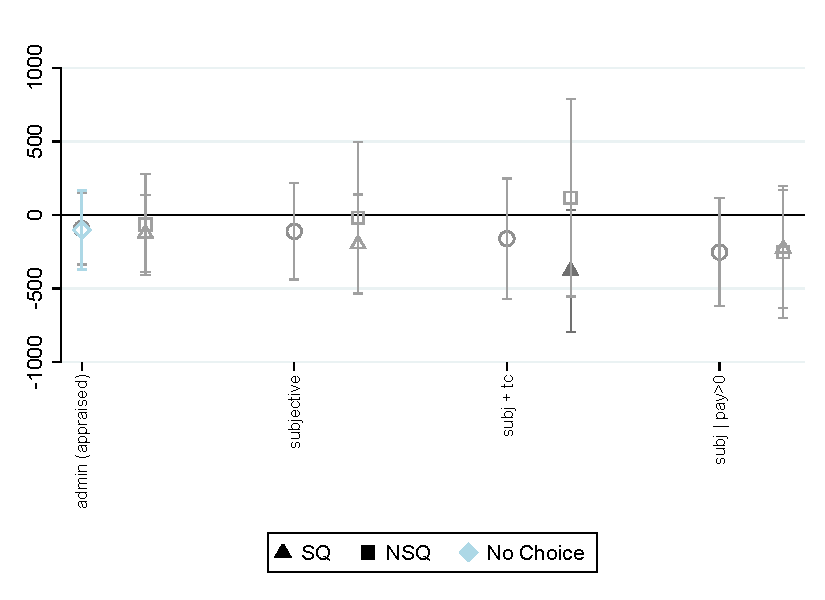
\includegraphics[width=\textwidth]{Figuras/fc_te_pro_5.pdf}
    \end{subfigure}
        %\begin{subfigure}{0.45\textwidth}
        %\caption{Quantile regression}
        %\centering
        %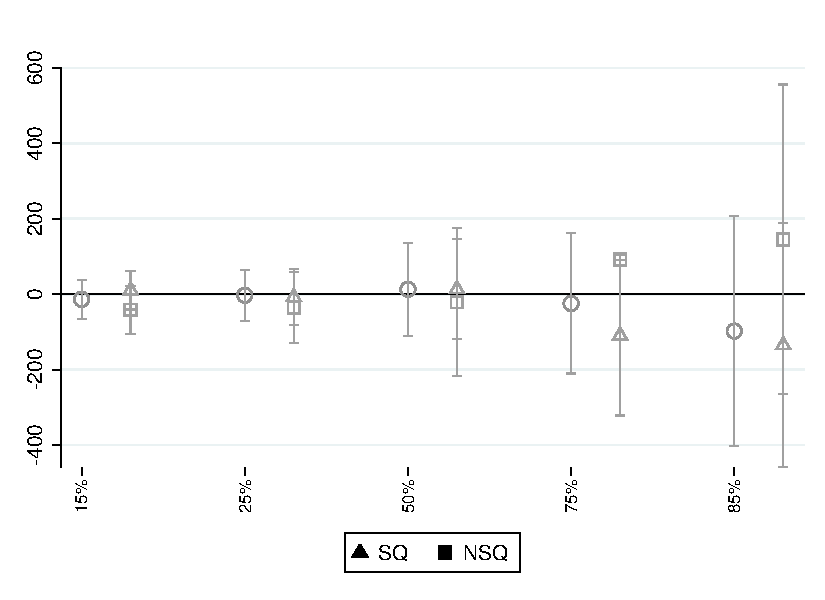
\includegraphics[width=\textwidth]{Figuras/fc_quantile_pro_5.pdf}
    %\end{subfigure}
    \begin{subfigure}{0.45\textwidth}
        \caption{Losing Pawn -- Choice}
        \centering
        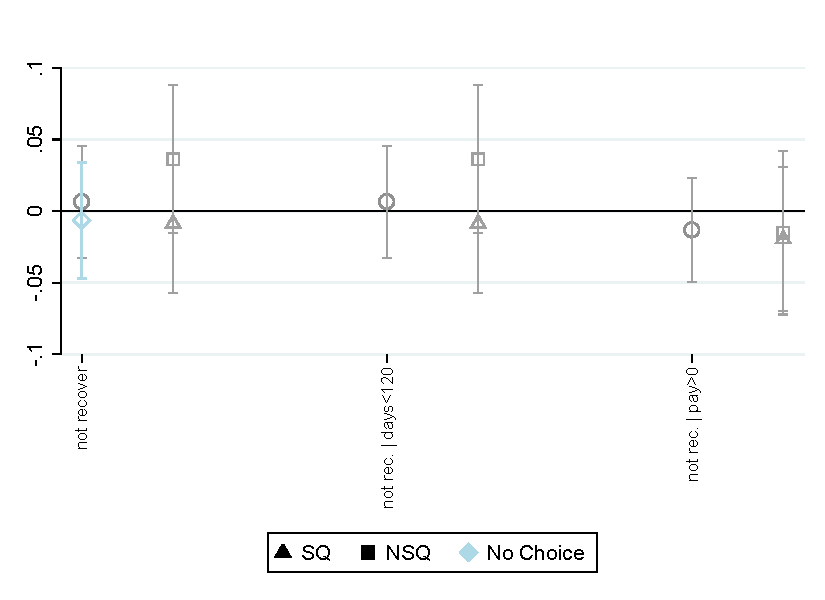
\includegraphics[width=\textwidth]{Figuras/def_te_pro_5.pdf}
    \end{subfigure}
    
    \bigskip
    \bigskip
    
        \begin{subfigure}{0.45\textwidth}
        \caption{Financial cost -- Promise-forcing}
        \centering
        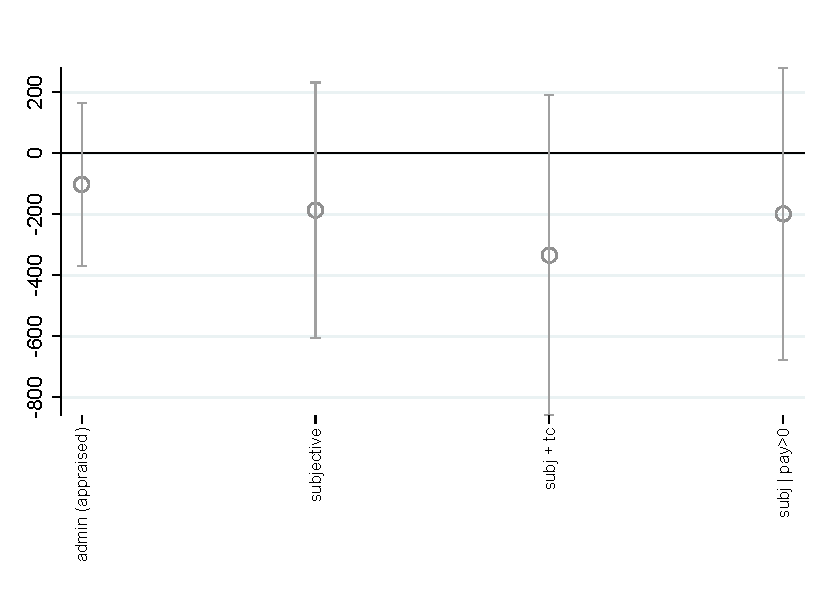
\includegraphics[width=\textwidth]{Figuras/fc_te_pro_3.pdf}
    \end{subfigure}
    \begin{subfigure}{0.45\textwidth}
        \caption{Losing Pawn -- Promise-forcing}
        \centering
        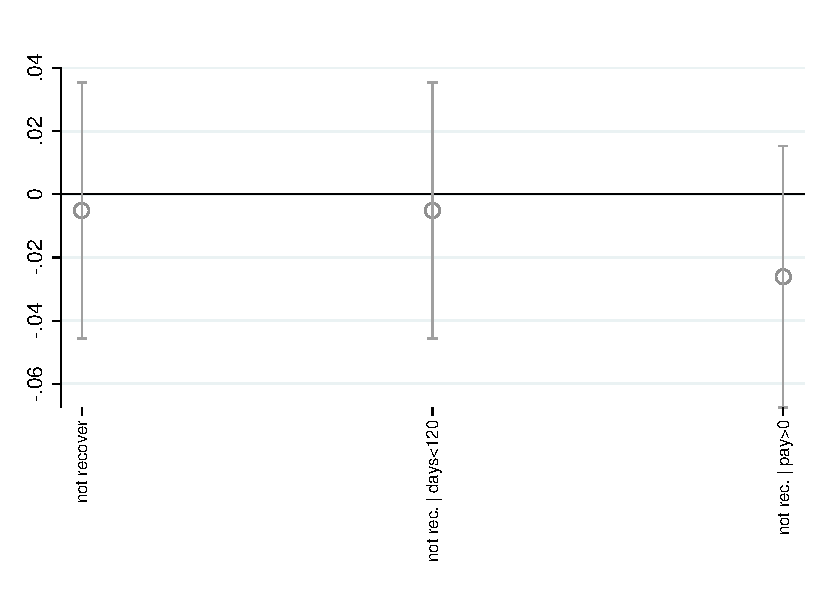
\includegraphics[width=\textwidth]{Figuras/def_te_pro_3.pdf}
    \end{subfigure}
    

    
    
    \end{center}
    \scriptsize
    Panels (a) and (b) in this figure show the estimated treatment effects of ``forcing'' the frequent payment commitment contract using promises, compared to the status-quo (control) for financial cost (Panel a), and for an indicator of losing the pawn (Panel b). Panels (c) and (d) are analogous but focus on the effect of giving choice between frequent payment commitment contract using promises and the status quo contract. In Panel (a) each dot represents the estimated treatment effect for a different definition of financing cost, or for a different sub-population, and its 95\% confidence interval. From left to right, the first effect corresponds to using the gold value of the pawned piece in the definition of financial cost and discounting the payments to present value using a 7\% monthly rate; the second uses the subjective value of the pawn; the third is analogous to the second but adds transaction cost (transport+1 day's wage) per visit; and the fourth conditions on the population that paid any positive amount towards recovery of their pawn. Panel (b) plots the effect of not recovering the pawn: the leftmost coefficients compares all those assigned to the promise-forcing arm vs all those in the status quo contract, where the dependent variable=1 if the client has not recovered the pawn 230 days after pawning. The next coefficient defines the dependent variable=1 if the client has not recovered the pawn 120 days after pawning. The third coefficient conditions on paying a positive amount, and the fourth conditions on paying at least 30\% of the loan.   Panels (b) and (c) measure the effect of being given \textit{choice} between the frequent payment commitment contract with promise and the status-quo contract, versus being \textit{``forced''} into the status-quo contract (control). Again it focuses our two main outcomes: financial cost and an indicator for losing the pawn. Circles present the treatment effects. The figures also presents differences in these two outcomes for those who chose the frequent payment commitment contract versus the whole control group (squares-NSQ), and also for those who chose the status quo contract versus the whole control group (triangles-SQ). That is: the squares and triangles combine selection and treatment effects.
      %\footnotesize{ } \textit{Do file: }  \texttt{fc\_te\_choice\_dec.do, def\_te\_choice\_dec.do, fc\_te.do, def\_te.do }
\end{figure}




%\begin{figure}[H]
%    \caption{The effect of the promise-forcing treatment}
%    \label{fc_pro3}
%    \begin{center}
%        \begin{subfigure}{0.45\textwidth}
%        \caption{Quantile regression}
%        \centering
%        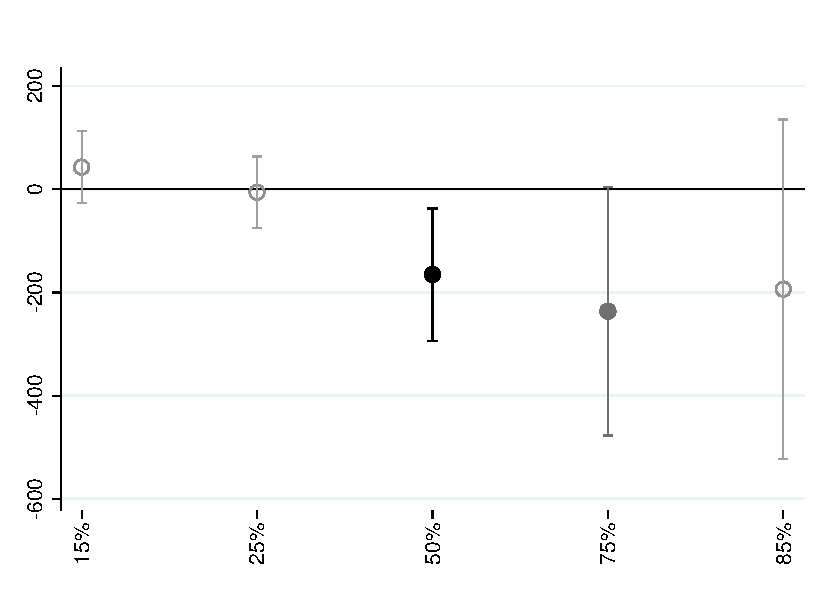
\includegraphics[width=\textwidth]{Figuras/fc_quantile_pro_3.pdf}
%    \end{subfigure}
%    
%    \end{center}
%             \footnotesize \textit{Notes: } 
%      \footnotesize{ } \textit{Do file: }  \texttt{fc\_te.do, def\_te.do, fc\_quantilereg.do}
%\end{figure}



\newpage


%%%%%%%%%%%%%%%%%%%%%%%%%%%%%%%%%%%%%%%%%%%%%%%

% APPENDIX 
\setcounter{table}{0}
\setcounter{figure}{0}
\setcounter{section}{0}
\pagenumbering{gobble}


\begin{center}
	\LARGE The limits of self-commitment and private paternalism \\[0.5em]
	\Large{Appendix $-$ For Online Publication} \\[1em]
	\large \author{Isaac Meza \and Joyce Sadka \and Enrique Seira}
\end{center}

\appendix
\pagenumbering{arabic}
\renewcommand\thefigure{OA-\arabic{figure}}
\renewcommand\thetable{OA-\arabic{table}}
\renewcommand*{\thepage}{OA - \arabic{page}}
\renewcommand\thesection{Appendix \Alph{section}.}
\renewcommand\thesubsection{\Alph{section}.\arabic{subsection}}

%\renewcommand{\cftparskip}{0em} % NOT NEEDED
\renewcommand\cftsecdotsep{\cftdotsep}
\renewcommand\cftsubsecdotsep{\cftnodots}
\renewcommand{\cftsecnumwidth}{6em}
 \renewcommand{\cftpnumalign}{r}
%\renewcommand{\cftsecleader}{\normalfont\cftdotfill{\cftsecdotsep}}


\renewcommand{\cftsecleader}{\cftdotfill{\cftsecdotsep}\hspace{1.8em}}
%\renewcommand{\cftsecpagefont}{20em}
%\renewcommand{\cftfignumwidth}{6em}
%\renewcommand{\cfttabnumwidth}{3.3em}

%\tableofcontents
\etocdepthtag.toc{mtappendix}
\etocsettagdepth{mtchapter}{none}
\etocsettagdepth{mtappendix}{subsection}

\setstretch{0.9}
%\renewcommand\contentsname{} % the empty name

\begingroup
\let\clearpage\relax
%\vspace{-1.5em} % the removed space. Set as appropriate
\tableofcontents
\endgroup


\newpage



\section{ Further results}
\vspace{.2in}


\subsection{Some materials}

\vspace{.1in}
\begin{figure}[H]
     \caption{Contract Terms Summary, and Promise Slip}
    \label{PaperSlip}
    \begin{center}
    \begin{subfigure}{0.65\textwidth}
    \caption{Receipt for client}
        \centering
        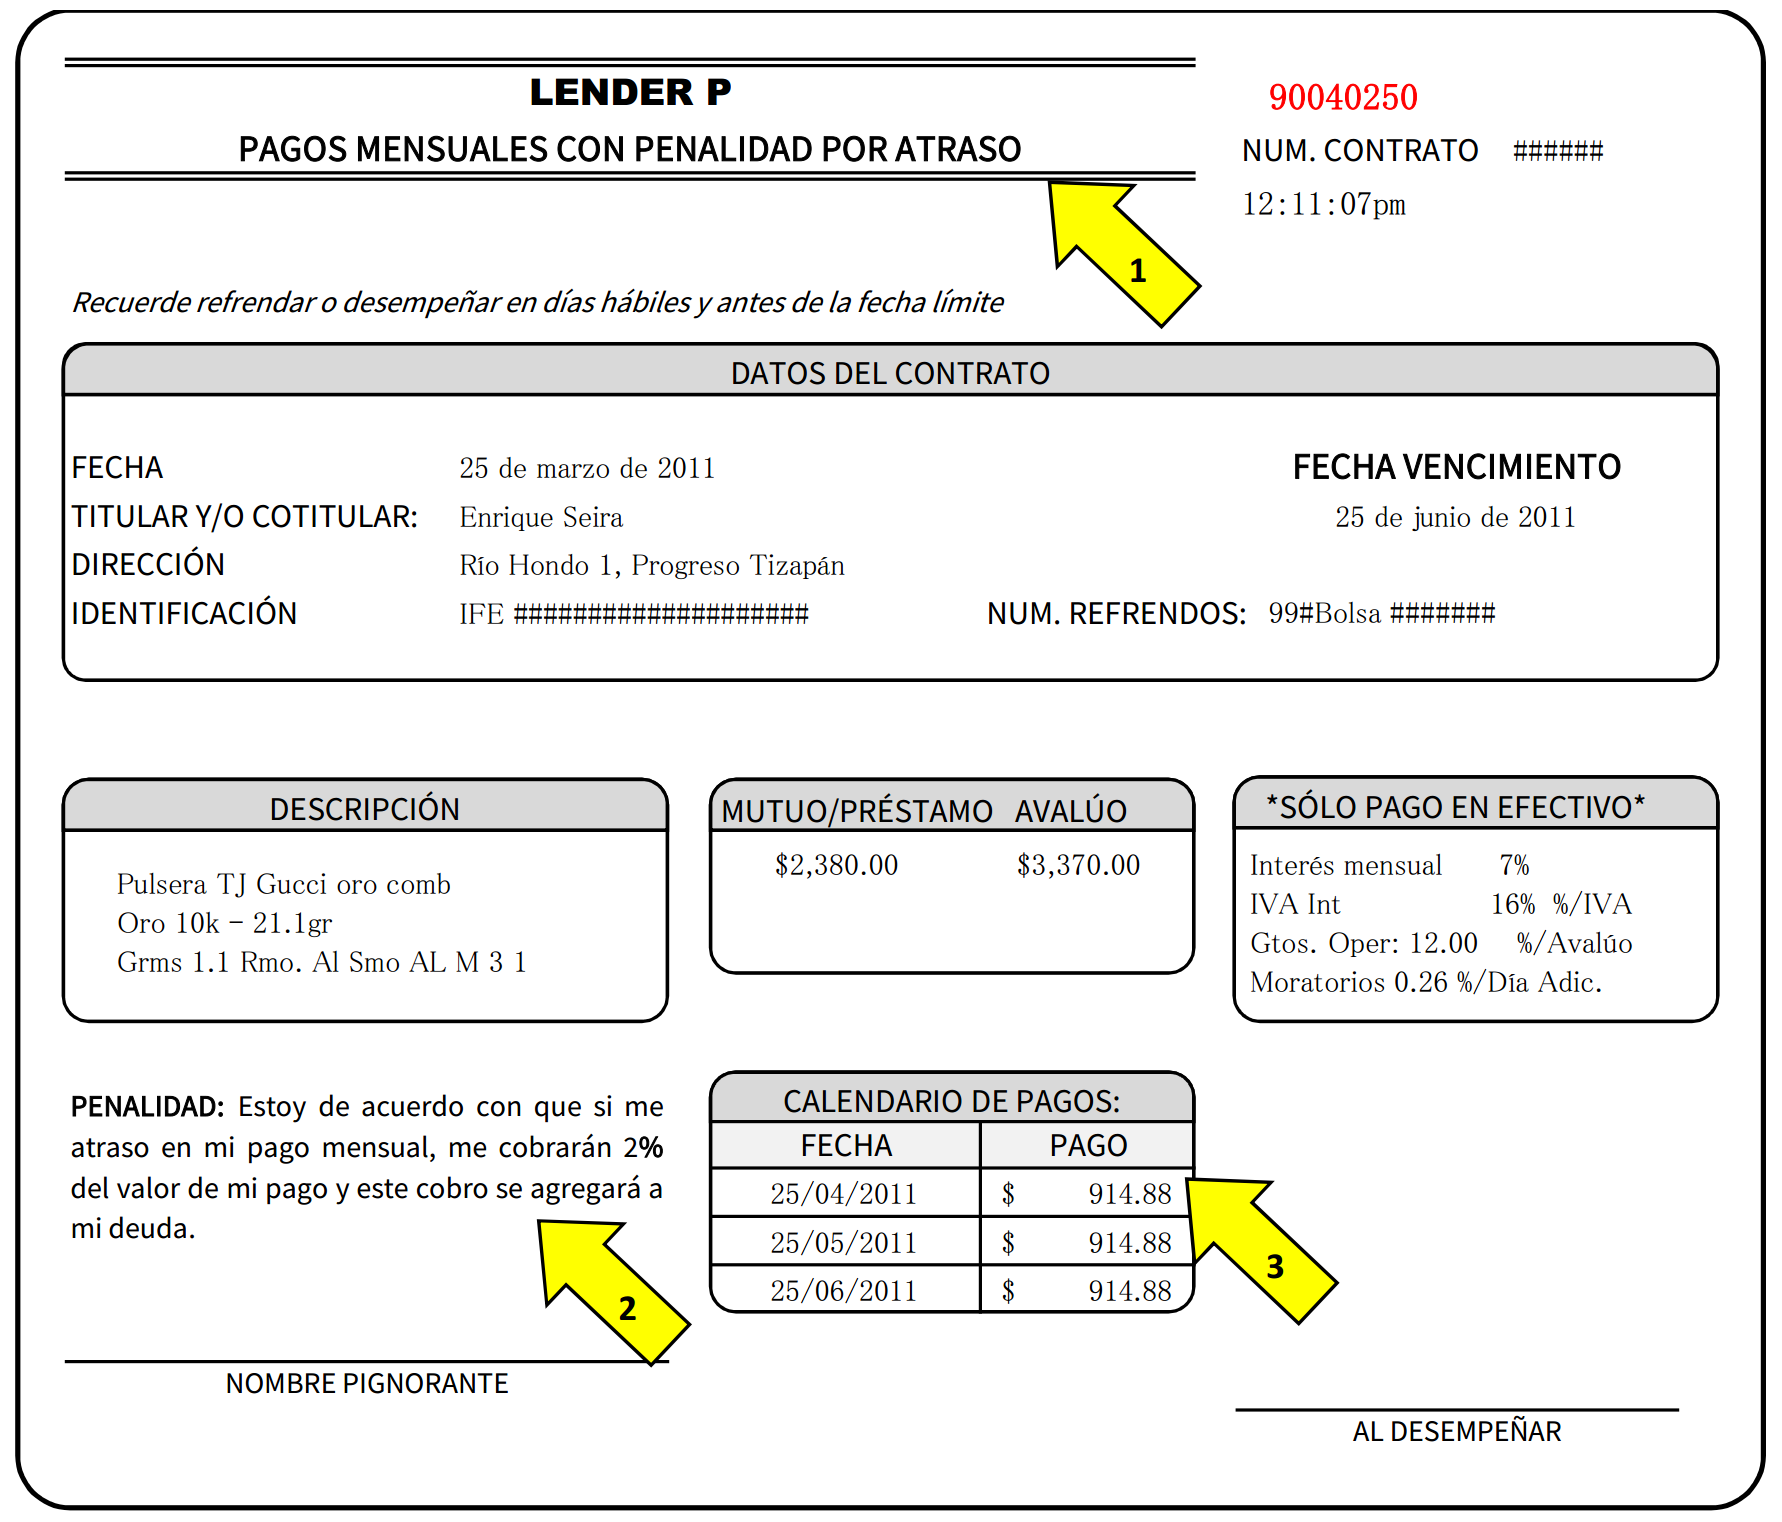
\includegraphics[width=\textwidth]{Figuras/TicketLenderP.png}
    \end{subfigure}
    
    \vspace{3ex}
    \begin{subfigure}{0.65\textwidth}
    \caption{Personal promise signed by client}
        \centering
        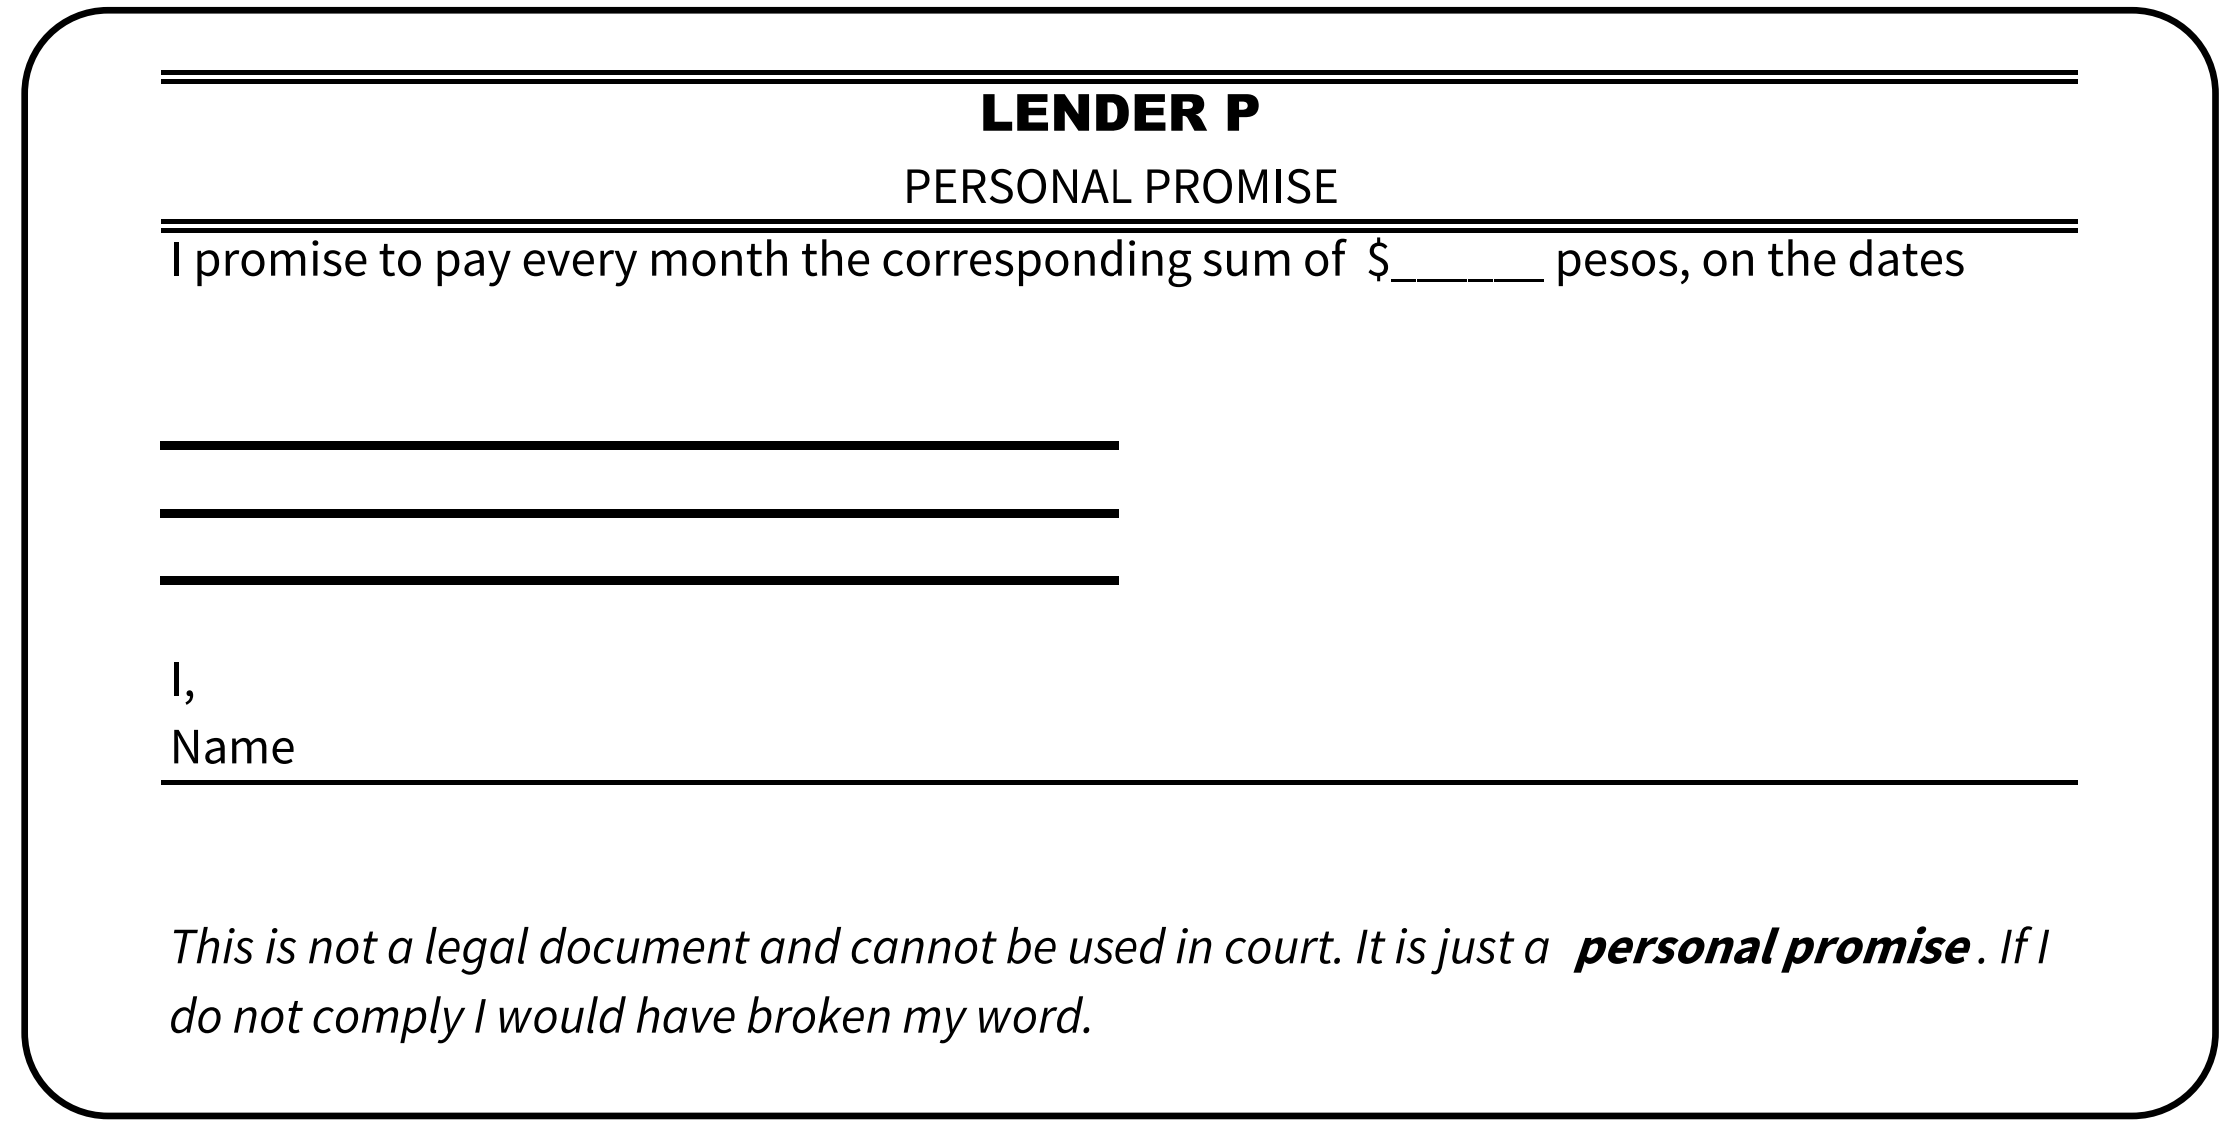
\includegraphics[width=\textwidth]{Figuras/Personal Promise2.png}
    \end{subfigure}
    \end{center}
    \scriptsize
        The top of this figure is a sample receipt that was given to clients that got assigned to the fee-forcing contract (the font and format were changed to protect Lender's P identity). We want to highlight the salience of some items. First the title clearly indicated which contract the client has (arrow 1). Second, in the case of the fee contract it clearly indicates that there is a fee for paying late equivalent to 4\% of the value of the monthly payment (arrow 2). Third, there is a calendar for payments clearly specifying the dates and amounts to pay each month. The bottom panel of the figure shows a ``promise slip'', the paper that those who were assigned (or chose) to the monthly payment with promise had to sign to make the promise salient. It emphasizes that the client is giving his word, and that the promise is not a legal document.
\end{figure}



\subsection{Pictures}

\begin{figure}[H]
     \caption{Some Pawnshops}
    \label{PawnshopPicture}
    \begin{center}
    \begin{subfigure}{0.42\textwidth}
    \caption{Appraiser/tellers inside a pawnshop}
        \centering
        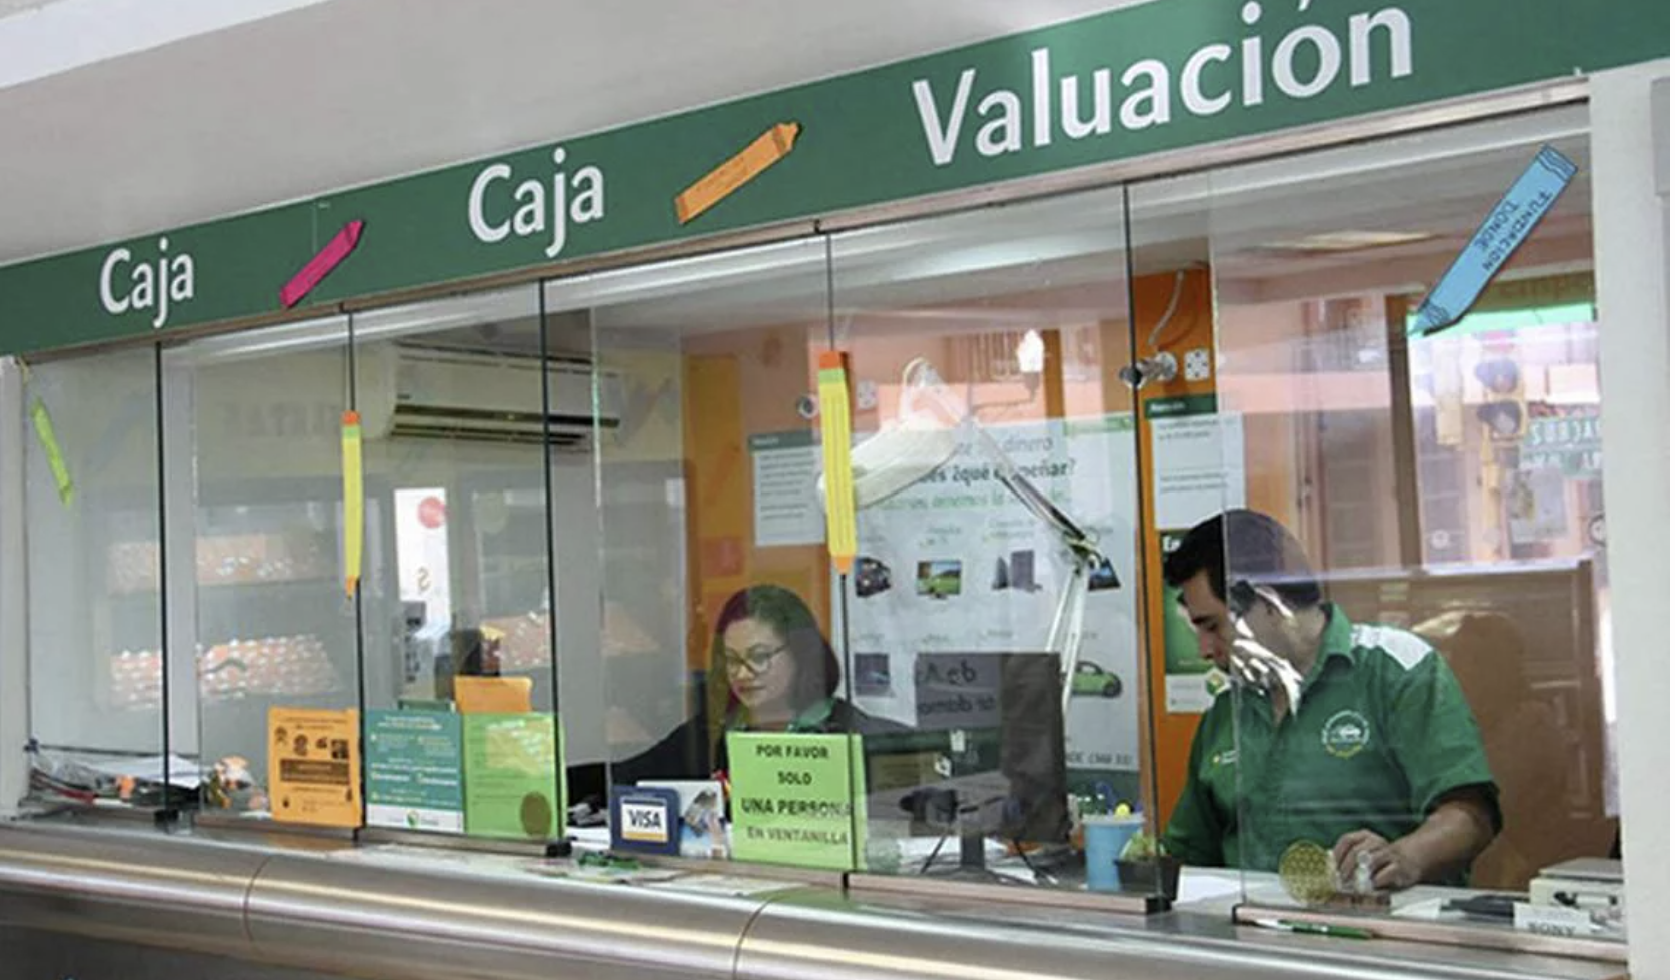
\includegraphics[width=\textwidth]{Figuras/empenio9.png}
    \end{subfigure}
        \begin{subfigure}{0.45\textwidth}
    \caption{Pawnshop}
        \centering
        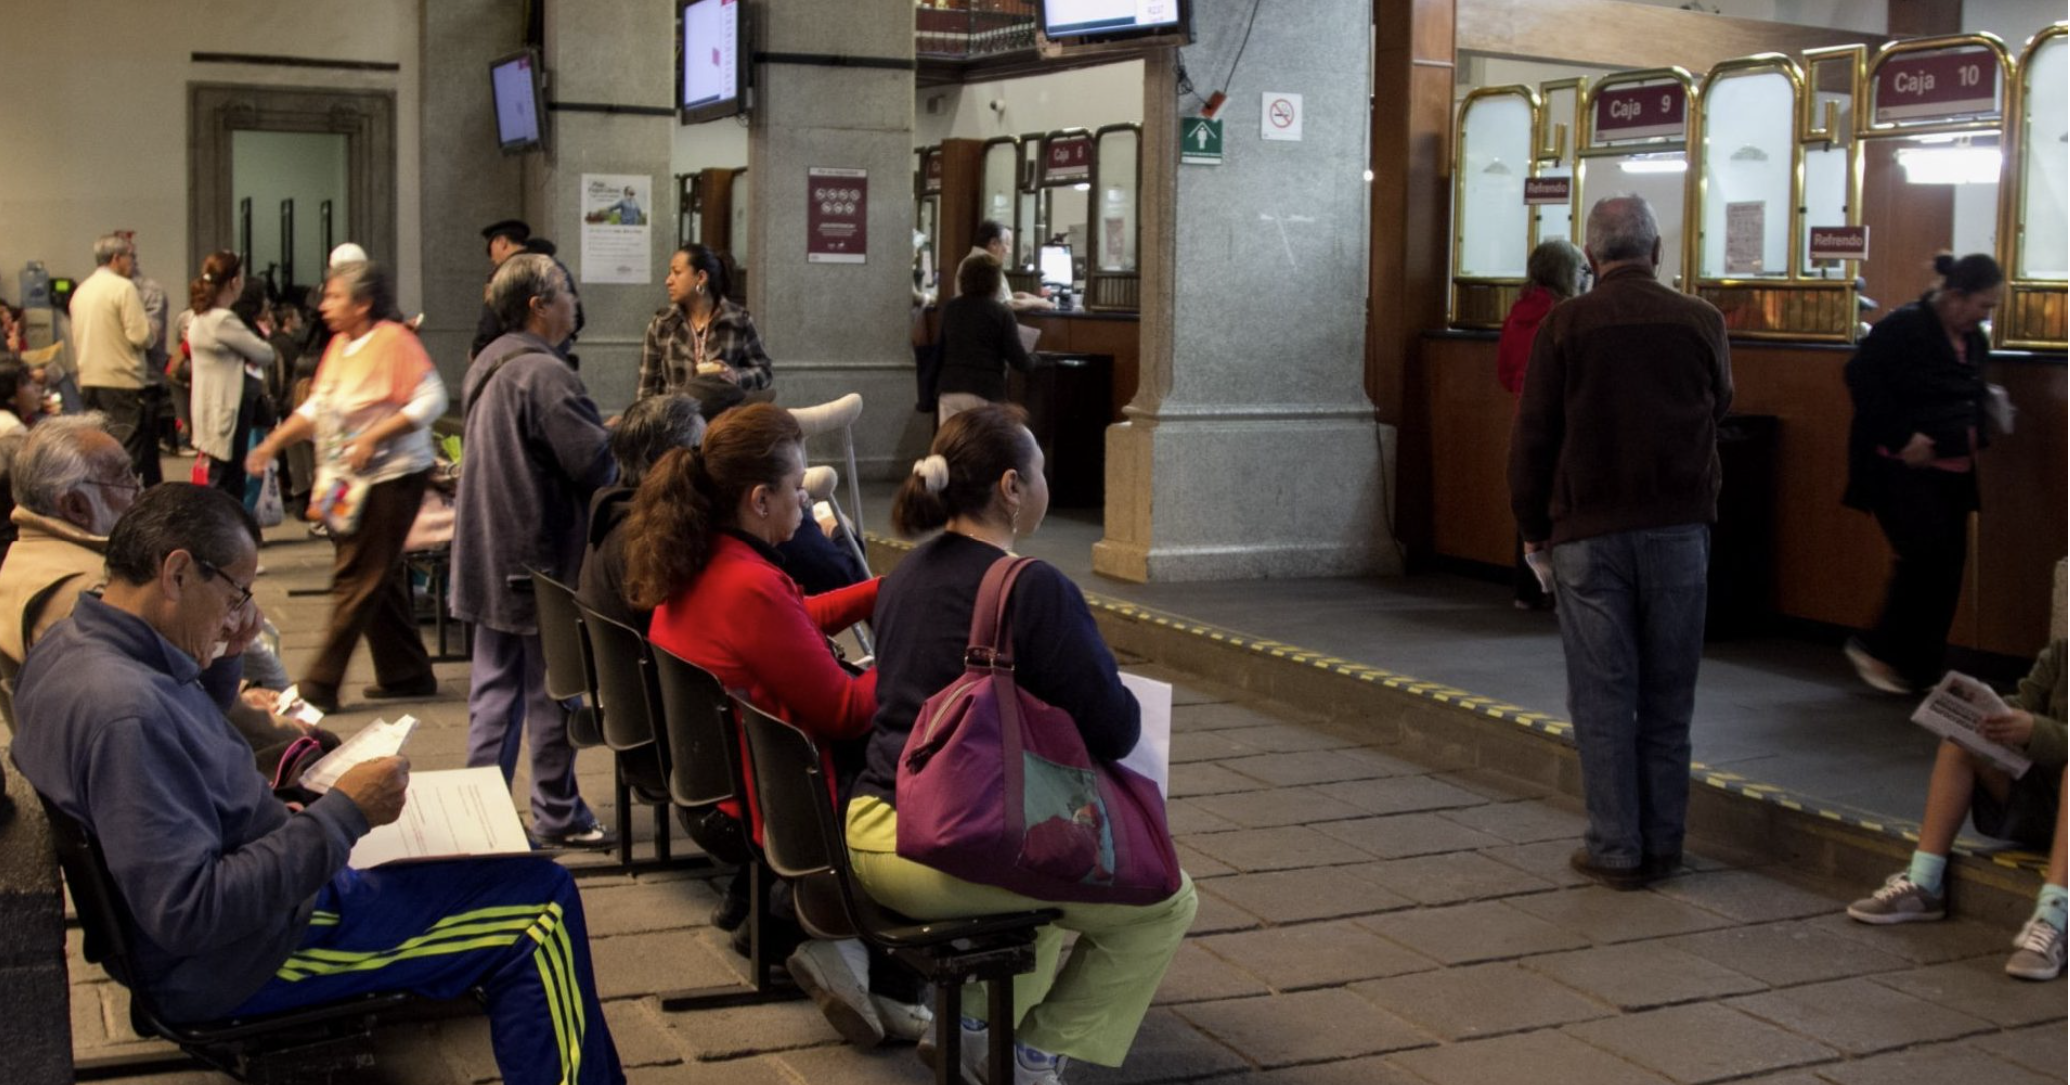
\includegraphics[width=\textwidth]{Figuras/empenio11.png}
    \end{subfigure}
    
        \vspace{3ex}

    \begin{subfigure}{0.45\textwidth}
    \caption{Pawnshop}
        \centering
        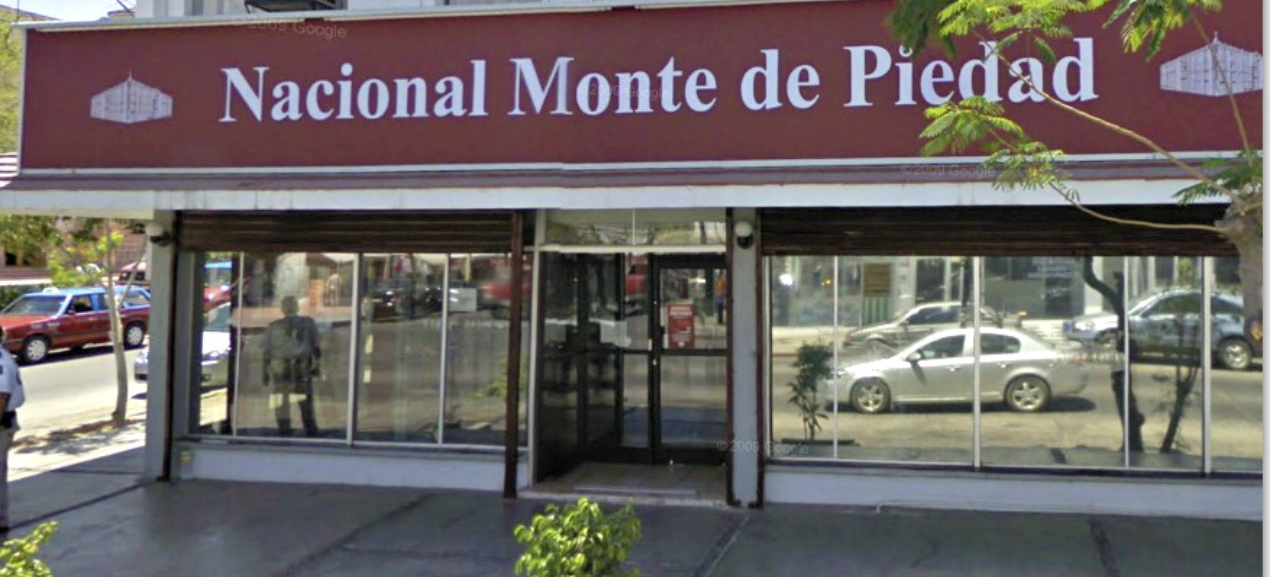
\includegraphics[width=\textwidth]{Figuras/empenio2.png}
    \end{subfigure}
    \begin{subfigure}{0.42\textwidth}
    \caption{Lost pawns which are for sale}
        \centering
        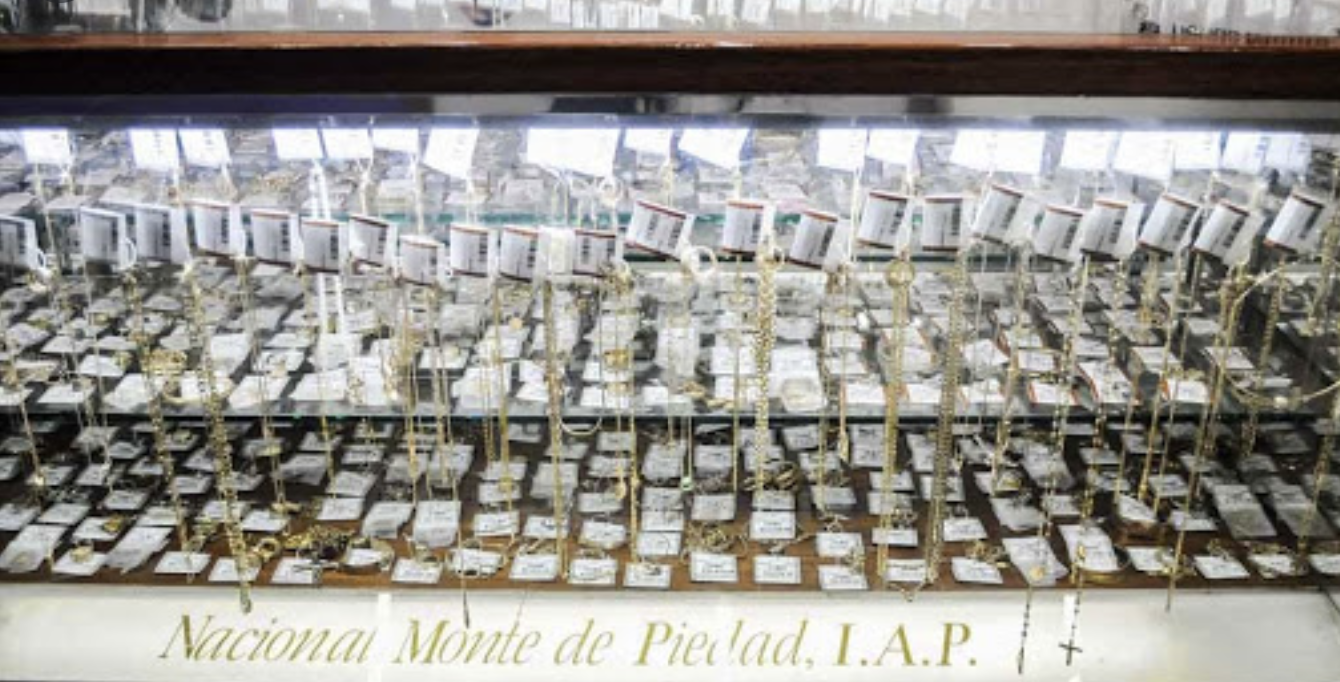
\includegraphics[width=\textwidth]{Figuras/empenio3.png}
    \end{subfigure}
       

    
    \end{center}
    \scriptsize
        This figure  shows pictures of pawnshops in Mexico city. They do not necessarily coincide with Lender P for confidentiality. 
\end{figure}



\vspace{.1in}
\begin{figure}[H]
     \caption{Gold buyers next to pawnshops}
    \label{GoldBuyers}
    \begin{center}
    \begin{subfigure}{.49\textwidth}
    \caption{Gold buyer next to pawnshop 1}
        \centering
        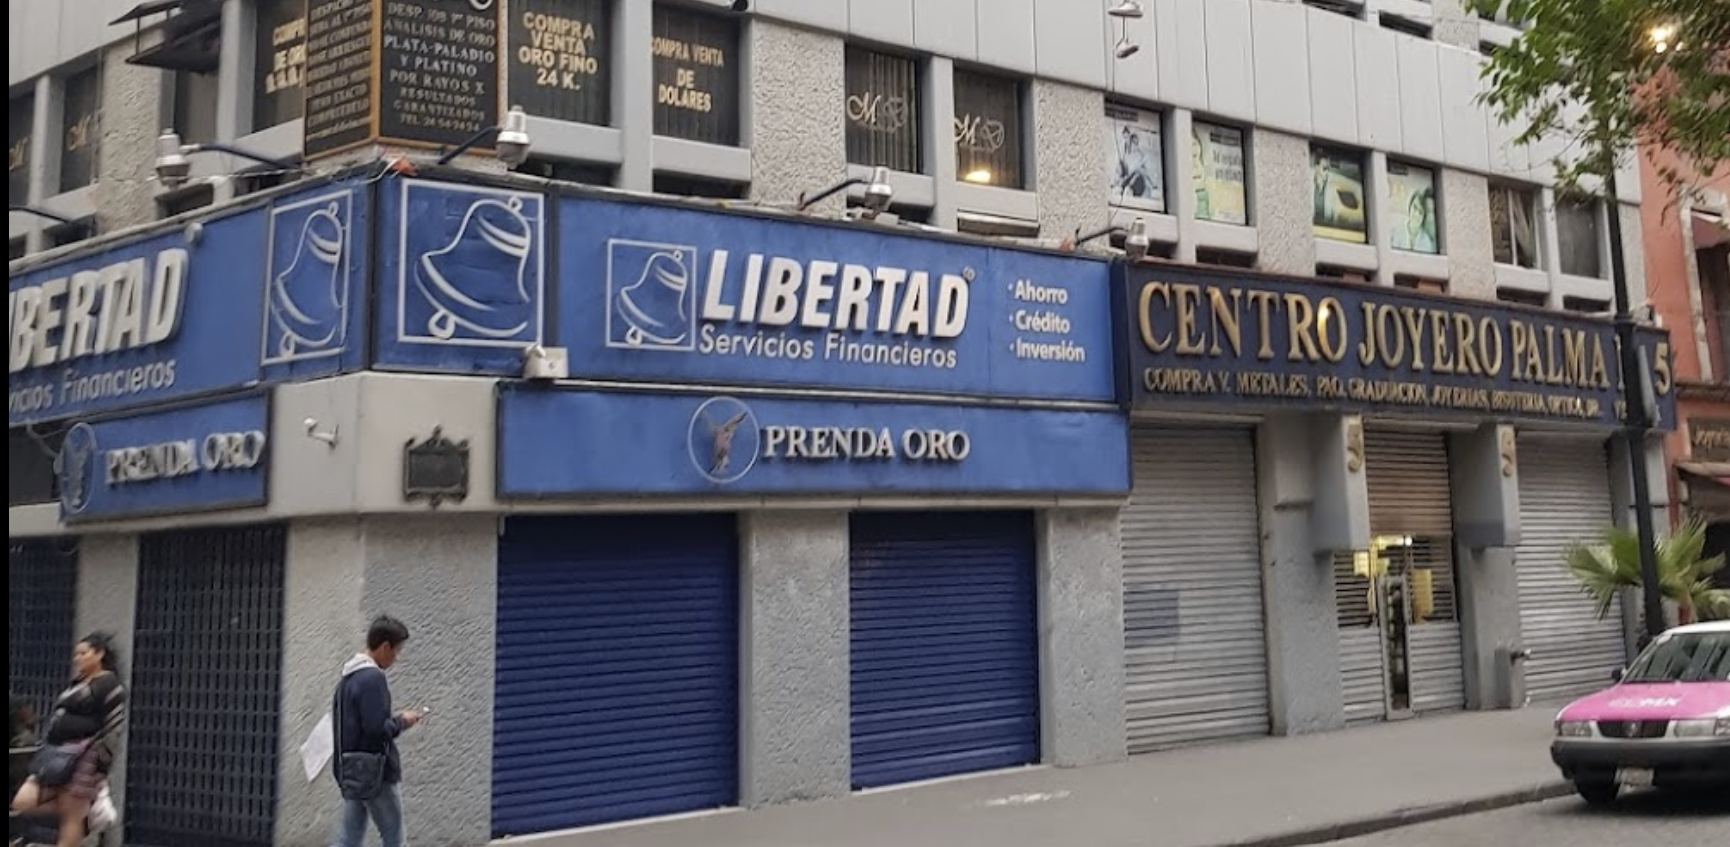
\includegraphics[width=\textwidth]{Figuras/empenio7.png}
    \end{subfigure}
    \begin{subfigure}{.49\textwidth}
    \caption{Gold buyer next to pawnshop 1}
        \centering
        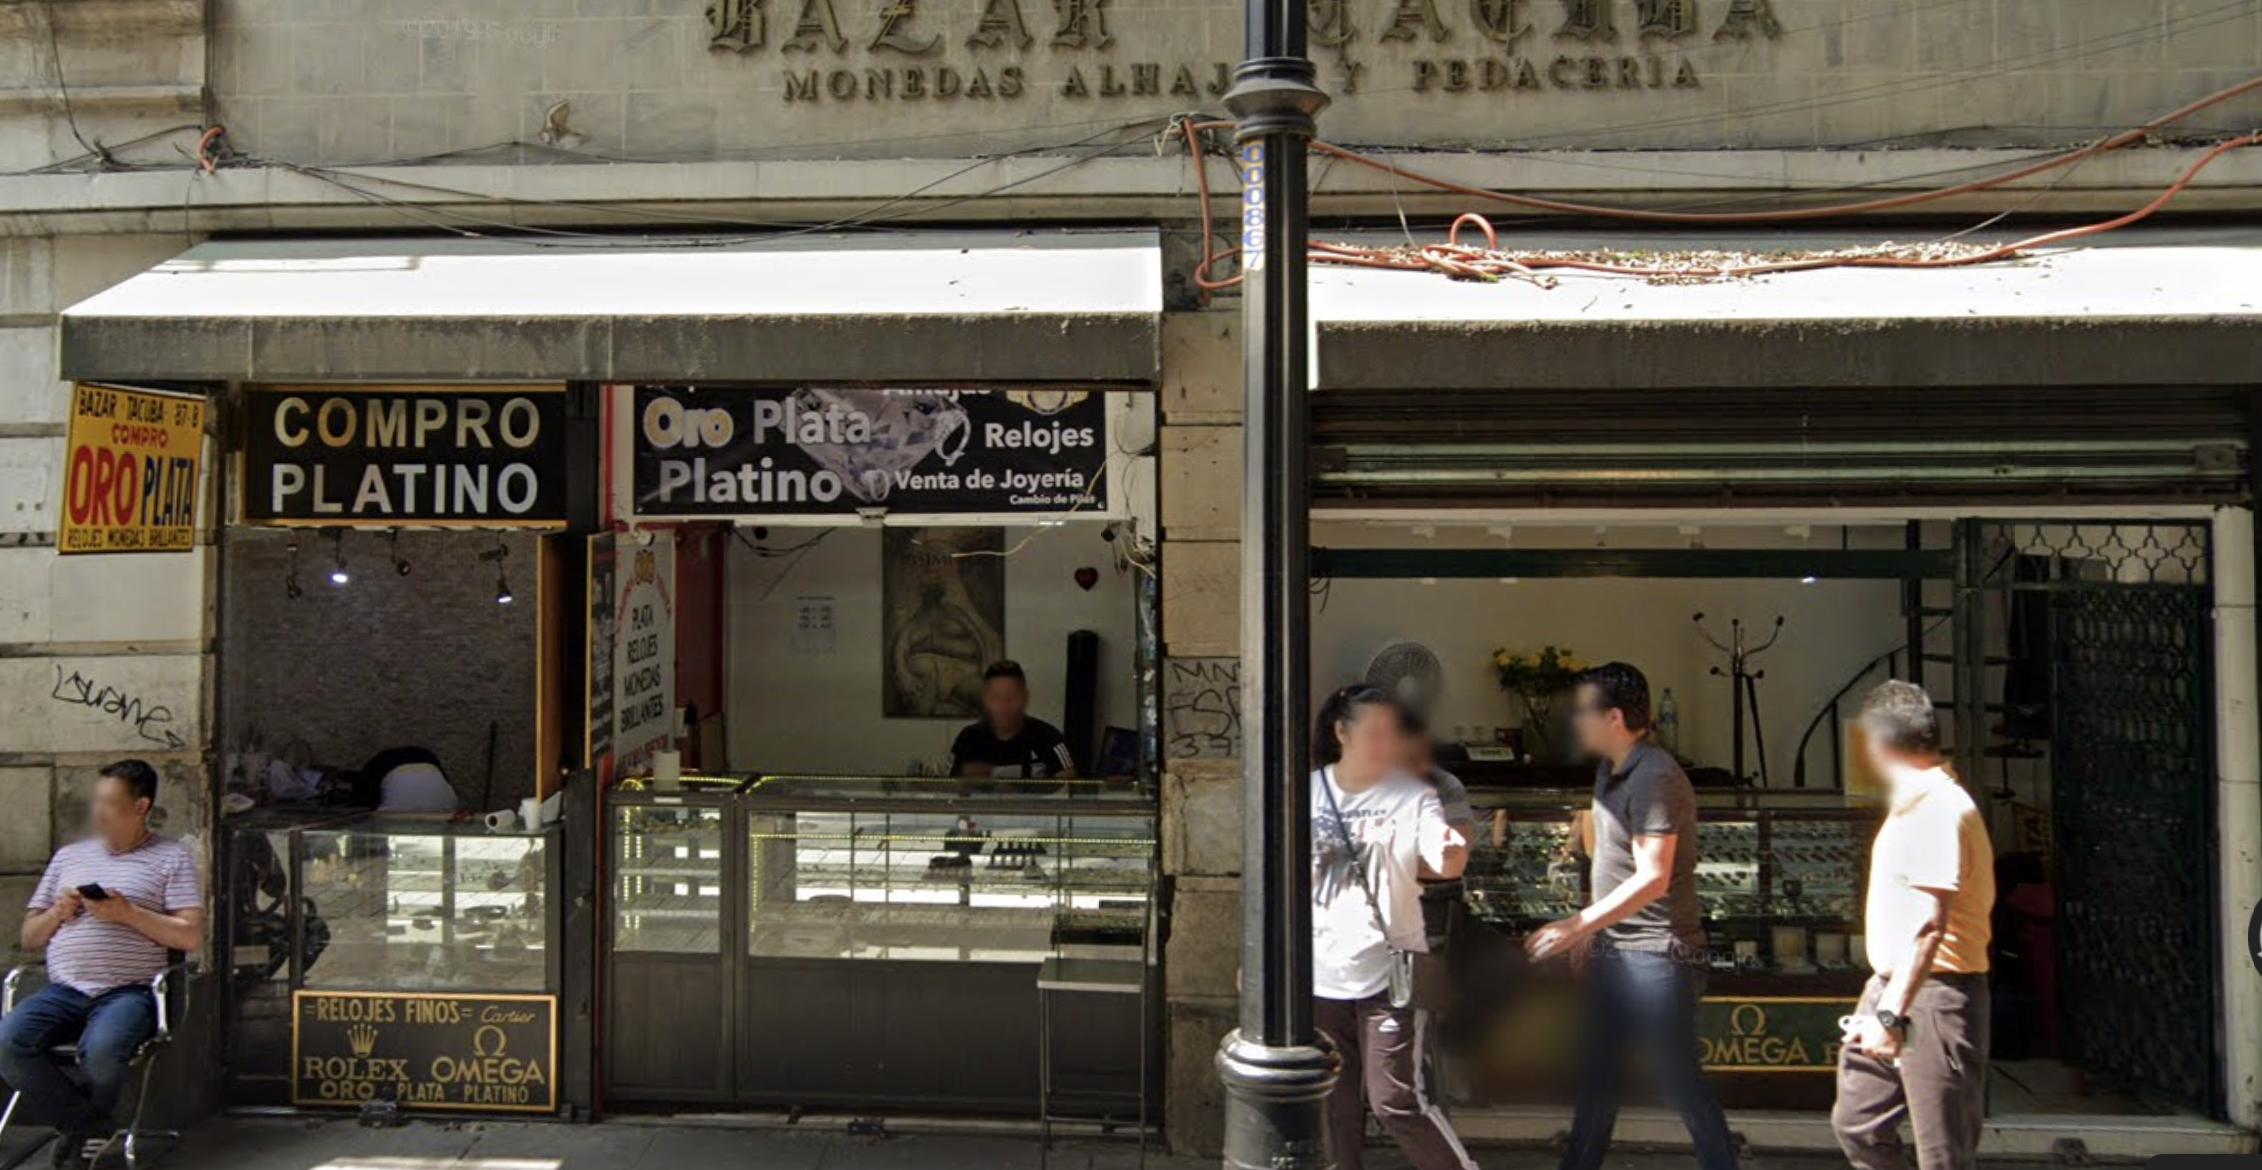
\includegraphics[width=\textwidth]{Figuras/empenio8.png}
    \end{subfigure}
       \vspace{3ex}
       
    \end{center}
    \scriptsize
        This figure shows pictures of gold buyers next to pawnshops in Mexico city. They do not necessarily coincide with Lender P for confidentiality. 
\end{figure}




%\begin{figure}[H]
%        \caption{Booklet with product information}
%    \label{micas}
%    \begin{center}
%        \centering
%        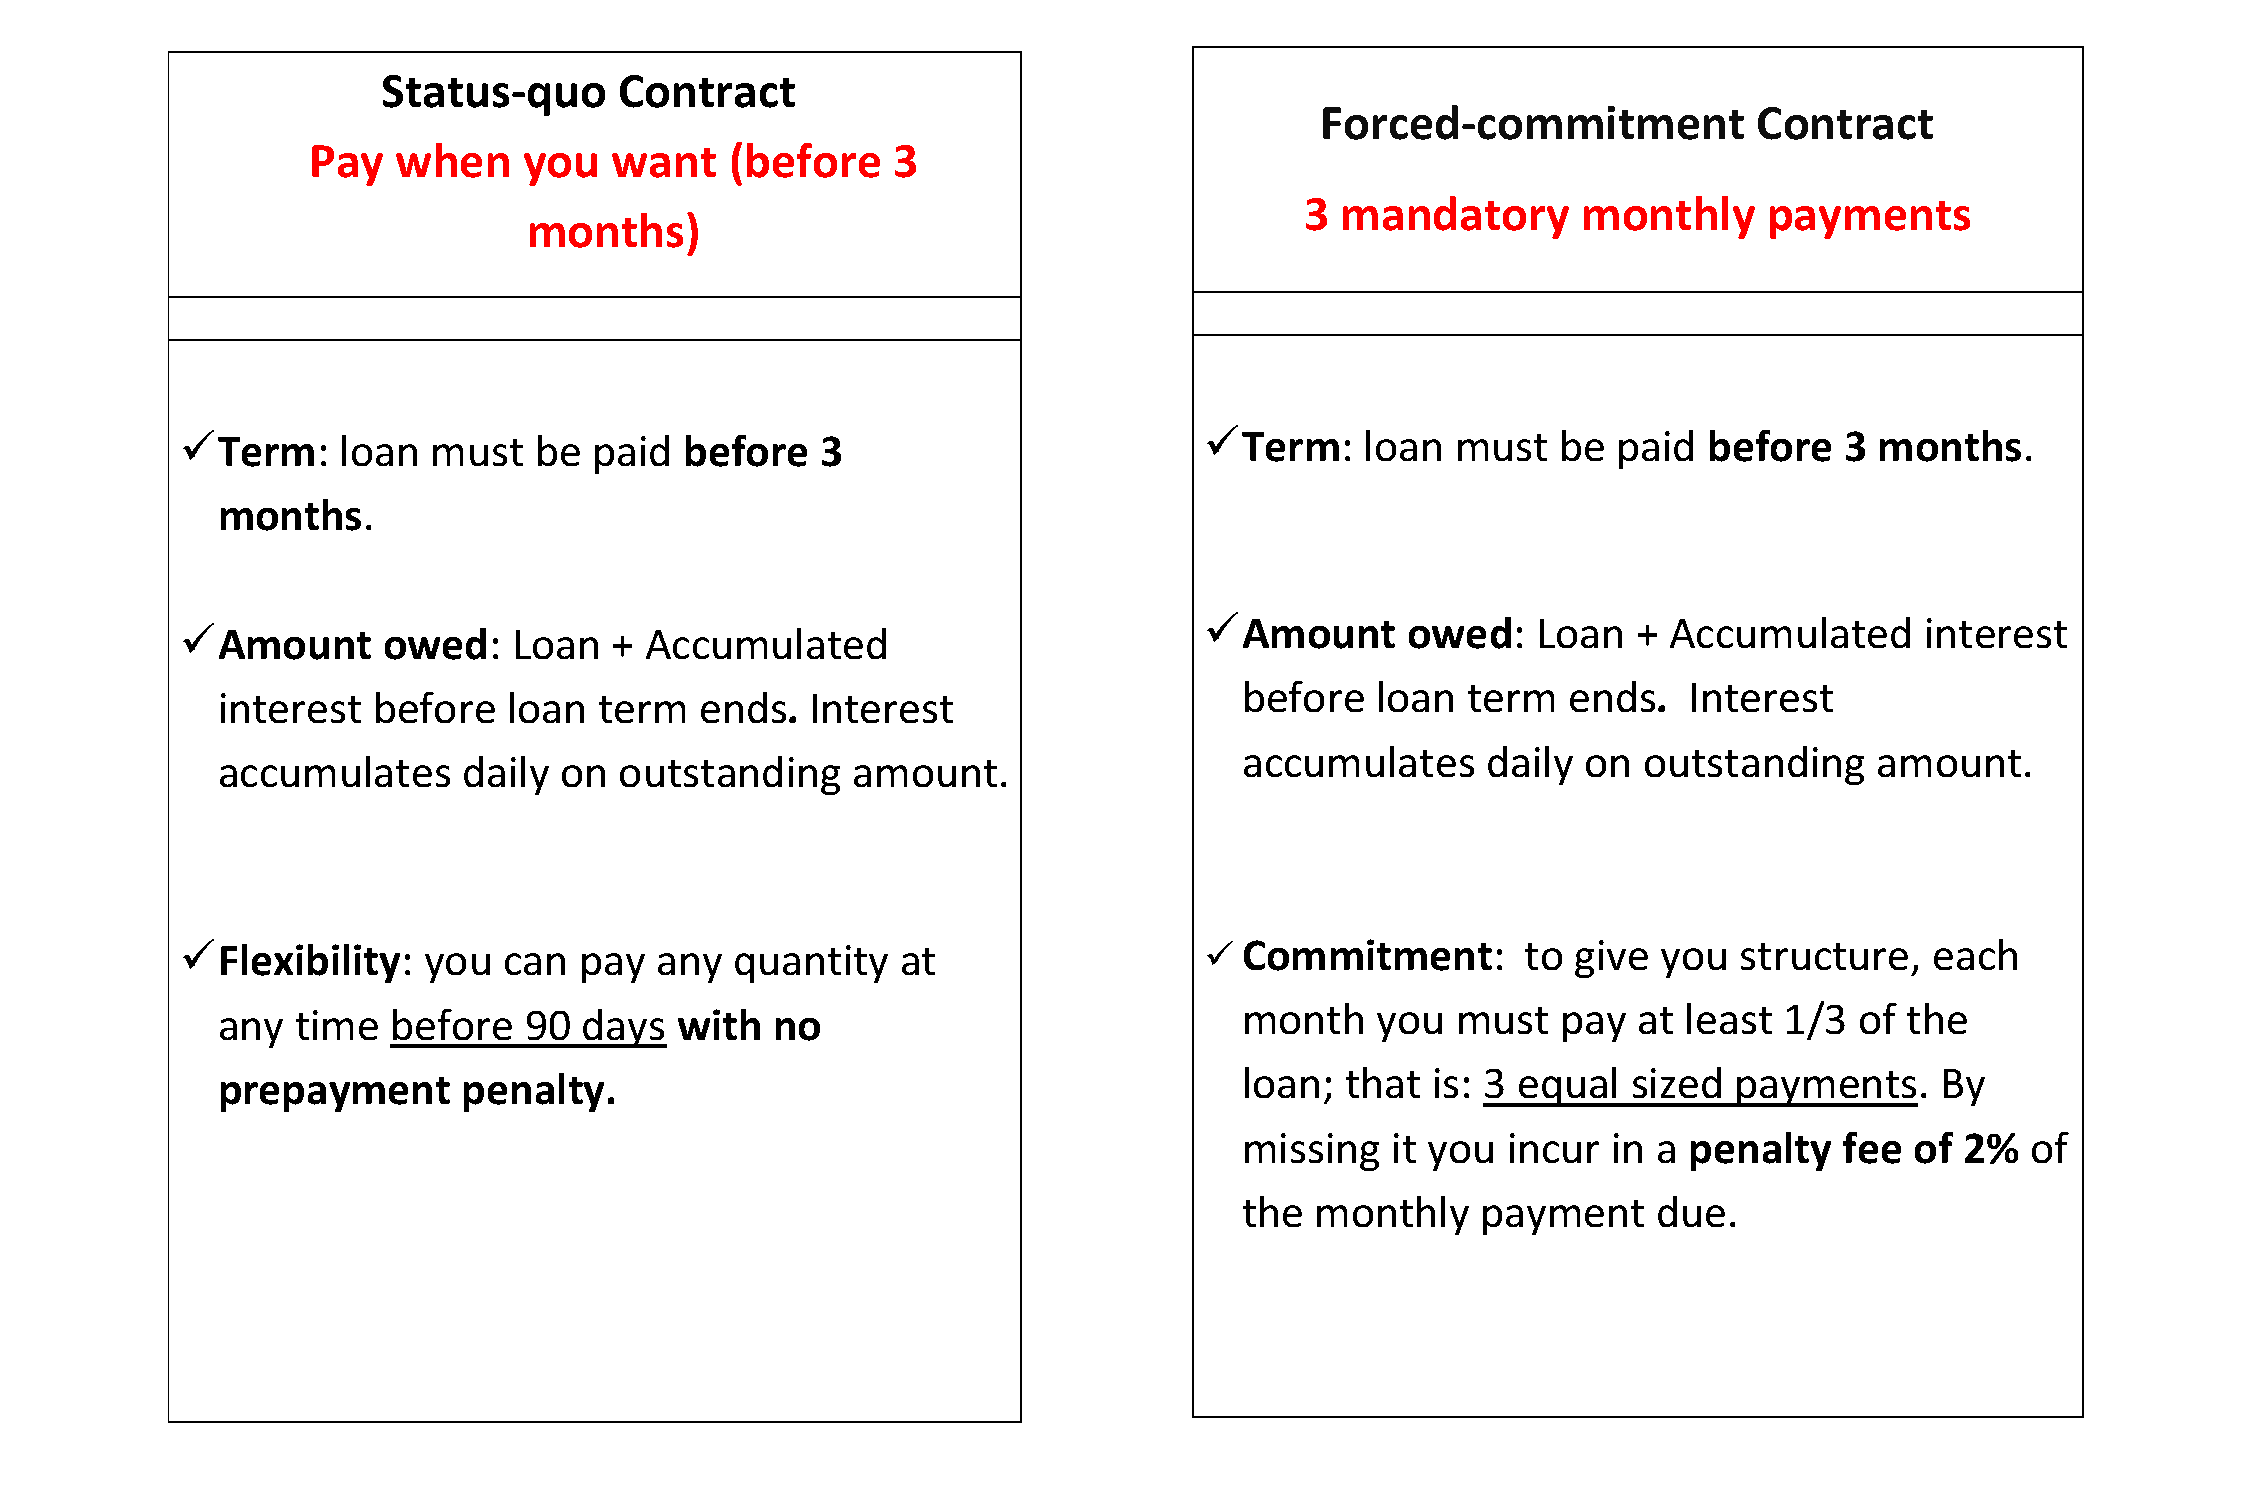
\includegraphics[width=\textwidth]{micas.pdf}
%    \end{center}
%     \footnotesize \textit{Notes: } 
%      \footnotesize{ }
%\end{figure}


%\begin{figure}[H]
%     \caption{Booklet with product information translated}
%    \label{booklet_translate2}
%    \begin{center}
%    \begin{subfigure}{.9\textwidth}
%        \centering
%        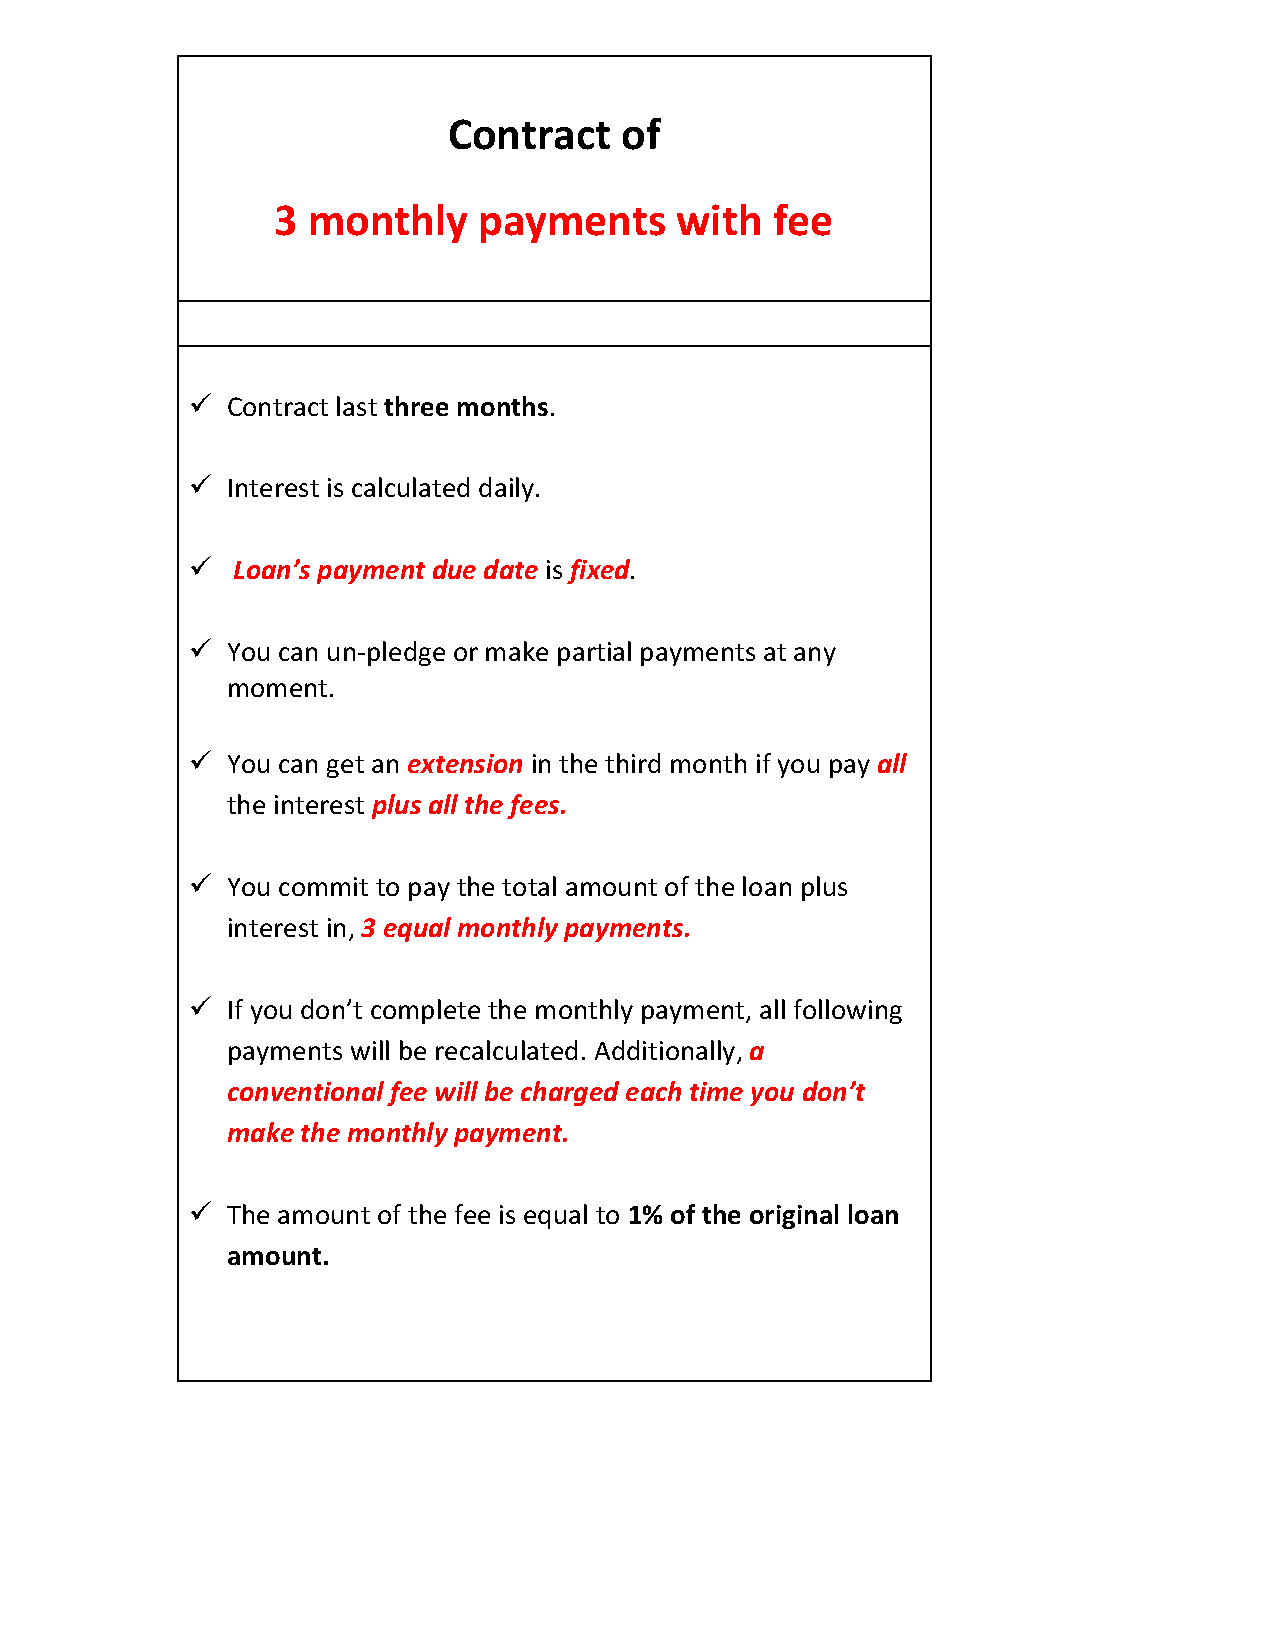
\includegraphics[width=\textwidth]{Figuras/MP_F.pdf}
%    \end{subfigure}
    %\begin{subfigure}{0.55\textwidth}
    %   \centering
    %  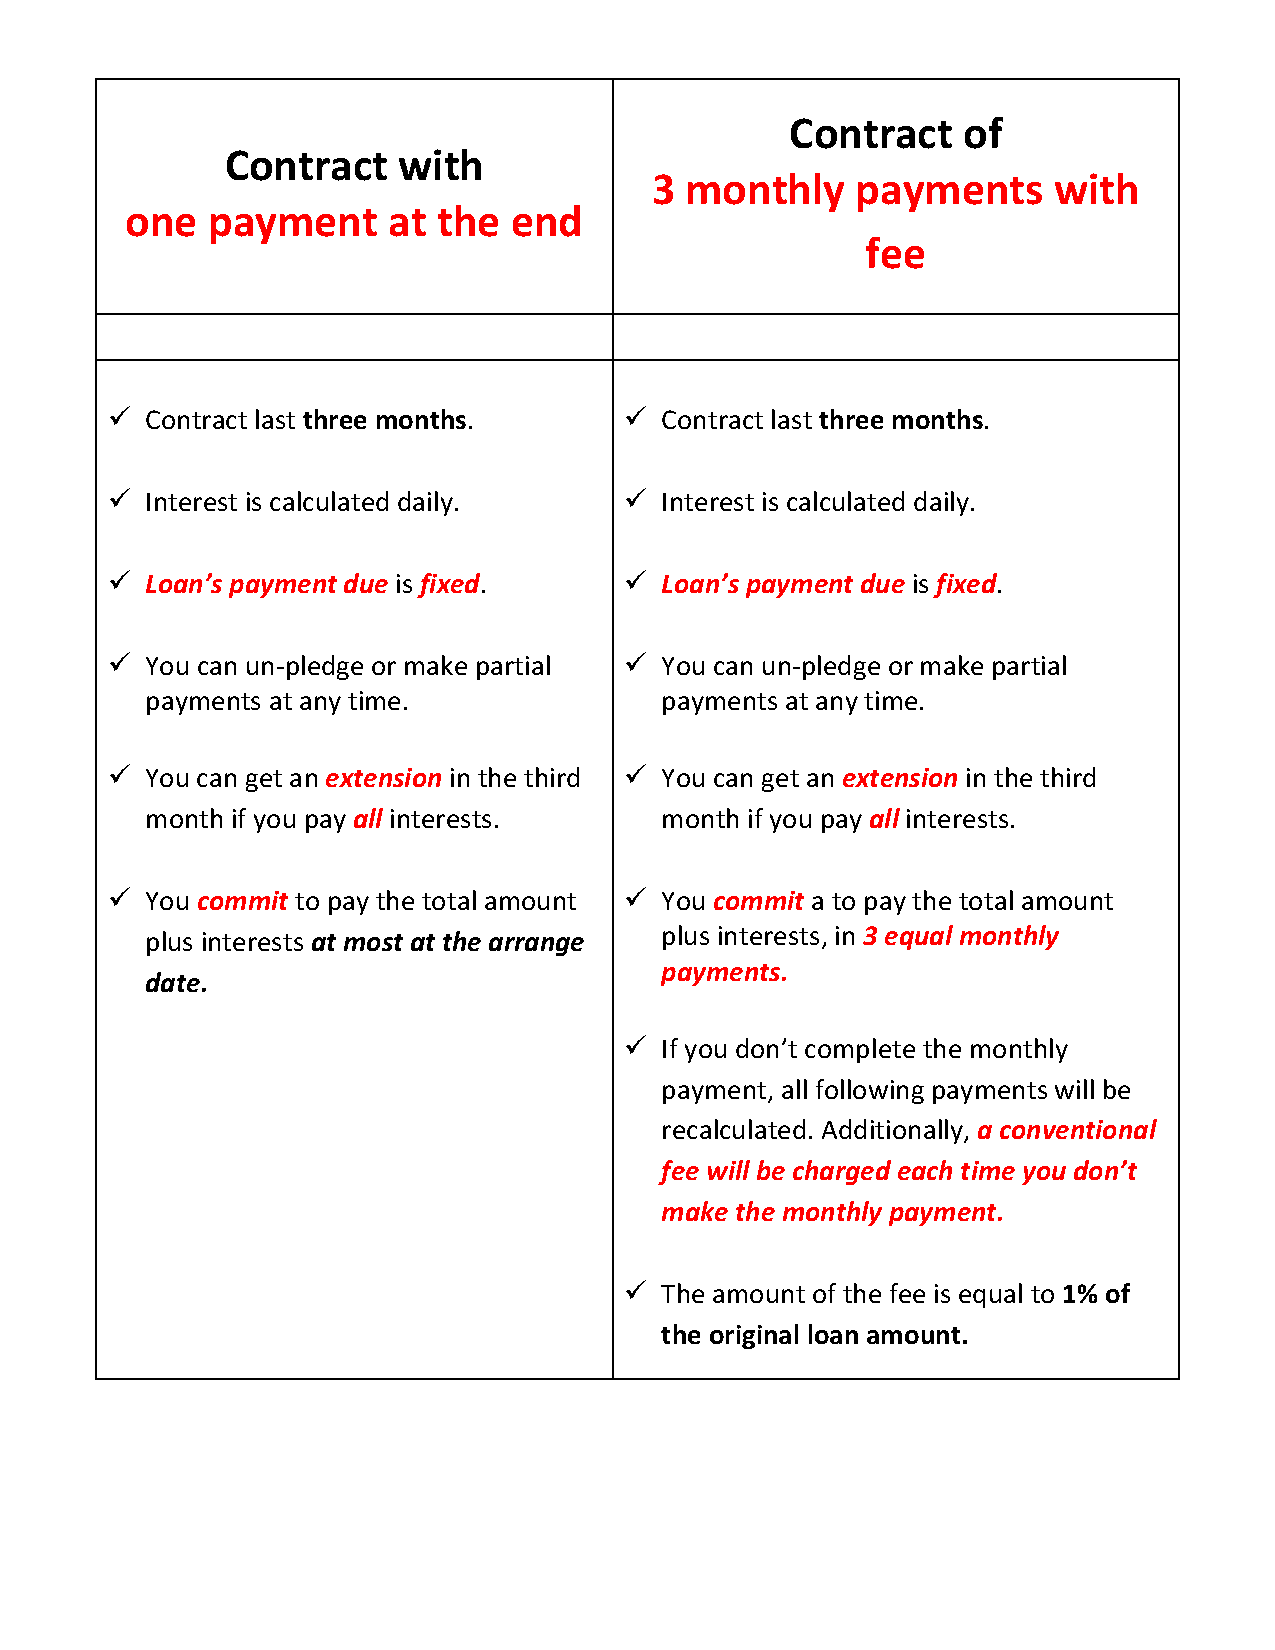
\includegraphics[width=\textwidth]{Figuras/MP_2.pdf}
    %\end{subfigure}
%    \end{center}
%\end{figure}



\subsection{Surveys}


\begin{table}[H]
\caption{Survey's non-response balance}
\label{balance_response}
\begin{center}
\scriptsize{% Table generated by Excel2LaTeX from sheet 'balance_response'
\begin{tabular}{lcccc|ccc}
\toprule
      &       & \multicolumn{3}{c|}{Panel A : Entry Survey} & \multicolumn{3}{c}{Panel B : Exit Survey} \\
\midrule
\midrule
      & Overall & No Response & Response & p-value & No Response & Response & p-value \\
\midrule
\midrule
Loan amount  & 2145.46 & 2262.14 & 2145.46 & 0.08  & 2157.15 & 2367.62 & 0.17 \\
      & (31.81) & (59.21) & (35.45) &       & (30.93) & (154.83) &  \\
Monday & 0.18  & 0.18  & 0.18  & 0.95  & 0.18  & 0.19  & 0.71 \\
      & (0.02) & (0.03) & (0.02) &       & (0.02) & (0.04) &  \\
Number of branch-day pawns & 33.03 & 32.13 & 33.33 & 0.61  & 32.83 & 35.66 & 0.51 \\
      & (1.04) & (2.08) & (1.2) &       & (1.07) & (4.18) &  \\
\midrule
Obs   & 13444 & 3007  & 10437 &       & 12539 & 905   &  \\
\bottomrule
\bottomrule
\end{tabular}%
}
\end{center}
 \scriptsize This table shows whether the means of variables in the administrative dataset are different for those that respond the baseline survey vs those that do not. We use this as an assessment of external validity. Internal validity is guaranteed because the baseline survey was implemented before treatment assignment and therefore response rates are orthogonal to treatment assignments. Panel A studies the baseline survey, while Panel B focuses on the exit survey. The columns labeled ``p-values'' report p-values for the test that the means of the respective variable are the same for those that responded did not respond the survey.
%\textit{Do file: } \texttt{balance\_response.do}
\end{table}


\afterpage{
\begin{table}[H]
\caption{Baseline survey}
\label{baseline_survey}
\begin{center}
\scriptsize{% Table generated by Excel2LaTeX from sheet 'transcribed'
\begin{tabular}{cl}
\toprule
      & \textbf{Baseline Survey} \\
\midrule
\midrule
1     & \textbf{Your pawn was:} \\
      & (a) Inherite, (b) a gift, (c) bought by me, (d) lend to me, (e) other \_\_\_\_\_\_\_\_\_\_\_\_ \\
2     & \textbf{Mark with an "X" in the line below how likely is that you recover your pawn. } \\
      & \textbf{Where 0 is impossible and 100 is completely certain} \\
3     & \textbf{How much do you think the item you plan to pawn is worth?       \_\_\_\_\_\_\_\_\_\_\_\_\_\_ pesos} \\
4     & \textbf{Gender      } \\
5     & \textbf{Age} \\
6     & \textbf{Civil Status } \\
      & (a) married, (b) single, (c) divorced, (d) widowed \\
7     & \textbf{Work status} \\
      & (a) employed, (b) own business, (c) houseshores, (d) don't work, (e) retired, (f) study \\
8     & \textbf{Education} \\
      & (a) no formal education, (b) primary, (c) middle school, (d) highschool, (e) more than highschool \\
9     & \textbf{In the last month, did a friend or family member asked you for money?} \\
      & (a) yes  (b) no \\
10    & \textbf{What would you like to have: 100 pesos tomorrow or 150 pesos in one month?} \\
11    & \textbf{How often do you feel stressed by your economic situation?} \\
      & (a) always, (b) very often, (c) sometimes, (d) never \\
12    & \textbf{What is the main reason you want to pawn?} \\
      & (a) Need the money because somebody in my family lost his/her job \\
      & (b) Need the money to pay for a sickness in the family \\
      & (c) Need the money for an urgent expense \\
      & (d) Need the money for some non urgent expense. \\
13    & \textbf{How stressed do you feel from the situation that led to to pawn?} \\
      & (a) very stressed, (b) somwhat stressed, (c) a little stressed, (d) not stressed  \\
14    & \textbf{In 3 months, I expect to have a  \_\_\_\_\_\_\_\_\_\_\_\_\_\_\_\_ situation} \\
      & (a) better, (b) similar,  (c) worse \\
15    & \textbf{Have you panwned before?} \\
      & (a) yes  (b) no \\
16    & \textbf{How many times have you pawned on a Lender P branch?} \\
      & (a) NO\_\_\_    (b)  1-2 times \_\_\_    (c) 3-5 times\_\_\_\_   (d) More than 5\_\_\_\_ \\
17    & \multicolumn{1}{p{54.91em}}{\textbf{If you are saving money and a family member wants to use it for something }} \\
      & \multicolumn{1}{p{54.91em}}{(a) I would only give him the money for an urgent expenze} \\
      & \multicolumn{1}{p{54.91em}}{(b) I would give him the money even if it was not an urgent expense} \\
      & \multicolumn{1}{p{54.91em}}{(c) I would not give him/her the money regardless} \\
      & \multicolumn{1}{p{54.91em}}{(d) No one would ask me for my money} \\
18    & \textbf{Do you make an expenses budget for the month ahead of time?} \\
      & (a) always, (b) very often, (c) sometimes, (d) never \\
19    & \multicolumn{1}{p{54.91em}}{\textbf{Do you have other items you could pawn?}} \\
      & (a) yes  (b) no \\
20    & \textbf{Do you have savings?} \\
      & (a) yes  (b) no \\
21    & \textbf{Do you participate in a ROSCA?} \\
      & (a) yes  (b) no \\
22    & \textbf{Is it common that family or friends ask for money?} \\
      & (a) yes  (b) no \\
23    & \textbf{How much did you spend to come to the branch today?    \$\_\_\_\_\_\_\_\_\_\_\_\_\_\_ pesos} \\
24    & \textbf{How much time does it usually take to come to this branch?    \_\_\_\_\_\_\_\_\_\_\_} \\
25    & \textbf{How much does your family spend in a normal week?   \$\_\_\_\_\_\_\_\_\_\_\_\_\_\_ pesos} \\
26    & \textbf{How much do you manage to save in a normal week?   \$\_\_\_\_\_\_\_\_\_\_\_\_\_\_ pesos} \\
27    & \textbf{Does it happen to you that you spend more than you wanted because you fall into temptation?} \\
      & (a) never, (b) almost never, (c) sometimes, (d) very often \\
28    & \textbf{In the last 6 months, has it happened that at some point you lacked money to pay} \\
      & (a) rent?    (b) food    (c)food   (d) medicine  (e) electricity   (f) heating   (g) telephone    (i) water \\
29    & \textbf{What would you like to have: 100 pesos in 3 months or 150 pesos in four months?} \\
30    & \textbf{Would you like to receive (free) reminders for upcomming payments?} \\
      & (a) yes  (b) no \\
\bottomrule
\end{tabular}%
}
\end{center}
\end{table}
}


\begin{comment}
\begin{table}[H]
\caption{Reincidence SS}
\label{tab_reincidence}
\begin{center}
\scriptsize{% Table generated by Excel2LaTeX from sheet 'tab_reincidence'
\begin{tabular}{lccccc}
\toprule
Variable & Obs   & Mean  & Std. Dev. & Min   & Max \\
\midrule
\midrule
Number of visits & 26179 & 1.72  & 1.27  & 1     & 7 \\
Received more one treatment arm & 26179 & 0.23  & 0.42  & 0     & 1 \\
Number of arms & 26179 & 1     & 1.06  & 0     & 5 \\
Reincidence & 16470 & 0.29  & 0.45  & 0     & 1 \\
Same product of reincidence & 16470 & 0.02  & 0.13  & 0     & 1 \\
Number of visits $<$ 75 days & 26179 & 2.1   & 1.5   & 1     & 7 \\
Received more one treatment arm $<$ 75 days & 26179 & 0.22  & 0.41  & 0     & 1 \\
Number of arms  $<$ 75 days & 26179 & 0.97  & 1.01  & 0     & 5 \\
Chose same treatment arm & 1066  & 0.45  & 0.5   & 0     & 1 \\
\bottomrule
\bottomrule
\end{tabular}%
}
\end{center}
 \scriptsize
%\textit{Do file: } \texttt{tab\_reincidence.do}
\end{table}


\begin{table}[H]
\caption{Summary statistics (exit survey)}
\label{SS_exit}
\begin{center}
\scriptsize{% Table generated by Excel2LaTeX from sheet 'SS'
\begin{tabular}{lccccccc}
\toprule
\multicolumn{8}{c}{Exit Survey Data} \\
\midrule
\midrule
      &       &       & \multicolumn{2}{c}{No Choice } & \multicolumn{2}{c}{Choice} &  \\
\midrule
\midrule
      & Overall & Control & Fee   & Promise & Fee   & Promise & p-value \\
\midrule
      & \multicolumn{7}{c}{Panel A: Outcomes} \\
\midrule
\midrule
Will reincide & 0.94  & 0.96  & 0.95  & 0.96  & 0.94  & 0.92  & 0.6 \\
      & (0.01) & (0.01) & (0.02) & (0.02) & (0.02) & (0.03) &  \\
Very satisfied & 0.34  & 0.36  & 0.32  & 0.33  & 0.33  & 0.36  & 0.95 \\
      & (0.02) & (0.05) & (0.05) & (0.05) & (0.04) & (0.04) &  \\
Better econ situation & 0.42  & 0.53  & 0.29*** & 0.35** & 0.44  & 0.47  & 0.02 \\
      & (0.03) & (0.06) & (0.05) & (0.06) & (0.05) & (0.04) &  \\
Choose frequent payment & 0.63  & 0.65  & 0.58  & 0.58  & 0.58  & 0.77** & 0 \\
      & (0.02) & (0.05) & (0.05) & (0.06) & (0.04) & (0.03) &  \\
\midrule
      & \multicolumn{7}{c}{Panel B: Balance} \\
\midrule
\midrule
Loan amount  & 1957.72 & 1940.41 & 1926  & 2006.83 & 2002.97 & 1892.54 & 0.98 \\
      & (67.84) & (160.03) & (150.89) & (187.56) & (114.96) & (157.83) &  \\
Woman & 0.71  & 0.69  & 0.72  & 0.77  & 0.66  & 0.73  & 0.58 \\
      & (0.02) & (0.05) & (0.06) & (0.05) & (0.05) & (0.04) &  \\
Age   & 43.98 & 42.84 & 46.27 & 43.82 & 44.57 & 42.24 & 0.29 \\
      & (0.59) & (1.33) & (1.74) & (1.1) & (0.99) & (1.16) &  \\
Subjective value & 3166.31 & 3448.99 & 3182.11 & 3049.88 & 3074.69 & 3081.52 & 0.85 \\
      & (120.82) & (288.38) & (286.2) & (303.87) & (210.79) & (296.63) &  \\
Has pawn before & 0.88  & 0.84  & 0.9   & 0.87  & 0.95** & 0.8   & 0.01 \\
      & (0.02) & (0.05) & (0.03) & (0.05) & (0.02) & (0.05) &  \\
Subj. pr. of recovery & 95.35 & 94.5  & 94.84 & 96.6  & 95.06 & 95.87 & 0.82 \\
      & (0.56) & (1.4) & (1.21) & (1.5) & (1.01) & (1.09) &  \\
+High-school & 0.66  & 0.72  & 0.63  & 0.65  & 0.67  & 0.64  & 0.84 \\
      & (0.03) & (0.06) & (0.06) & (0.07) & (0.05) & (0.06) &  \\
\midrule
Obs   & 905   & 175   & 154   & 172   & 234   & 170   &  \\
\bottomrule
\bottomrule
\end{tabular}%
}
\end{center}
 \scriptsize We carried out an exit survey. It had a small response rate and we don't use it in the paper. Here it shows that the characteristics of those that responded it are balanced across arms (Panel B). Panel A reports outcomes.
%\textit{Do file: } \texttt{ss.do}
\end{table}
\end{comment}


\newpage
\subsection{Some more evidence of overconfidence}

\vspace{.2in}
\begin{figure}[H]
    \caption{Behavior of those who lost pawn}
    \label{proxy_naive}
    \begin{center}
    \begin{subfigure}{0.40\textwidth}
        \caption{Elapsed days to first payment}
        \centering
        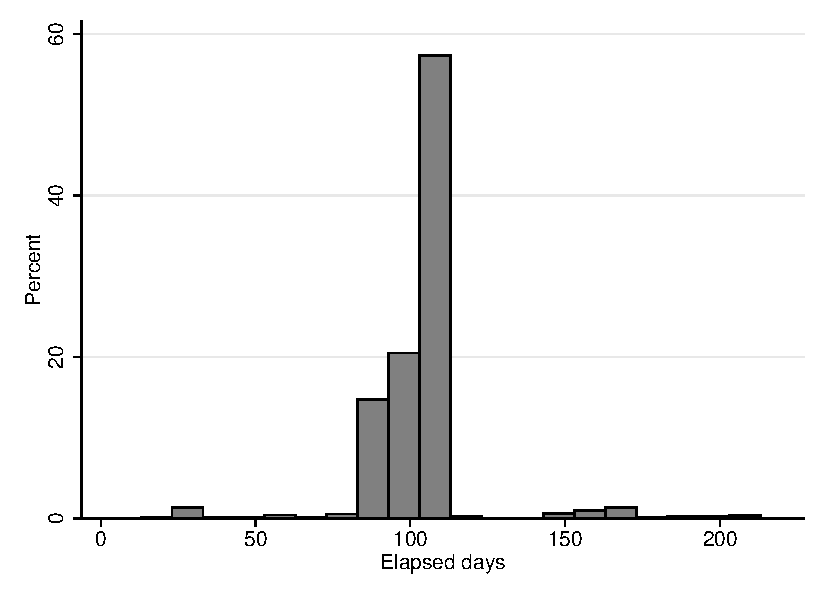
\includegraphics[width=\textwidth]{Figuras/hist_firstdays_default.pdf}
    \end{subfigure}
    \begin{subfigure}{0.40\textwidth}
        \caption{Elapsed days to last payment}
        \centering
        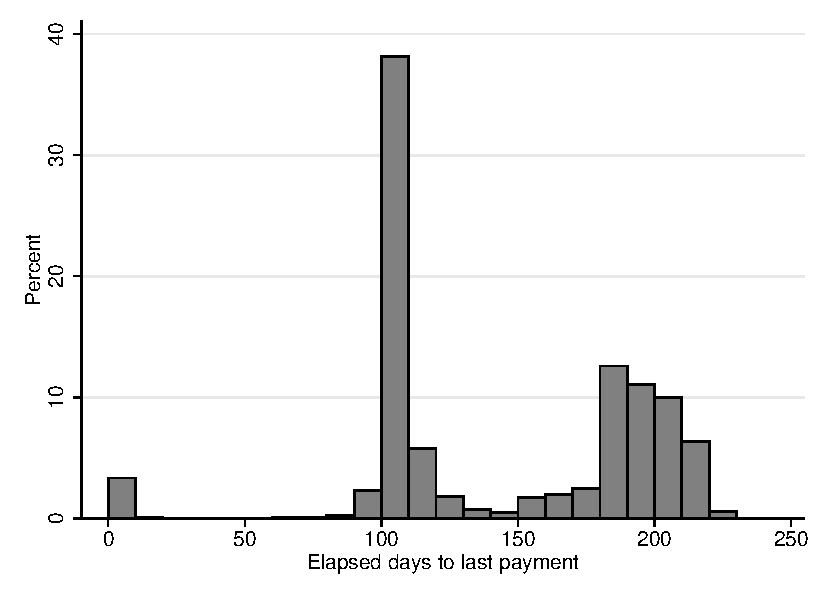
\includegraphics[width=\textwidth]{Figuras/hist_days_default.pdf}
    \end{subfigure}
        \begin{subfigure}{0.40\textwidth}
        \caption{Payments as \% of loan}
        \centering
        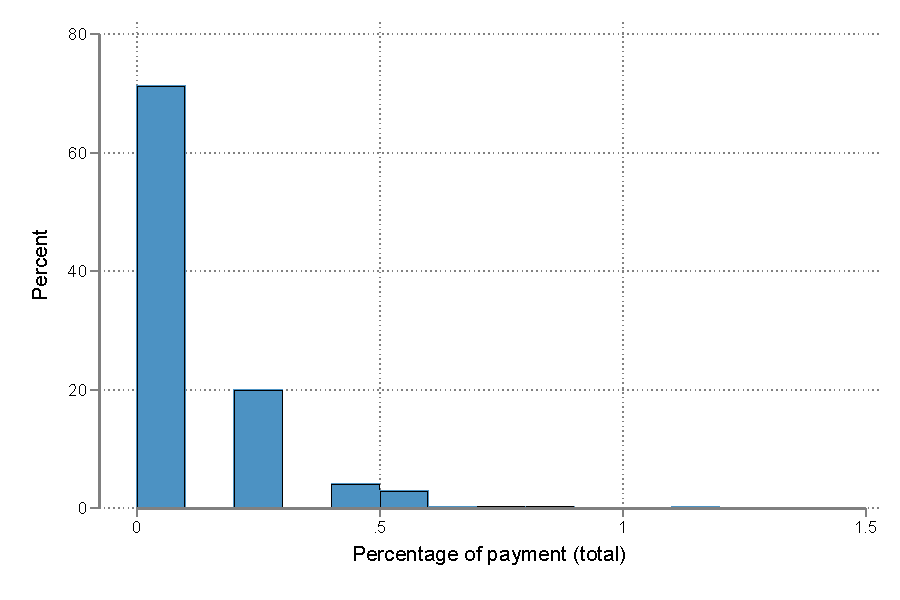
\includegraphics[width=\textwidth]{Figuras/hist_percpay_default.pdf}
    \end{subfigure}
    \begin{subfigure}{0.40\textwidth}
        \caption{Number of payments}
        \centering
        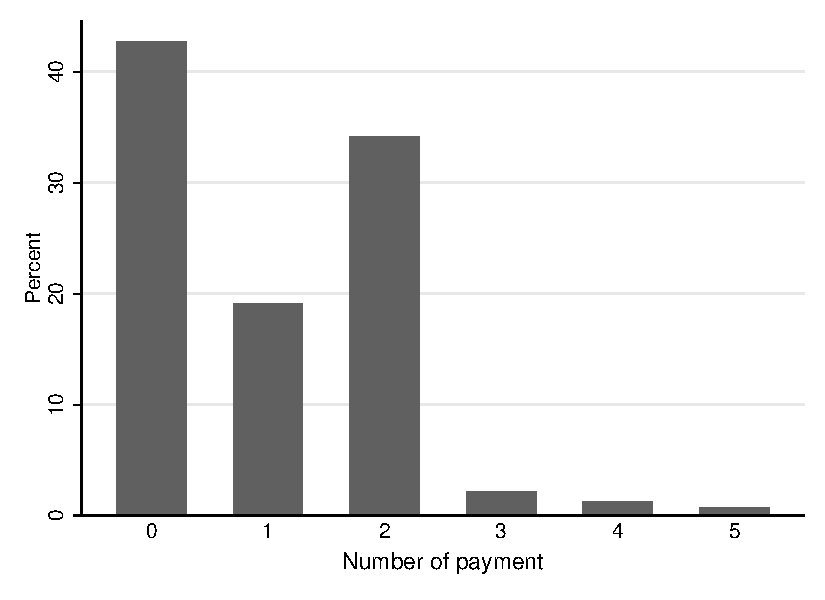
\includegraphics[width=\textwidth]{Figuras/hist_numpay_default.pdf}
    \end{subfigure}
    \end{center}
        \scriptsize 
        This figure describes behavior for the subsample of clients whose pawn was not recovered (in the control group).  Panel (a) shows days elapsed from the pawn to the first payment, while panel (b) displays the days elapsed to last payment. Some people pay after the day 105 when the grace period ends because the can ``restart'' the loan if they pay all interest owed. It amounts to starting a new loan with the same conditions and same pawn. Panel (c) shows the fraction of the loan that they paid (even when they ended up losing the pawn). Panel (d) displays the number of times they went to the branch to pay.      
      %\textit{Do file: }  \texttt{hist\_den\_default.do}
\end{figure}


\newpage
\subsection{Main treatment effects: Additional material}

\vspace{.2in}



\begin{figure}[H]
        \caption{FC conditional on first 115 days - treatment effect}
    \label{fc_pro_2_115}
    \begin{center}
        \centering
        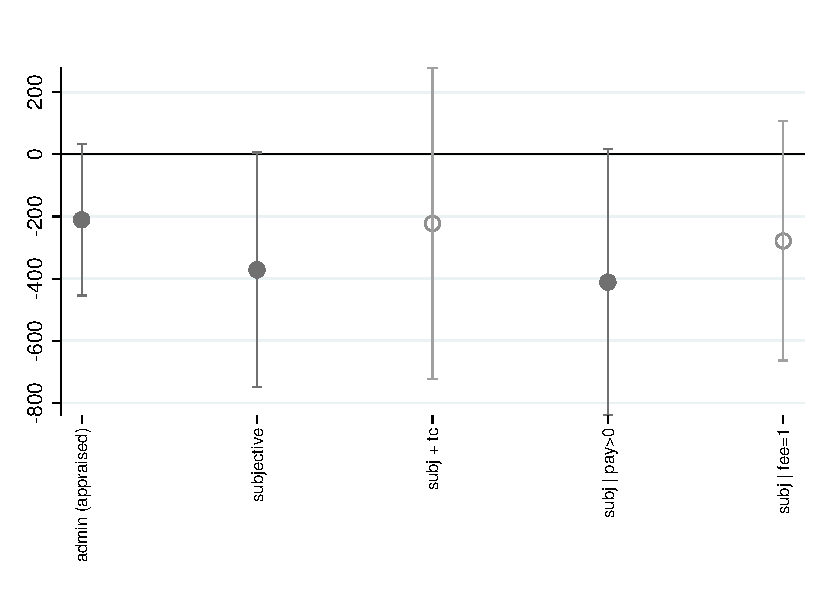
\includegraphics[width=0.50\textwidth]{Figuras/fc_te_115_pro_2.pdf}
    \end{center}
     \scriptsize This figure is the same as in Figure \ref{fc_pro2} Panel (a), but with the subsample restricted to the first 115 days.
     %\textit{Do file: }  \texttt{fc\_te\_115.do}
\end{figure}



\begin{figure}[H]
        \caption{Financial cost effect: charging all fees}
    \label{fc_allfee}
    \begin{center}
        \centering
        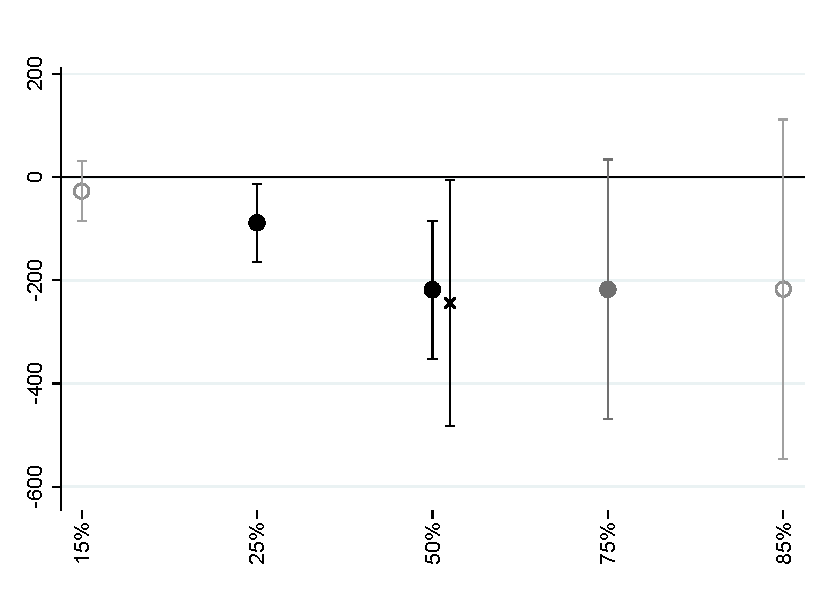
\includegraphics[width=0.50\textwidth]{Figuras/fc_allfee_quantile_pro_2.pdf}
    \end{center}
    \scriptsize
     This figure is the analogous to Figure \ref{fc_pro2}(b), except that for the fee-forcing contract we pretend that all clients incurred in their late fees, and therefore inflate the financial cost by summing those fees. This is intended as a kind of worse case scenario for the financial cost of the fee-forcing contract. The circles indicate the quantile treatment effects, while the cross is the (OLS) mean. We still find that the financial cost of will be smaller under the fee-forcing contract in spite of artificially inflating it.
     %\texttt{fc\_all\_fee.do}
\end{figure}





\begin{figure}[H]
        \caption{FC as \% of loan - treatment effect}
    \label{fc_perc}
    \begin{center}
        \centering
        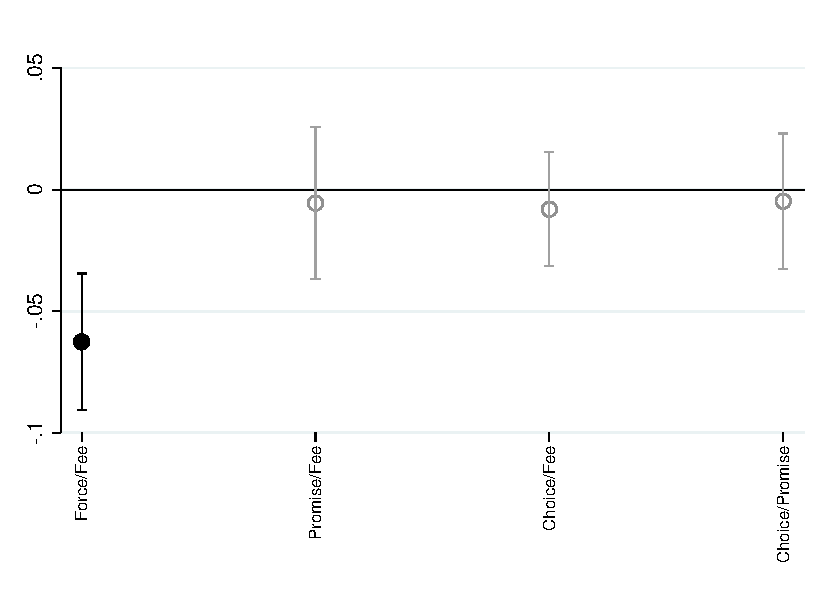
\includegraphics[width=0.50\textwidth]{Figuras/fc_perc_te_allarms.pdf}
    \end{center}
     \scriptsize This figure shows the estimated treatment effect of all arms against the status quo, but normalizing the dependent variable by the value of the loan.
     %\textit{Do file: }  \texttt{fc\_perc\_allarms.do}
\end{figure}




\begin{figure}[H]
    \caption{Relationship between treatment effects}
    \label{induced_to_pay_early}
    \begin{center}
    \begin{subfigure}{0.45\textwidth}
        \caption{\footnotesize{Induced to pay earlier vs Induced Lower FC}}
        \centering
        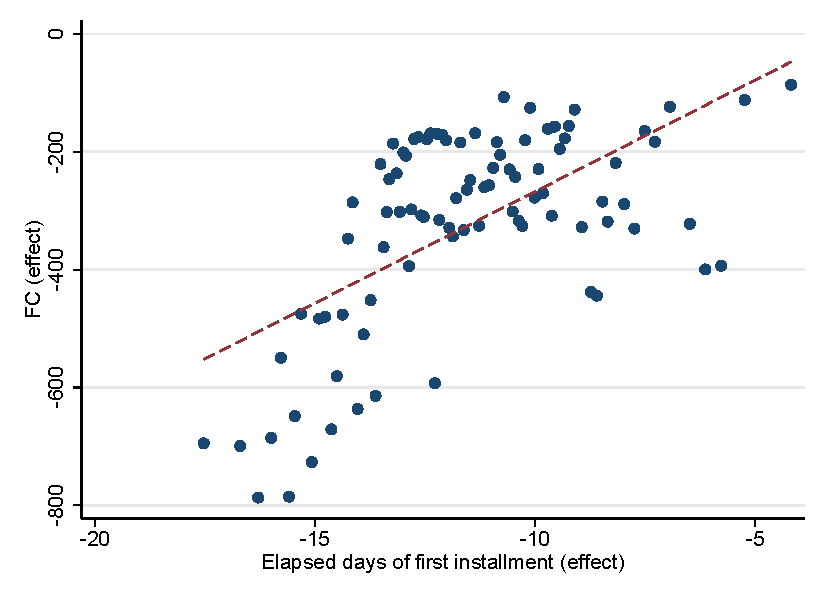
\includegraphics[width=\textwidth]{Figuras/binscatter_fc_days_pro_2.pdf}
    \end{subfigure}
        \begin{subfigure}{0.45\textwidth}
        \caption{\footnotesize{Induced to pay earlier vs Induced Recovery}}
        \centering
        \includegraphics[width=\textwidth]{Figuras/binscatter_def_days_pro_2.pdf}
    \end{subfigure}
    \end{center}
       \scriptsize 
       This figure plots relationships between \textit{treatment effects}. Both Panels (a) an (b) have the same X-axis, which displays the estimated heterogeneous treatment effect on the outcome ``elapsed days of first payment'', that is how many days elapsed from the day the loan was awarded to the first payment the client made. The treatments effects were calculated using \cite{atheygrf}. In Panel (a) the Y-axis is the \textit{treatment effect} on financial cost. In Panel (b) the Y-axis is the \textit{treatment effect} on losing their pawn. Panel (a) shows that those induced to pay earlier are also those that have larger savings in financial cost as a result of ``forcing'' the frequent payment commitment contract compared to the status-quo (control). Panel (b) shows that those induced to pay earlier are also those that have a larger increase in recovery.
      %\textit{Do file: }  \texttt{binscatter\_hte.do}
\end{figure}

\begin{figure}[H]
        \caption{Repeat purchase before 30/60 days}
    \label{reincidence_before}
    \begin{center}
        \centering
        \includegraphics[width=0.50\textwidth]{Figuras/re_te_earlydays.pdf}
    \end{center}
     \scriptsize This figure shows the estimated treatment effect of repeat purchase before 30 \& 60 days.
     %\textit{Do file: }  \texttt{re\_te\_earlydays.do}
\end{figure}


\newpage

\begin{table}[H]
\caption{Intermediate outcomes}
\label{mechanisms}
\begin{center}
\scriptsize{% Table generated by Excel2LaTeX from sheet 'mechanism'
\begin{tabular}{lccccccc}
\toprule
      & \% of payment in 1st visit & $\Pr($Recovery in 1st visit) & \% of payment & $\Pr($+ payment \& default) & \% of pay $|$ def  & $\Pr($Selling pawn) & $\Pr($Selling pawn $|$ def) \\
\midrule
\midrule
      & (1)   & (2)   & (3)   & (4)   & (5)   & (6)   & (7) \\
\midrule
\midrule
Forced commitment & 7.92*** & 0.079*** & 9.43*** & -0.070*** & -3.90*** & 0.0050 & 0.14*** \\
      & (2.78) & (0.026) & (2.62) & (0.015) & (1.26) & (0.021) & (0.034) \\
Choice commitment & -0.97 & -0.010 & 1.40  & -0.026* & -1.75* & 0.0035 & 0.049* \\
      & (2.20) & (0.022) & (2.36) & (0.013) & (1.00) & (0.019) & (0.029) \\
      &       &       &       &       &       &       &  \\
\midrule
Observations & 6304  & 6304  & 6304  & 6304  & 2488  & 6304  & 2488 \\
R-squared & 0.014 & 0.016 & 0.015 & 0.011 & 0.022 & 0.016 & 0.033 \\
Control Mean & 44.7  & 0.30  & 67.2  & 0.12  & 9.46  & 0.31  & 0.72 \\
\midrule
\midrule
      &       &       &       &       &       &       &  \\
\midrule
      & Days to 1st payment & \# of visits & \# of visits $|$ recovery & \# of visits $|$ def & Loan duration (days) & Loan duration $|$ recovery &  \\
\midrule
\midrule
      & (8)   & (9)   & (10)  & (11)  & (12)  & (13)  &  \\
\midrule
\midrule
Forced commitment & -13.8*** & -0.031 & -0.19*** & 0.062 & -27.9*** & -17.9*** &  \\
      & (1.61) & (0.049) & (0.049) & (0.053) & (4.35) & (3.88) &  \\
Choice commitment & -3.51** & 0.085 & -0.077* & 0.13** & -0.18 & -1.35 &  \\
      & (1.57) & (0.053) & (0.041) & (0.063) & (4.33) & (4.19) &  \\
      &       &       &       &       &       &       &  \\
\midrule
Observations & 4412  & 6304  & 2488  & 3031  & 6304  & 3031  &  \\
R-squared & 0.055 & 0.022 & 0.025 & 0.018 & 0.054 & 0.041 &  \\
Control Mean & 82.8  & 1.14  & 0.39  & 1.44  & 136.6 & 103.9 &  \\
\bottomrule
\bottomrule
\end{tabular}%
}
\end{center}

%\textit{Do file: } \texttt{mechanisms.do}
\end{table}

\scriptsize {
\noindent This table explores treatment effects in ``intermediate variables''. Each column represents a different dependent variable in an OLS regression, and each panel represents a different treatment arm-control comparison. All regressions include fixed effects for branch, day of week fixed effects, number of pawns at the time of pawning this particular one, number of different treatment arms experienced before pawning this particular one. $R^2$ are not reported, they were less than 0.04 for all but the last column which had $R^2$'s close to 0.6. The last row shows the mean of the dependent variable for the control group. Dependent variables are as follows: Column (1) measures the number of days elapsed from the pawning date to the first payment done. Column (2) records the number of payments done within 230 days of the pawn. Column (3) is the average size of the payments for each client in pesos. Column (4) is self-reported cost to get to the branch plus the imputed loss of a whole day of salary (using the minimum wage in Mexico) multiplied by the number of visits to the branch. Column (5) measures the number of days it took to recover the pawn, conditional on recovering. The dependent variable in Column (6) is a dummy =1 if the client paid any positive amount within 230 days of the pawn. For Columns (7) and (8) the dependent variable it is the sum of total payments done within 230 days of the pawn divided by the size of the loan, but column (8) includes as regressors a dummy=1 if the client recovered her pawn, and its interaction with treatment.
}

\vspace{3ex}

\vspace{.3in}

\subsection{FOSD: fee forcing vs status quo financial cost distributions}


\vspace{.2in}
\begin{figure}[H]
        \caption{Empirical CDF of Financial Cost: fee-focing vs status-quo}
    \label{ecdf_fc}
    \begin{center}
        \centering
        \includegraphics[width=0.65\textwidth]{Figuras/cdf_fc_pro_2.pdf}
    \end{center}
    \scriptsize This figure plots the empirical cumulative distribution of financial cost. It does this separately for the fee-forcing contract and for the status-quo contract. The doted line at the bottom is the difference of the status-quo CDF minus the fee-focing CDF. It shows that the CDF of the status quo contract is always below that of the fee-forcing (and this difference is significant for the points indicated by the blue line), and therefore that the former first-order stochastically dominates the later for weakly decreasing utility functions; see Proposition \ref{eq_fosd}.
    % \texttt{ecdf\_fc.do}}
\end{figure}



\vspace{.2in}
\begin{table}[H]
\caption{Clients who should prefer fee-forcing financial cost distribution}
\label{stochastic_dominance}
\begin{center}
\scriptsize{% Table generated by Excel2LaTeX from sheet 'dominance'
\begin{tabular}{lccc}
\toprule
Sub-population & Dominance & Log-normality (AD/KS) & Obs \\
\midrule
\midrule
Fee-forcing & \cellcolor[rgb]{ .557,  .663,  .859} $\succeq_{1}^*$ & */*  |  */* & 5034 \\
Low-loan & $\succeq_{1}^*$ &    /     |     /    & 2508 \\
High-loan & $\succeq_{1}^*$ &    /     |     /    & 2526 \\
Low-subj. prob. & \cellcolor[rgb]{ .557,  .663,  .859} $\succeq_{1}^*$ & */*  |  */* & 1083 \\
High-subj. Prob. & \cellcolor[rgb]{ .557,  .663,  .859} $\succeq_{1}^*$ & */*  |  */* & 2590 \\
Low-age & $\preceq_{1}$ & */*  |  */* & 1358 \\
High-age & \cellcolor[rgb]{ .851,  .882,  .949} $\succeq_{1}$ & */*  |     /* & 1362 \\
Low-income index & \cellcolor[rgb]{ .851,  .882,  .949} $\succeq_{1}$ & */*  |  */* & 1047 \\
High-income index & \cellcolor[rgb]{ .851,  .882,  .949} $\succeq_{1}$ & */*  |  */* & 948 \\
Male  & -     & */*  |     /* & 755 \\
Female & \cellcolor[rgb]{ .851,  .882,  .949} $\succeq_{1}$ & */*  |  */* & 2158 \\
First time & $\preceq_{1}$ & */*  |  */* & 293 \\
Pawn before & \cellcolor[rgb]{ .851,  .882,  .949} $\succeq_{1}$ & */*  |  */* & 2475 \\
Family doesn't ask & $\preceq_{1}$ & */*  |  */* & 1826 \\
Family asks & \cellcolor[rgb]{ .557,  .663,  .859} $\succeq_{1}^*$ & */*  |  */* & 987 \\
Not common ask & \cellcolor[rgb]{ .851,  .882,  .949} $\succeq_{1}$ & */*  |  */* & 1436 \\
Common asks & -     & */*  |  */* & 625 \\
No savings & $\preceq_{1}$ & */*  |  */* & 1353 \\
Has savings & \cellcolor[rgb]{ .557,  .663,  .859} $\succeq_{1}^*$ & */*  |  */* & 717 \\
Not rosca & \cellcolor[rgb]{ .557,  .663,  .859} $\succeq_{1}^*$ & */*  |  */* & 1270 \\
Rosca & $\preceq_{1}$ & */*  |  */* & 795 \\
Low-education & \cellcolor[rgb]{ .851,  .882,  .949} $\succeq_{1}$ & */*  |     /* & 906 \\
High-education & \cellcolor[rgb]{ .851,  .882,  .949} $\succeq_{1}$ & */*  |  */* & 1797 \\
Not stressed & -     & */*  |  */* & 1998 \\
Stressed & -     & */*  |  */* & 839 \\
Not overconfident & $\preceq_{1}$ & */*  |  */* & 47 \\
Overconfident & \cellcolor[rgb]{ .851,  .882,  .949} $\succeq_{1}$ & */*  |     /* & 1626 \\
Not PB & \cellcolor[rgb]{ .851,  .882,  .949} $\succeq_{1}$ & */*  |  */* & 1438 \\
PB    & \cellcolor[rgb]{ .557,  .663,  .859} $\succeq_{1}^*$ & */*  |     /* & 226 \\
Not FB & \cellcolor[rgb]{ .851,  .882,  .949} $\succeq_{1}$ & */*  |  */* & 1521 \\
FB    & \cellcolor[rgb]{ .851,  .882,  .949} $\succeq_{1}$ & */*  |  */* & 143 \\
Doesn't make budget & \cellcolor[rgb]{ .851,  .882,  .949} $\succeq_{1}$ & */*  |  */* & 1054 \\
Makes budget & \cellcolor[rgb]{ .851,  .882,  .949} $\succeq_{1}$ & */*  |  */* & 1689 \\
Not tempted & \cellcolor[rgb]{ .851,  .882,  .949} $\succeq_{1}$ & */*  |     /* & 875 \\
Tempted & \cellcolor[rgb]{ .851,  .882,  .949} $\succeq_{1}$ & */*  |  */* & 1872 \\
High-transp. cost & \cellcolor[rgb]{ .851,  .882,  .949} $\succeq_{1}$ & */*  |  */* & 1352 \\
Low-transp. cost & \cellcolor[rgb]{ .851,  .882,  .949} $\succeq_{1}$ & */*  |  */* & 1343 \\
High-transp. time & \cellcolor[rgb]{ .851,  .882,  .949} $\succeq_{1}$ & */*  |  */* & 1260 \\
Low-transp. time & \cellcolor[rgb]{ .557,  .663,  .859} $\succeq_{1}^*$ & */*  |  */* & 1442 \\
\bottomrule
\bottomrule
\end{tabular}%
}
\end{center}
 \scriptsize
This table does two things. First, it tests whether the observed empirical distribution of financial cost is well approximated by a log normal. It does this using two tests, the Anderson-Darling and the Kolmogorov-Smirnoff tests. Second, it fits a log normal distribution by maximum likelihood to observed empirical distribution of financial cost, separately for the fee-forcing arm and the status-quo arm. Using the fitted log normal, it tests whether the fee-forcing financial cost distribution would be preferred by any expected utility agent using Proposition \ref{lognormal_fosd} below. The different rows of the table do this for different sub-populations.  The first row of the table does it for every client in the fee forcing and status quo arms. The ``*'' show that we cannot reject at the 5\% level that both distribution are log normal for any of the two tests. The column entitled ``Dominance'' shows whether any client that dislikes higher cost would prefer the fee-forcing cost distribution over the status quo one, with $\succeq_{1}$ meaning he should (with $\succeq_{1}^*$ indicating the difference is statistically significant). It turns out to be the case that for the overwhelming majority of sub-populations, the conditions of preferring the fee-forcing distribution hold.
%\textit{Do file: } \texttt{stoch\_dominance.do}
\end{table}


\vspace{.2in}
\begin{prop}
\label{lognormal_fosd}
\footnotesize{
Let $F$ and $G$ be the cumulative distributions of two alternative log-normal prospects. The following are equivalent:

\begin{enumerate}[(a)]
    \item For every weakly decreasing utility function $u$: $E_{F}(u(FC))\leq E_G(u(FC))$
    \item $E_F \log(FC)\geq E_G\log(FC)$ and $Var_F \log(FC)= Var_G\log(FC)$
\end{enumerate}
}
\end{prop}

\begin{proof}
\footnotesize{
See Theorem 4 in \cite{lognormal_dominance}.
}
\end{proof}

\newpage

\vspace{.1in}
\begin{prop}
\label{eq_fosd}
\footnotesize{
This is a standard result. 
\\
\vspace{.1in}
The following are equivalent:
\begin{enumerate}[(a)]
    \item For every weakly decreasing utility function $u$: $E_{sq}(u(FC))\leq E_{fee}(u(FC))$
    \item $F_{sq}(FC)\leq F_{fee}(FC)$ 
\end{enumerate}
}
\end{prop}
\begin{proof} \;
\footnotesize{

[$(a)\Longrightarrow (b)$] Suppose  $(b)$ does not hold. So there exists $FC^*$ such that $F_{sq}(FC^*)>F_{fee}(FC^*)$, Define $u:=\mathds{1}_{FC\leq FC^*}$. Then
\[E_{sq}(u(FC)) = \int u(FC)dF_{sq} = F_{sq}(FC^*)>F_{fee}(FC^*)= \int u(FC)dF_{fee} =E_{fee}(u(FC))\]
which contradicts $(a)$.\\

[$(a)\Longleftarrow (b)$] On the other hand for $u$ weakly decreasing,

\[\int u(y(FC))dF_{sq}(y(FC)) = \int u(y(FC))dF_{fee}(FC) \leq \int u(FC)dF_{fee}(FC)\]
with $y(FC) = F_{sq}^{-1}F_{fee}(FC)$.
}
\end{proof}
\footnotesize{
Note the proof was done in the case of absolutely continuous and strictly increasing distribution functions $F_{sq}$ and $F_{fee}$.
}




\newpage
\subsection{Causal Random Forest and HTE}

\vspace{.3in}
\begin{figure}[H]
        \caption{Honest causal tree for the fee forcing contract heterogenous treatment effects}
    \label{casual_tree}
    \begin{center}
        \centering
        \includegraphics[width=.8\textwidth]{Figuras/crf_pro_2_fc_admin_disc.pdf}
    \end{center}
    \footnotesize 
    This is one(it is chosen such that it minimizes the pruned cost, that is it is the tree with the smallest root-node impurity) of the honest causal trees in the random forest we use for the estimation of the heterogeneous treatment effect of the fee-forcing contract. It is meant only as an example of how these trees look like. The forest was such that there are as many estimated treatment effects as there are clients.
     %\footnotesize{ \textit{RScript: }  \texttt{grf.R}
\end{figure}

We use \cite{atheygrf} \texttt{causal\_forest} of the \texttt{grf} library in $R$. The parameters used were:
\scriptsize{\textit{causal\_forest(
  X, 
  Y, 
  W, 
  Y.hat = NULL, 
  W.hat = NULL, 
  num.trees = 2000, 
  sample.weights = NULL, 
  clusters = NULL, 
  equalize.cluster.weights = FALSE, 
  sample.fraction = 0.5, 
  mtry = min(ceiling(sqrt(ncol(X)) + 20),ncol(X)), 
  min.node.size = 5, 
  honesty = TRUE, 
  honesty.fraction = 0.5, 
  honesty.prune.leaves = TRUE, 
  alpha = 0.05, 
  imbalance.penalty = 0, 
  stabilize.splits = TRUE, 
  ci.group.size = 2, 
  tune.parameters = "none", 
  tune.num.trees = 200, 
  tune.num.reps = 50, 
  tune.num.draws = 1000, 
  compute.oob.predictions = TRUE, 
  orthog.boosting = FALSE, 
  num.threads = NULL)}}



\begin{figure}[H]
    \caption{Heterogeneous Treatment Effect: Fee-forcing contract}
    \label{HTE_fee_forcing}
    \begin{center}
    %\begin{subfigure}{0.4\textwidth}
    %    \caption{Financial cost}
    %    \centering
    %    \includegraphics[width=\textwidth]{Figuras/he_dist_fc_admin_disc_pro_2.pdf}
    %\end{subfigure}
    \begin{subfigure}{0.7\textwidth}
        \caption{Determinants of effects}
        \centering
        \includegraphics[width=\textwidth]{Figuras/HE/he_int_vertical_fc_admin_disc_pro_2.pdf}
    \end{subfigure}
    
    %\begin{subfigure}{0.4\textwidth}
    %    \caption{Losing Pawn}
    %    \centering
    %    \includegraphics[width=\textwidth]{Figuras/he_dist_def_c_pro_2.pdf}
    %\end{subfigure}
    %\begin{subfigure}{0.4\textwidth}
    %    \caption*{}
    %    \centering
    %    \includegraphics[width=\textwidth]{Figuras/HE/he_int_vertical_def_c_pro_2.pdf}
    %\end{subfigure}
    \end{center}
     \scriptsize  This figure estimates bivariate regressions of the estimated client-level heterogeneous treatment effects against the respective covariate from the baseline survey  $\widehat{hte_i} = \alpha + \beta \: X_i + \epsilon_i$. The regressors $X_i$ include (e.g if the family asks for money, if they have savings, if they are overconfident using the definition the text, etc. See this Appendix for a transcription of the survey).
      %\footnotesize{ \textit{Do file: }  \texttt{analyze\_grf\_single\_arm.do}}
\end{figure}



\begin{comment}
\begin{figure}[H]
    \caption{Heterogeneous Treatment Effect: Promise-forcing contract}
    \label{heterogeneous_te_3}
    \begin{center}
    \begin{subfigure}{0.4\textwidth}
        \caption{Financial cost}
        \centering
        \includegraphics[width=\textwidth]{Figuras/he_dist_fc_admin_disc_pro_3.pdf}
    \end{subfigure}
    \begin{subfigure}{0.4\textwidth}
        \caption*{}
        \centering
        \includegraphics[width=\textwidth]{Figuras/HE/he_int_vertical_fc_admin_disc_pro_3.pdf}
    \end{subfigure}
    
    \begin{subfigure}{0.4\textwidth}
        \caption{Losing Pawn}
        \centering
        \includegraphics[width=\textwidth]{Figuras/he_dist_def_c_pro_3.pdf}
    \end{subfigure}
    \begin{subfigure}{0.4\textwidth}
        \caption*{}
        \centering
        \includegraphics[width=\textwidth]{Figuras/HE/he_int_vertical_def_c_pro_3.pdf}
    \end{subfigure}
    \end{center}
     \scriptsize
      %\footnotesize{ \textit{Do file: }  \texttt{analyze\_grf\_single\_arm.do}}
\end{figure}
\end{comment}





\begin{comment}

\begin{figure}[H]
    \caption{Heterogeneous Treatment Effect - Choice/Fee}
    \label{heterogeneous_te_4}
    \begin{center}
    \begin{subfigure}{0.4\textwidth}
        \caption{Financial cost}
        \centering
        \includegraphics[width=\textwidth]{Figuras/he_dist_fc_admin_disc_pro_4.pdf}
    \end{subfigure}
    \begin{subfigure}{0.4\textwidth}
        \caption*{}
        \centering
        \includegraphics[width=\textwidth]{Figuras/HE/he_int_vertical_fc_admin_disc_pro_4.pdf}
    \end{subfigure}
    
    \begin{subfigure}{0.4\textwidth}
        \caption{Losing Pawn}
        \centering
        \includegraphics[width=\textwidth]{Figuras/he_dist_def_c_pro_4.pdf}
    \end{subfigure}
    \begin{subfigure}{0.4\textwidth}
        \caption*{}
        \centering
        \includegraphics[width=\textwidth]{Figuras/HE/he_int_vertical_def_c_pro_4.pdf}
    \end{subfigure}
    \end{center}
     \footnotesize \textit{Notes: } The distribution plots the FC treatment effect for the interval $[\mu-2\sigma,\mu+2\sigma]$ to ignore the outliers.
      \footnotesize{ \textit{Do file: }  \texttt{analyze\_grf\_single\_arm.do}}
\end{figure}




\begin{figure}[H]
    \caption{Heterogeneous Treatment Effect - Choice/Promise}
    \label{heterogeneous_te_5}
    \begin{center}
    \begin{subfigure}{0.4\textwidth}
        \caption{Financial cost}
        \centering
        \includegraphics[width=\textwidth]{Figuras/he_dist_fc_admin_disc_pro_5.pdf}
    \end{subfigure}
    \begin{subfigure}{0.4\textwidth}
        \caption*{}
        \centering
        \includegraphics[width=\textwidth]{Figuras/HE/he_int_vertical_fc_admin_disc_pro_5.pdf}
    \end{subfigure}
    \begin{subfigure}{0.4\textwidth}
        \caption{Losing Pawn}
        \centering
        \includegraphics[width=\textwidth]{Figuras/he_dist_def_c_pro_5.pdf}
    \end{subfigure}
    \begin{subfigure}{0.4\textwidth}
        \caption*{}
        \centering
        \includegraphics[width=\textwidth]{Figuras/HE/he_int_vertical_def_c_pro_5.pdf}
    \end{subfigure}
    \end{center}
     \footnotesize \textit{Notes: } 
      \footnotesize{ \textit{Do file: }  \texttt{analyze\_grf\_single\_arm.do}}
\end{figure}

\end{comment}







%\begin{figure}[H]
%    \caption{Heterogeneous Treatment Effect (FC survey) - All arms}
%    \label{heterogeneous_te_fcsurvey_all}
%    \begin{center}
%    \begin{subfigure}{0.4\textwidth}
%        \caption{Forcing/Fee}
%        \centering
%        \includegraphics[width=\textwidth]{Figuras/he_dist_fc_survey_disc_pro_2.pdf}
%    \end{subfigure}
%    \begin{subfigure}{0.4\textwidth}
%        \caption{Forcing/Promise}
%        \centering
%        \includegraphics[width=\textwidth]{Figuras/he_dist_fc_survey_disc_pro_3.pdf}
%    \end{subfigure}
    
%    \begin{subfigure}{0.4\textwidth}
%        \caption{Choice/Fee}
%        \centering
%        \includegraphics[width=\textwidth]{Figuras/he_dist_fc_survey_disc_pro_4.pdf}
%    \end{subfigure}
%    \begin{subfigure}{0.4\textwidth}
%        \caption{Choice/Promise}
%        \centering
%        \includegraphics[width=\textwidth]{Figuras/he_dist_fc_survey_disc_pro_5.pdf}
%    \end{subfigure}
%    \end{center}
%     \footnotesize \textit{Notes: } 
%      \footnotesize{ \textit{Do file: }  \texttt{analyze\_grf\_single\_arm.do}}
%\end{figure}



\subsection{Take up}


\begin{table}[H]
    \caption{Predicting Take-up: Goodness-of-Fit}
    \label{Table_compliance}
    %\begin{subtable}{1\textwidth}
    % \centering
    %    \caption{Take up}
    %    \scriptsize{% Table generated by Excel2LaTeX from sheet 'oos_pago_frec_vol'
\begin{tabular}{lcccc}
\toprule
      & \multicolumn{4}{c}{Frequent voluntary payment } \\
\midrule
\midrule
OOS measures & Logit & SW-Logit & RF    & Boosting \\
\midrule
\midrule
MAE   & 0.32  & 0.33  & 0.33  & 0.29 \\
MSE   & 0.17  & 0.17  & 0.16  & 0.16 \\
AUC (out of sample) & 0.71  & 0.71  & 0.77  & 0.73 \\
      & (0.04) & (0.04) & (0.04) & (0.04) \\
AUC (in sample) & 0.77  & 0.76  & 0.88  & 0.96 \\
      & (0.02) & (0.02) & (0.01) & (0.01) \\
Accuracy & 0.7   & 0.7   & 0.75  & 0.77 \\
Correlation (0-1) & 0.21  & 0.22  & 0.39  & 0.38 \\
Correlation (predicted val) & 0.33  & 0.33  & 0.42  & 0.4 \\
R-squared  & 0.11  & 0.11  & 0.16  & 0.15 \\
Expected value of predictions & 0.25  & 0.25  & 0.24  & 0.22 \\
\bottomrule
\bottomrule
\end{tabular}%
}
    %\end{subtable}%
    
    %\bigskip
     \begin{subtable}{1\textwidth}
      \centering
        \caption{Take up: Choice-fee Arm}
        \scriptsize{% Table generated by Excel2LaTeX from sheet 'oos_pago_frec_vol_fee'
\begin{tabular}{lcccc}
\toprule
      & \multicolumn{4}{c}{Frequent voluntary payment - FEE} \\
\midrule
\midrule
OOS measures & Logit & SW-Logit & RF    & Boosting \\
\midrule
\midrule
MAE   & 0.21  & 0.21  & 0.23  & 0.17 \\
MSE   & 0.1   & 0.1   & 0.1   & 0.09 \\
AUC (out of sample) & 0.76  & 0.78  & 0.84  & 0.85 \\
      & (0.06) & (0.06) & (0.06) & (0.05) \\
AUC (in sample) & 0.84  & 0.82  & 0.92  & 0.99 \\
      & (0.02) & (0.02) & (0.01) & (0.01) \\
Accuracy & 0.82  & 0.84  & 0.86  & 0.88 \\
Correlation (0-1) & 0.13  & 0.26  & 0.37  & 0.31 \\
Correlation (predicted val) & 0.33  & 0.38  & 0.37  & 0.43 \\
R-squared  & 0.08  & 0.13  & 0.11  & 0.19 \\
Expected value of predictions & 0.17  & 0.17  & 0.16  & 0.12 \\
\bottomrule
\bottomrule
\end{tabular}%
}
    \end{subtable}
    
      \bigskip
    \begin{subtable}{1\textwidth}
      \centering
        \caption{Take up: Choice-promise Arm}
        \scriptsize{% Table generated by Excel2LaTeX from sheet 'oos_pago_frec_vol_promise'
\begin{tabular}{lcccc}
\toprule
      & \multicolumn{4}{c}{Frequent voluntary payment - PROMISE} \\
\midrule
\midrule
OOS measures & Logit & SW-Logit & RF    & Boosting \\
\midrule
\midrule
MAE   & 0.41  & 0.41  & 0.41  & 0.36 \\
MSE   & 0.24  & 0.23  & 0.21  & 0.21 \\
AUC (out of sample) & 0.63  & 0.63  & 0.7   & 0.72 \\
      & (0.06) & (0.06) & (0.06) & (0.06) \\
AUC (in sample) & 0.83  & 0.82  & 0.9   & 0.97 \\
      & (0.02) & (0.02) & (0.01) & (0.01) \\
Accuracy & 0.62  & 0.67  & 0.65  & 0.7 \\
Correlation (0-1) & 0.15  & 0.25  & 0.23  & 0.32 \\
Correlation (predicted val) & 0.22  & 0.21  & 0.3   & 0.35 \\
R-squared  & -0.06 & -0.05 & 0.08  & 0.08 \\
Expected value of predictions & 0.39  & 0.38  & 0.38  & 0.35 \\
\bottomrule
\bottomrule
\end{tabular}%
}
    \end{subtable}
            \scriptsize
           \\
           \\
           \\
    
     %\textit{Scripts: } \texttt{pred\_take\_up.do, pfv\_pred.R}
\end{table}




\vspace{.1in}
\begin{figure}[H]
    \caption{Out of sample ROC curve}
    \label{roc_curve}
    \begin{center}
    \begin{subfigure}{0.45\textwidth}
        \caption{Take-up in Fee Arm}
        \centering
        \includegraphics[width=\textwidth]{Figuras/Boost/ROC_curve_outsample_pago_frec_vol_fee.pdf}
    \end{subfigure}
    \begin{subfigure}{0.45\textwidth}
        \caption{Take-up in Promise Arm}
        \centering
        \includegraphics[width=\textwidth]{Figuras/Boost/ROC_curve_outsample_pago_frec_vol_promise.pdf}
    \end{subfigure}
    \end{center}
     \scriptsize 
  %\footnotesize{ \textit{Do file: }  \texttt{pred\_take\_up.do}}
\end{figure}



\begin{figure}[H]
    \caption{Predictors of commitment contract take-up}
    \label{interactions_takeup}
    \begin{center}
    \begin{subfigure}{0.45\textwidth}
        \caption{with Fee Arm}
        \centering
        \includegraphics[width=\textwidth]{Figuras/pago_frec_vol_fee_interactions_rf.pdf}
    \end{subfigure}
    \begin{subfigure}{0.45\textwidth}
        \caption{with Promise Arm}
        \centering
        \includegraphics[width=\textwidth]{Figuras/pago_frec_vol_promise_interactions_rf.pdf}
    \end{subfigure}
    \end{center}
     \scriptsize
      %\footnotesize{ \textit{Do file: }  \texttt{analyze\_fvp.do}}
\end{figure}


\scriptsize {
\noindent This figure reports bivariate regressions of the form $\widehat{TakeUp} = \alpha + \beta \: X_i + \epsilon_i$, where $\widehat{TakeUp}$ is the prediction using random forests. The figure reports the $\beta$ coefficients for different $X_i$'s along with 95\% confidence intervals. Panel (a) focuses on take up in the arm where clients could chose among the fee-commitment contract and the status quo contract. Panel (b) focuses on the arm where clients could chose among the promise-commitment contract and the status quo contract. Using random forests we can predict who takes up the fee-forcing contract with 85\% accuracy out of sample.\footnote{Correcting for the fact that most chose the status-quo contract using the method of SMOTE, \cite{smote} we find an accuracy rate of 75\%.} Which suggests that choice among contracts is not purely random. This figure shows that the more educated, those that report that their family typically asks for money, those that make a monthly budget of expenses, and those that ask for a remainder of their due payments (and marginally those we classify as present-biased) are more likely to chose the fee-commitment contract if given the choice. The opposite holds for clients that are more economically vulnerable (can barely pay for food, electricity, etc) and those that report being more stressed.
}


%---------------------------------------------------------------------------------------------------------------------------------------------------------------------------------------------------------------------------------

\newpage 

\subsection{New results}


\begin{table}[H]
\caption{Summary statistics and Balance}
\label{SS}
\begin{center}
\scriptsize{% Table generated by Excel2LaTeX from sheet 'SS_appendix'
\begin{tabular}{lcccccccc}
\toprule
      &       &       & \multicolumn{5}{c}{Treatment arms}    &  \\
\midrule
      &       &       &       & \multicolumn{2}{c}{No Choice } & \multicolumn{2}{c}{Choice} &  \\
\midrule
\midrule
      & Overall & Pre-experiment & Control & Fee   & Promise & Fee   & Promise & p-value \\
\midrule
      & \multicolumn{8}{c}{Panel A : Survey Data (conditional on pawning)} \\
\midrule
\midrule
Woman & 0.73  &       & 0.76  & 0.72  & 0.73  & 0.72  & 0.74  & 0.41 \\
      & (0.01) &       & (0.02) & (0.02) & (0.02) & (0.02) & (0.01) &  \\
Age   & 43.31 &       & 43.16 & 43.17 & 42.96 & 43.96 & 43.06 & 0.79 \\
      & (0.28) &       & (0.57) & (0.79) & (0.65) & (0.61) & (0.52) &  \\
Subjective value & 3069  &       & 3152  & 2978  & 2987  & 3115  & 3079  & 0.41 \\
      & (39)  &       & (69)  & (91)  & (76)  & (85)  & (100) &  \\
Has pawn before & 0.9   &       & 0.89  & 0.9   & 0.89  & 0.91  & 0.89  & 0.68 \\
      & (0)   &       & (0.01) & (0.01) & (0.01) & (0.01) & (0.01) &  \\
Subj. pr. of recovery & 93.14 &       & 92.74 & 92.16 & 93.6  & 93.67 & 93.3  & 0.45 \\
      & (0)   &       & (0.55) & (0.86) & (0.6) & (0.47) & (0.6) &  \\
+High-school & 0.66  &       & 0.66  & 0.67  & 0.65  & 0.67  & 0.64  & 0.73 \\
      & (0.01) &       & (0.02) & (0.02) & (0.02) & (0.02) & (0.02) &  \\
Survey response rate & 0.78  &       & 0.77  & 0.75  & 0.8   & 0.77  & 0.79  & 0.5 \\
      & (0.01) &       & (0.02) & (0.03) & (0.02) & (0.02) & (0.02) &  \\
\midrule
Obs   & 10432 &       & 2000  & 1855  & 1733  & 2652  & 2192  &  \\
\bottomrule
\bottomrule
\end{tabular}%
}
\end{center}
 \scriptsize

%\textit{Do file: } \texttt{SS\_appendix.do}
\end{table}


\begin{figure}[H]
        \caption{Financial cost for different discount rates}
    \label{fc_discount_rates}
    \begin{center}
        \centering
        \includegraphics[width=0.55\textwidth]{Figuras/discount_effect.pdf}
    \end{center}
     \scriptsize This Figure estimates the treatment effect on financial cost with different discount rates.  
     %\textit{Do file: }  \texttt{discounted\_noeffect.do}
\end{figure}



\begin{figure}[H]
    \caption{Treatment effects pooling all arms}
    \label{pooled_arms_te}
    \begin{center}
    \begin{subfigure}{0.45\textwidth}
        \caption{Financial Cost}
        \centering
        \includegraphics[width=\textwidth]{Figuras/te_allarms_fc_admin_disc.pdf}
    \end{subfigure}
    \begin{subfigure}{0.45\textwidth}
        \caption{Lost Pawn}
        \centering
        \includegraphics[width=\textwidth]{Figuras/te_allarms_def_c.pdf}
    \end{subfigure}
    \end{center}
     \scriptsize
      %\footnotesize{ \textit{Do file: }  \texttt{te\_allarms.do}}
\end{figure}


\scriptsize {
\noindent This Figure shows the treatment effects for the main outcomes when pooling all arms in the same regression.
}

\begin{figure}[H]
        \caption{Treatment effect decomposition of the Financial Cost }
    \label{reg_int_pro_2}
    \begin{center}
        \centering
        \includegraphics[width=0.60\textwidth]{Figuras/int_te_pro_2.pdf}
    \end{center}
     \scriptsize This Figure is a "close-up" for the estimates found in Figure \ref{fc_pro2} - Panel (a). It shows the treatment effects on payed \& incurred interest, the former defined as the actual interest payed, and the latter is the sum of all potential interests (for those pawns that were lost we calculate the interest generated until day 230). In the right axis we show the treatment effect on the payed fees. Finally, we analyze this effect for the subsamples that recovers or loses the pawn.
     %\textit{Do file: }  \texttt{reg_\int.do}
\end{figure}


\begin{figure}[H]
        \caption{Frequency of renewals}
    \label{ref_dist}
    \begin{center}
        \centering
        \includegraphics[width=0.60\textwidth]{Figuras/ref_dist.pdf}
    \end{center}
     \scriptsize  This Figure shows the occurrence and frequency of renewals. It locates in time, respective to the day the loan started, when the renewal occurs for both the first and second renewal. Note that the first renewal is concentrated around 100 days, while the second is concentrated around the 200 days, corresponding to the first and second cycle. 
     %\textit{Do file: }  \texttt{ref_\dist.do}
\end{figure}



\begin{figure}[H]
        \caption{Probability of recovery by arm}
    \label{survival_graph}
    \begin{center}
        \centering
        \includegraphics[width=0.60\textwidth]{Figuras/survival_graph_unpledge.pdf}
    \end{center}
     \scriptsize  This Figure shows the accumulated percentage of recovery in time by treatment arm. 
     %\textit{Do file: }  \texttt{survival\_graph.do}
\end{figure}





%\begin{figure}[H]
%    \caption{Exit Survey: reasons to pawn or not again with monthly payments}
%    \label{reasons}
%    \begin{center}
%    \begin{subfigure}{0.5\textwidth}
%        \caption{Pawn again because:}
%        \centering
%        \includegraphics[width=\textwidth]{Figuras/razones_si.pdf}
%    \end{subfigure}
%    \begin{subfigure}{0.5\textwidth}
%        \caption{Not pawn because:}
%        \centering
%        \includegraphics[width=\textwidth]{Figuras/razones_no.pdf}
%    \end{subfigure}
%    \end{center}
%     \footnotesize \textit{Notes: } 
%      \footnotesize{ \textit{Do file: }  \texttt{ss.do}}
%\end{figure}





%\begin{figure}[H]
%    \caption{Decomposition of the mistakes by `Overconfidence' for Promise Arms}
%    \label{Promise_errors}
%    \begin{center}
%    \begin{subfigure}{0.6\textwidth}
%        \caption{Promise}
%        \centering
%        \includegraphics[width=\textwidth]{Figuras/line_cw_fc_te_cf_OC_promise.pdf}
%    \end{subfigure}
%    \end{center}
%     \footnotesize 
%     \textit{Notes: }  Decomposition of the percentage of mistakes by overconfidence. 
%       \textit{Do file: }  \texttt{choose\_wrong\_quant\_wrong\_decomposition.do}
%\end{figure}




\begin{comment}
\begin{figure}[H]
        \caption{Histogram of payments}
    \label{HistPayments}
    \begin{center}
    \begin{subfigure}{.31\textwidth}
    \caption{Control}
        \centering
        \includegraphics[width=\textwidth]{Figuras/hist_payments_pro_1.pdf}
    \end{subfigure}
    \begin{subfigure}{.31\textwidth}
    \caption{Forcing - fee}
        \centering
        \includegraphics[width=\textwidth]{Figuras/hist_payments_pro_2.pdf}
    \end{subfigure}   
     \begin{subfigure}{.31\textwidth}
    \caption{Forcing - promise}
        \centering
        \includegraphics[width=\textwidth]{Figuras/hist_payments_pro_3.pdf}
    \end{subfigure}  
     \begin{subfigure}{.31\textwidth}
    \caption{Choice - fee}
        \centering
        \includegraphics[width=\textwidth]{Figuras/hist_payments_pro_4.pdf}
    \end{subfigure}  
     \begin{subfigure}{.31\textwidth}
    \caption{Choice - fee - SQ}
        \centering
        \includegraphics[width=\textwidth]{Figuras/hist_payments_pro_6.pdf}
    \end{subfigure}    
     \begin{subfigure}{.31\textwidth}
    \caption{Choice - fee - NSQ}
        \centering
        \includegraphics[width=\textwidth]{Figuras/hist_payments_pro_7.pdf}
    \end{subfigure}    
     \begin{subfigure}{.31\textwidth}
    \caption{Choice - promise}
        \centering
        \includegraphics[width=\textwidth]{Figuras/hist_payments_pro_5.pdf}
    \end{subfigure}  
     \begin{subfigure}{.31\textwidth}
    \caption{Choice - promise - SQ}
        \centering
        \includegraphics[width=\textwidth]{Figuras/hist_payments_pro_8.pdf}
    \end{subfigure}    
     \begin{subfigure}{.31\textwidth}
    \caption{Choice - promise - NSQ}
        \centering
        \includegraphics[width=\textwidth]{Figuras/hist_payments_pro_9.pdf}    
    \end{subfigure}        
    \end{center}
     \footnotesize \textit{Notes: } The x-axis shows the elapsed days between initial date and current movement.
      \footnotesize{ \textit{Do file: }  \texttt{hist\_payments.do}}
\end{figure}
\end{comment}

%\begin{figure}[H]
%        \caption{Types of agents that incur in different FC}
%    \label{components_fc}
%    \begin{center}
%        \centering
%        \includegraphics[width=\textwidth]{Figuras/scatter_fc_pay.pdf}
%    \end{center}
%     \footnotesize \textit{Notes: } 
%      \footnotesize{ \textit{Do file: }  \texttt{hist\_fc.do}}
%\end{figure}



\begin{comment}
\begin{figure}[H]
        \caption{Percentage of payments}
    \label{perc_payments}
    \begin{center}
    \begin{subfigure}{.31\textwidth}
    \caption{Control}
        \centering
        \includegraphics[width=\textwidth]{Figuras/hist_porc_pay_pro_1.pdf}
    \end{subfigure}
    \begin{subfigure}{.31\textwidth}
    \caption{Forcing - fee}
        \centering
        \includegraphics[width=\textwidth]{Figuras/hist_porc_pay_pro_2.pdf}
    \end{subfigure}   
     \begin{subfigure}{.31\textwidth}
    \caption{Forcing - promise}
        \centering
        \includegraphics[width=\textwidth]{Figuras/hist_porc_pay_pro_3.pdf}
    \end{subfigure}  
     \begin{subfigure}{.31\textwidth}
    \caption{Choice - fee}
        \centering
        \includegraphics[width=\textwidth]{Figuras/hist_porc_pay_pro_4.pdf}
    \end{subfigure}  
     \begin{subfigure}{.31\textwidth}
    \caption{Choice - fee - SQ}
        \centering
        \includegraphics[width=\textwidth]{Figuras/hist_porc_pay_pro_6.pdf}
    \end{subfigure}    
     \begin{subfigure}{.31\textwidth}
    \caption{Choice - fee - NSQ}
        \centering
        \includegraphics[width=\textwidth]{Figuras/hist_porc_pay_pro_7.pdf}
    \end{subfigure}    
     \begin{subfigure}{.31\textwidth}
    \caption{Choice - promise}
        \centering
        \includegraphics[width=\textwidth]{Figuras/hist_porc_pay_pro_5.pdf}
    \end{subfigure}  
     \begin{subfigure}{.31\textwidth}
    \caption{Choice - promise - SQ}
        \centering
        \includegraphics[width=\textwidth]{Figuras/hist_porc_pay_pro_8.pdf}
    \end{subfigure}    
     \begin{subfigure}{.31\textwidth}
    \caption{Choice - promise - NSQ}
        \centering
        \includegraphics[width=\textwidth]{Figuras/hist_porc_pay_pro_9.pdf}    
    \end{subfigure}        
    \end{center}
     \footnotesize \textit{Notes: } 
      \footnotesize{ \textit{Do file: }  \texttt{hist\_payments.do}}
\end{figure}




\begin{figure}[H]
        \caption{Percentage of payment conditional on positive payment and Losing Pawn}
    \label{perc_payments_conditional}
    \begin{center}
    \begin{subfigure}{.31\textwidth}
    \caption{Control}
        \centering
        \includegraphics[width=\textwidth]{Figuras/hist_porc_pay_cond_pro_1.pdf}
    \end{subfigure}
    \begin{subfigure}{.31\textwidth}
    \caption{Forcing - fee}
        \centering
        \includegraphics[width=\textwidth]{Figuras/hist_porc_pay_cond_pro_2.pdf}
    \end{subfigure}   
     \begin{subfigure}{.31\textwidth}
    \caption{Forcing - promise}
        \centering
        \includegraphics[width=\textwidth]{Figuras/hist_porc_pay_cond_pro_3.pdf}
    \end{subfigure}  
     \begin{subfigure}{.31\textwidth}
    \caption{Choice - fee}
        \centering
        \includegraphics[width=\textwidth]{Figuras/hist_porc_pay_cond_pro_4.pdf}
    \end{subfigure}  
     \begin{subfigure}{.31\textwidth}
    \caption{Choice - fee - SQ}
        \centering
        \includegraphics[width=\textwidth]{Figuras/hist_porc_pay_cond_pro_6.pdf}
    \end{subfigure}    
     \begin{subfigure}{.31\textwidth}
    \caption{Choice - fee - NSQ}
        \centering
        \includegraphics[width=\textwidth]{Figuras/hist_porc_pay_cond_pro_7.pdf}
    \end{subfigure}    
     \begin{subfigure}{.31\textwidth}
    \caption{Choice - promise}
        \centering
        \includegraphics[width=\textwidth]{Figuras/hist_porc_pay_cond_pro_5.pdf}
    \end{subfigure}  
     \begin{subfigure}{.31\textwidth}
    \caption{Choice - promise - SQ}
        \centering
        \includegraphics[width=\textwidth]{Figuras/hist_porc_pay_cond_pro_8.pdf}
    \end{subfigure}    
     \begin{subfigure}{.31\textwidth}
    \caption{Choice - promise - NSQ}
        \centering
        \includegraphics[width=\textwidth]{Figuras/hist_porc_pay_cond_pro_9.pdf}    
    \end{subfigure}        
    \end{center}
     \footnotesize \textit{Notes: } 
      \footnotesize{ \textit{Do file: }  \texttt{hist\_payments.do}}
\end{figure}
\end{comment}


%\begin{figure}[H]
%    \caption{Evolution of payment}
%    \label{Evolution payment}
%    \begin{center}
%    \begin{subfigure}{0.49\textwidth}
%        \caption{Paid loans}
%        \centering
%        \includegraphics[width=\textwidth]{Figuras/desempeno_evol.pdf}
%    \end{subfigure}
%     \begin{subfigure}{0.49\textwidth}
%      \caption*{}
%        \centering
%        \includegraphics[width=\textwidth]{Figuras/desempeno_evol_choice.pdf}
%    \end{subfigure}
    
%     \begin{subfigure}{0.49\textwidth}
%        \caption{Average percentage of paid loans}
%        \centering
%        \includegraphics[width=\textwidth]{Figuras/sum_porc_evol.pdf}
%    \end{subfigure}
%     \begin{subfigure}{0.49\textwidth}
%      \caption*{}
%        \centering
%        \includegraphics[width=\textwidth]{Figuras/sum_porc_evol_choice.pdf}
%    \end{subfigure}
    
%   \begin{subfigure}{0.49\textwidth}
%        \caption{Average percentage of paid loans | paid}
%        \centering
%        \includegraphics[width=\textwidth]{Figuras/sum_porc_cond_evol.pdf}
%    \end{subfigure}
%     \begin{subfigure}{0.49\textwidth}
%      \caption*{}
%        \centering
%        \includegraphics[width=\textwidth]{Figuras/sum_porc_cond_evol_choice.pdf}
%    \end{subfigure}
%    \end{center}
%     \footnotesize \textit{Notes: } 
%      \footnotesize{ \textit{Do file: }  \texttt{evol\_payment.do}}
%\end{figure}





\begin{comment}

\begin{figure}[H]
        \caption{FC effect for different discount rates}
    \label{oc_hist}
    \begin{center}
        \centering
        \includegraphics[width=0.50\textwidth]{Figuras/discount_effect.pdf}
    \end{center}
    \footnotesize \textit{Notes: } 
     \footnotesize{ \textit{Do file: }  \texttt{discounted\_noeffect.do}}
\end{figure}
\end{comment}

%%%%%%%%%%%%%%%%%%%%%%%%%%%%%%%%%%%%%%%%%%%%%%%
%%%%%%%%%%%%%%%%%%%%%%%%%%%%%%%%%%%%%%%%%%%%%%


% APPENDIX B

\newpage
\section{ Observational analysis}
\label{appendix_b}
\vspace{.2in}
\normalsize
\linespread{1.25}
%Really force it to normal size and linespread
\normalsize
\linespread{1.25}


The objective of this Appendix is to conduct one test aiming to assess if there is learning in choosing the frequent payment FP) contract. In particular if being endogenously induced to have a FP contract causes the client to chose a FP in subsequent pawn. The identification strategy is not as strong as in a randomized control trial ---having to rely on an instrumental variable strategy using changes in the supply of the FP contract-- and this is why we chose to locate it in a separate Appendix. However we believe we find a strong case for learning causing higher demand for the FP contract.

In what follows we will describe the identifying variation and use the richness of the observational data to control for possible confounds. We will use hundreds of branches and hundreds of thousands of pawns covering more than 4 years to estimate (under the identification assumptions) the causal effect of having had a FP on the conditional demand for the FP type of contract.


\vspace{.in}


\subsection{Variation in branches' use of frequent payment contract}

After our experiment ended, Lender $P$ started offering frequent payment contracts along their traditional ones. We were not able to get data for the dates of the first expansion, but we have data for the period January 2016 through May 2020. During this period some branches where offering the frequent payment contract while others were just starting to do this. Some branches also stopped offering the frequent payment contracts. Out of all branches only 2\% never offered the FP contract, and the rest offered it for only part of our sample period. Our identification strategy will mostly rely on these later group, as we include branch fixed effects in our regressions. \\

To show the reader a glimpse of this variation in availability of the contract we randomly selected 20 branches and plotted which months had a frequent payment contract active in their IT system. Figure \ref{variation_pf_suc} shows a time plot for each branch, where each observation is a month. The Y-axis takes the value of 1 if in that month the FP contract was available in that branch and zero otherwise. So it is a ``supply side'' variable. 

\vspace{.1in}
\begin{figure}[H]
        \caption{Existence of FP per branch}
    \label{variation_pf_suc}
    \begin{center}
        \centering
        \includegraphics[width=0.80\textwidth]{Figuras/active_pf_suc.pdf}
    \end{center}
     \scriptsize This Figure shows the presence of the frequent payment (FP) contract in 20 randomly chosen branches of Lender $P$ for a span of more than 4 years. A $y$ value $=1$ means that in that month the FP contract was available in that branch. 
     %\textit{Do file: }  \texttt{active\_pf\_suc.do}
\end{figure}
\vspace{.1in}

In conversations with Lender $P$ about this variability they said that it is driven by three things: the expansion of the frequent payment product is done gradually, the IT system of a branch sometimes fails, and they often do experiments themselves turning on and off the existing of the frequent payment contract as this was a relatively new type of contract.\footnote{Unfortunately the had no documentation on how these experiments were implemented.} We did verify that there are no frequent payment contracts when they said it was turned off in their IT system.

\paragraph{Orthogonality of FP supply.} We will use the availability of the FP contract as an instrument for the client choosing a FP contract when she pawns. Clearly one cannot choose a FP when it does not exist, so that this instrument allows would-be-FP choosers to obtain a FP contract. We verify that indeed it has a statistically powerful first statge. One may be concerned that this instrument may not satisfy the exclusion restriction however. As we will explain below we will use this instrument in an specification that controls for branch and client fixed effects, taking into advantage that many clients do pawn repeatedly (See Figure \ref{hist_num_pawns} below). These control for any characteristic of the client that is fixed across time, and therefore is a strong control for selection of clients across branch or across contracts. We also control for calendar of the month fixed effects, thereby absorbing common time trends that affect all clients, like macroeconomic shocks. We describe the exact specification below, but for now we want to note that we need only for the exogeneity of the instrument to hold conditional on these extensive set thousands of fixed effects. 

    \vspace{.1in}
\begin{figure}[H]
        \caption{Number of pawns per client}
    \label{hist_num_pawns}
    \begin{center}
        \centering
        \includegraphics[width=0.6\textwidth]{Figuras/hist_num_pawns.pdf}
    \end{center}
     \scriptsize This figure plots a histogram of the number of pawns per client during our sample period (January 2016 through May 2020). A large fraction of clients have more than one pawn, and many have several pawns. We use these repeat clients to identify learning below. 
     %\textit{Do file: }  \texttt{hist\_num\_pawns.do}
\end{figure}
\vspace{.1in}

Having said this, in Table \ref{instrument_random} we assess to what extent we can predict whether a given branch activates the FP contract in its IT system in a given week or a given month. It turns out that we cannot predict in which weeks a given branch uses the FP contract with our observables controlling for branch fixed effects. The observables include fraction female clients last week (or last month), the age of these clients, number of pawns last week (or last month), average size of those loans, the percentage of pawns last week (or last month) that were jewelry, the percentage of loan recoveries --the opposite of default-- last week (or last month). The same is true if we use one month prior instead of one week. The $R^2$ shows that the \textit{additional} variance explained by the covariates beyond branch and calendar week fixed effects is low: going from 0.154 to 0.157 when we add all regressors. The $AUC$ and the \textit{Accuracy Rate} give a similar picture, with out-of-sample $AUC$ around 0.72 and Accuracy rates around 66\%.\footnote{\cite{Finanzia} say that for predicting loan default for instance AUC's from 0.80 to 0.95 are common.} \\ %{Appraisers could potentially have an effect on what contract people choose conditional on the contract existing in the system. We test for this and find XXX...} 

Quantitatively the correlations are small: an increase of 1 years of the mean age of clients is associated with an increase of 0.008 percentage points in introducing FP, an increase in the size of the loan by 1000 pesos increases it by 0.002, an increase of 10 pawns per day increases it by less than 0.0002 percentage points. Having 10\% less women as clients in the past increases it by 1 percentage point. This result of low correlation between important observable variables and the supply of FP contract in a given branch makes us more comfortable with the assumption that the instrument satisfies the exclusion restriction. The presence of the FP contract in a given week in a given branch seems almost random from this perspective.

\begin{table}[H]
\caption{Predicting the supply of FP contracts within branch across time}
\label{instrument_random}
\begin{center}
\footnotesize{% Table generated by Excel2LaTeX from sheet 'instrument_random'
\begin{tabular}{lccc}
\toprule
      & \multicolumn{3}{c}{Branch $j$ had FP in week $t$} \\
\midrule
\midrule
      & \multicolumn{2}{c}{Last week} & Last month \\
\midrule
      & (1)   & (2)   & (3) \\
\midrule
\midrule
\% women &       & 0.11  & 0.11 \\
      &       & (0.052) & (0.051) \\
Mean age &       & 0.0082 & 0.0065 \\
      &       & (0.0019) & (0.0019) \\
Mean loan &       & -0.0000021 & -0.0000035 \\
      &       & (0.0000018) & (0.0000020) \\
Number of pawns &       & 0.00015 & 0.00035 \\
      &       & (0.00016) & (0.00017) \\
\% jewels &       & -0.024 & 0.071 \\
      &       & (0.045) & (0.045) \\
\% recovery - lag 4 &       & -0.060 & -0.096 \\
      &       & (0.046) & (0.048) \\
\% recovery - lag 5 &       & -0.10 & -0.041 \\
      &       & (0.049) & (0.050) \\
\% recovery - lag 6 &       & -0.093 & -0.021 \\
      &       & (0.049) & (0.050) \\
\% recovery - lag 7 &       & 0.0062 & 0.015 \\
      &       & (0.050) & (0.050) \\
\% recovery - lag 8 &       & -0.012 & -0.0044 \\
      &       & (0.048) & (0.049) \\
Mean appraise &       & -0.012 & -0.011 \\
      &       & (0.0016) & (0.0017) \\
      &       &       &  \\
\midrule
Branch FE & \checkmark & \checkmark & \checkmark \\
Number of week FE & \checkmark & \checkmark & \checkmark \\
p-value Branch = 0 & 0     & 0     & 0 \\
p-value week = 0 & 0.006 & 0.014 & 0.003 \\
\midrule
R-sq  & 0.154 & 0.158 & 0.157 \\
Adjusted R-sq & 0.15  & 0.15  & 0.15 \\
DepVarMean & 0.44  & 0.43  & 0.43 \\
AUC   & 0.72  & 0.72  & 0.72 \\
Accuracy & 0.66  & 0.65  & 0.66 \\
\bottomrule
\bottomrule
\end{tabular}%
}
\end{center}
 \scriptsize
This table uses OLS regressions to predict whether branch $j$ in week $t$ had a FP available. So the dependent variable is an indicator for this event $\mathbbm{1}(\text{Branch Had FP})_{jt}$, and the explanatory variables are measures of performance of that branch and the characteristics of the clients either the week previous to $t$ or 4 weeks previous to week $t$. We allow for two time periods since the branch manager or central offices may take time to react to information. Column 1 includes branch and week fixed effects, while Column 2 adds the covariates displayed measured the week previous to $t$. Column 3 is analogous to column 2 except that the values of the displayed covariates are averaged across the 4 weeks prior to week $t$. The bottom panel shows measures of predictive power like $R^2$, as well as area under the ROC curve ($AUC$), and the Accuracy Rate. It also shows F-test of the null hypothesis that the branch (week) fixed effects, or the other regressors have coefficients equal to zero. 
%\textit{Do file: } \texttt{instrument\_random.do, pred\_instrument.do}
\end{table}

\vspace{.1in}


\subsection{Experiencing FP causes future demand for FP to increase}

This subsection uses the existence of a FP contract in the branch as an instrument for a client \textit{having} a FP contract if she visited that branch that week to pawn. Using this instrumental variable strategy we estimate the effect of having had a FP in the previous pawn. More concretely, Table \ref{iv_pf} reports results from a two-stage least squares estimate of the effect of having a FP contract on subsequent demand for FP contracts. We estimate the following regression:

\begin{equation}
    \mathbbm{1}(\text{Has FP})_{ijt} = \alpha_i + \gamma_t + \beta \mathbbm{1}(\text{Had FP previously})_{ijt}  + \epsilon_{ijt}
    \label{eqn:IV}
\end{equation}

\noindent where $i,j,t$ index client, branch, and week respectively. $\mathbbm{1}(\text{Has FP})_{ijt}$ is an indicator for client $i$ pawning in branch $j$ in week $t$ using a FP contract, given that both FP and traditional contracts were available at the branch at the time of pawning, so that there is a choice to be made among these.\footnote{When a FP is not available in branch $j$ in week $t$ the variable takes the value of missing, and is therefore not considered in the regression. That is, we only include observations when the client had a choice between FP and traditional contracts.} Moreover we restrict the sample to pawns where the immediate previous pawn is already closed at the moment of opening the new one\footnote{We do this to avoid making the conclusion that clients are re-pawning in order to meet their past debt.}. We estimate a regression with calendar week fixed effects (we have 212 weeks) $\gamma_t$, and also include client fixed effect $\alpha_i$.  The variable of interest is denoted by $\mathbbm{1}(\text{Had FP previously})_{ijt}$, and is an indicator for the client's immediate previous loan\footnote{We consider only the immediate previous loan, following a ``Markov's'' assumption, in which only the present state determines the future.} being FP loan. 
% The controls $X_{ij}$ include how assiduous a client is: the number of times she has pawned in the 12 months previous to $t$, as well as a dummy of having made a pawn a Lender $P$ in the period from $t'$ to $t$:   $\mathbbm{1}(\text{Had any loan previously})_{ij't'}$. Note that the only difference between this last control variable and our main explanatory variable is that the former does not specify which type of contract this previous loan had. This means that the variation identifying $\beta$ is \textit{which type} of loan the client had conditional on having had one.\\

Having client fixed effects in the regression means that we only use variation across time (across subsequent pawns) to identify the effect of experience, and avoid the selection problems that come from comparing across clients. That is, they control for the fact that different types of clients may select different types of contracts. Repeat pawning is common and this helps for identification. Figure \ref{hist_num_pawns} shows a histogram of the fraction of clients that had $1, 2, 3,\ldots, 60$ pawns in our sample. We have more than one hundred thousand clients that got two loans within 3 or less months from each other\footnote{We give a small lower bound to keep the identity of Lender $P$ confidential}, and for 37\% of those clients the immediately sequentially preceding loan was taken when the branch had FP available.\\

However, even with client fixed effects, idiosyncratic unobserved shocks across time may induce spurious correlation between choosing a FP last week and choosing FP today. The variable $\mathbbm{1}(\text{Had FP previously})_{ijt}$ is therefore still potentially endogenous. To deal with this we instrument $\mathbbm{1}(\text{Had FP previously})_{ijt}$ with the \textit{availability} of the contract in branch $j$  when the client previously went to pawn the immediately prior pawn with respect to $t$, $\mathbbm{1}(\text{FP Avail})_{ijt}$. This is basically using a supply shifter to identify demand. We showed above that availability of FP contracts has close to a zero correlation to a battery of observables. The IV strategy assumes that availability of the FP contract in a given week in a given is uncorrelated with $\epsilon_{ijt}$ --- i.e. that after conditioning on thousands of client, branch and week fixed effects and the client having pawned recently, there is no omitted variable driving both: the branch having FP contracts on, and the client subsequent pawn using a FP contract. Note that including branch fixed effects means that identification comes from a given branch sometimes having the FP and sometimes not. \\

The exclusion restriction for an instrument is untestable, but note that we are comparing clients that go to the same branch, who have the same pawning frequency, but where one of them arrived to the branch to pawn on a week where the FP contract was available and the other arrived on a week where the same branch had no FP contract available.%\footnote{We also tried specifications restricting the sample to 4-12 weeks adjacent to the FP contract becoming available or becoming unavailable in a branch and obtain similar results. This strategy is close in spirit to a regression discontinuity or event-study design, comparing clients that go to the same branch with the difference that one went there 2 weeks before the FP contract becoming available.}
The exclusion restriction could be violated for example if the branch manager makes FP available as a function of clients that will come in that week and therefore reaches a certain type of client that is more likely in-and-of themselves to prefer FP contracts now and in the future. We find this unlikely. It is hard to predict who will come on a given week and if they are more likely to like the FP contract: Table \ref{instrument_random} strongly suggests that the branch manager is not turning the FP contract on and off as result of which clients are coming to the branch or how the branch is doing. Having said this, we acknowledge that the exclusion restriction could be violated even in this very tightly controlled specification.\\

Table \ref{iv_pf} shows the first and the second stage regressions for equation \ref{eqn:IV}. All columns have branch, and calendar week fixed effects, and standard errors are clustered by client. Columns 1 and 4 show strong first stages (t-stats above 50). The availability and unavailability of the FP contract has an incidence on its use. Under our identification assumptions, Columns 2-3 (and 5-6) show strong causal effects: having  been induced by the instrument to have a FP contract in the previous loan causes the client to a FP for her subsequent pawn by 50 percentage points (column 2). The difference between columns 2 and 3 (and 4-5) is the sub-sample considered: in the first one we only condition the immediate previous pawn to be closed at the time of opening a new one, the second one not only considers previous pawns being closed, but having at least one week closed.


\begin{table}[H]
\caption{Experience with frequent payment contract raises future demand for it}
\label{iv_pf}
\begin{center}
\footnotesize{% Table generated by Excel2LaTeX from sheet 'iv_reg_demand_pf'
\begin{tabular}{lcccc}
\toprule
      & \multicolumn{2}{c}{6 weeks} & \multicolumn{2}{c}{12 weeks} \\
\midrule
\midrule
      & FS    & IV    & FS    & IV \\
\midrule
      & (1)   & (2)   & (3)   & (4) \\
\midrule
\midrule
Had FP in the past &       & 0.72  &       & 0.50 \\
      &       & (0.20) &       & (0.21) \\
FP available & 0.013 &       & 0.021 &  \\
      & (0.0014) &       & (0.0028) &  \\
      &       &       &       &  \\
Observations & >100000 & >100000 & >100000 & >100000 \\
R-sq  & 0.411 & 0.689 & 0.482 & 0.689 \\
Dependent variable mean & 0.019 & 0.072 & 0.030 & 0.072 \\
Dummies \# pawns  & \checkmark & \checkmark & \checkmark & \checkmark \\
Calendar month FE & \checkmark & \checkmark & \checkmark & \checkmark \\
Branch FE & \checkmark & \checkmark & \checkmark & \checkmark \\
Client FE & \checkmark & \checkmark & \checkmark & \checkmark \\
\bottomrule
\bottomrule
\end{tabular}%
}
\end{center}
 \scriptsize
This table shows resulting estimates of variants of equation  \ref{eqn:IV} above. They regress a dummy for the client choosing a frequent payment contract (when both the traditional one and the FP are available) on whether the previous loan was under a FP contract. All columns have branch, and calendar month fixed effects, and the standard errors are clustered by client. The main regressor of interest is having had a FP loan in the immediate past of $t$ which measures experiencing a FP contract. Columns 1 and 4 report the result of first stage where the supply side instrument is an indicator for the branch having had a FP available when the client showed to pawn the previous pawn. Column 2 \& 5 presents the two-stage least square estimate. Columns 3 \& 6 are analogous, but instead of looking clients whose previous pawn is already closed, it looks at those whose previous pawn has at least one week of being closed. We do not report the exact number of observations to keep Lender $P$ identity confidential and instead give a lower bound. 
%\textit{Do file: } \texttt{iv\_reg\_demand\_pf.do}
\end{table}





% \subsubsection{Experiencing FP causes repeat pawning}

% Using experimental variation the paper find that being forced into a FP contract increases the likelihood of the client coming back and pawning again. Here we see if that result generalizes for all branches using the instrumental variable strategy described above, where we use $\mathbbm{1}(\text{Repeated Pawning})_{ijt}$ as a dependent variable instead in equation \ref{eqn:IV}.

% Table {XXX} has the same structure as Table  {XXX} above. It finds that the experimental result is qualitatively replicated with this different sample and different identification strategy. Having had a previous FP loan induced by its availability is associated with an increase of {XXX} in the probability of pawning again {in the next 3 months}.


% \subsubsection{Pawn recovery and FP contracts}

% Using the individual fixed effects specification, as well as the instrumental variable strategy defined above, Table {XXX} finds that FP are {XX\%} more likely to recover their pawns.






%%%%%%%%%%%%%%%%%%%%%%%%%%%%%%%%%%%%%%%%%%%%%%%
%%%%%%%%%%%%%%%%%%%%%%%%%%%%%%%%%%%%%%%%%%%%%%


% APPENDIX C

\newpage
\section{ A simple model}
\label{appendix_c}
\vspace{.2in}
\normalsize
\linespread{1.25}


We use the model of \cite{John} and refer the reader to that paper for more detail, justification of assumptions and some of the proofs. The model has three periods and linear utility.\footnote{This does not map perfectly to our 3 period contract, but it is enough to generate the results we need. We also assume that the amount of the loan is used up to pay for the emergency. \cite{John_theory} provides a more general treatment.} Period $t=0$ is a planning period where the client is either allocated to the status quo, the fee-forcing contract, or a choice between the two. Period $t=1$ is the saving-for-the-monthly-payment  period, and $t=2$ in the pawn recovery (loan payment) period. In period 1 the client receives her income $y_1=1$, or gets zero with probability $\lambda$. She can consume ($c_1$) or save ($s_1$) part that income. In period 2 the client gets her savings from period 1, and again receives income of either $y_2=1$, or zero with independent probability $\lambda$. In this last period, she decides whether to use income and savings for consumption $c_2$ and/or for paying back the loan of size $p \in(1,2)$ to recover the pawned piece valued at $b>p$. In this simple set up we model the fee-commitment contract as a contract that imposes a fee of size $F$ if the client fails at $t=1$ to save $s_1=p-1$ pesos, which is what is needed to pay the loan back when there are no shocks. In period $t=0$ she evaluates her welfare as $E[c_1+c_2]$, were for simplicity we have set the time discount to one. We also assume the interest rate is one. We introduce present biased preferences by assuming the following utility function $U_t=c_t+\beta \: \sum_{k=t+1}^{2} E[c_k]$, with $\beta<1$ indicating present bias. A naive client perceives she is not so present biased and instead of $\beta$ uses $\hat{\beta} \in (\beta,1]$. 

Note that under these assumptions it is efficient at $t=0$ to recover the loan since $b>p$ and since there is no discounting at $t=0$. Because $b>1$, paying back the loan requires that there is no negative shock in any period and that $s_1>0$. Because $\beta<1$ at $t=1$ the client will not send savings in excess of what is needed to recover the loan: $s_1=p-1$. This parsimonious model implies the following results:

\vspace{.2in}
\noindent \textbf{Result 1: Present biased clients default more.} Under the status-quo contract, absent shock realizations, present biased clients (sophisticated or naive) with $\beta<\beta_{SQ}<1$ will lose their pawn, while clients with no present bias will not.\footnote{$\beta_{SQ}=\frac{p-1}{\lambda(p-1)+(1-\lambda)(b-1)}$. See Proposition 1 in \cite{John}.} 

\vspace{.1in}
\noindent \textbf{Result 2: Forcing present-biased clients into the fee-commitment contract reduces default.} Imposing a fee $F>0$ for late payments weakly decreases default (for present biased clients only). It strictly decreases default if $F>F_{min}(\beta):=(p-1)-\beta[\lambda(p-1)+(1-\lambda)(b-1)]$. The larger the present bias the larger the $F$ required to induce pawn recovery.\footnote{$F_{min}(\beta)$ is derived from the incentive compatibility constraint needed to generate savings at $t=1$ to recover the pawn can be written as $1-(p-1)+\beta[\lambda(p-1)+(1-\lambda)(b-1)] \geq 1-F+\beta(1-\lambda)$.}

\vspace{.1in}
\noindent \textbf{Result 3: Demand for commitment.} Given $F>0$, (a) Neoclassical clients will never demand commitment. (b) Present-biased sophisticated clients will prefer the fee-forcing contract over the status quo contract $\iff$  $\lambda \: F<(1-\lambda)^2(b-p)$ and $F>F_{min}(\beta)$, that is $\iff$  $\beta \in [\beta_{min},\beta_{SQ}]$.\footnote{$\beta_{SQ}$ was determined in Result 1. $\beta_{min}$ is such that $F=F_{min}(\beta_{min})$.} (c) Analogously, naive clients will demand commitment $\iff$ $\hat{\beta} \in [\widehat{\beta_{min}},\beta_{SQ}]$, where $\widehat{\beta_{min}}<\beta_{min}$. So strongly naive clients will on the one hand demand more commitment than sophisticated clients since they believe (incorrectly) that a smaller fee will motivate them to pay. On the other hand they may demand less commitment since they think they can save and pay on their own. Whether they demand more or less than sophisticated clients depends on the empirical distribution of $\beta$ and $\hat{\beta}$. 

\vspace{.1in}
\noindent \textbf{Result 4: Overconfidence.} Only naive clients will be overconfident about the probability of recovery. This will be true whether they have the status quo or the fee-forcing contract. Overconfidence is increasing in $\hat{\beta}$.

\vspace{.1in}
\noindent \textbf{Result 5: Welfare.} (a) Neoclassical consumers' welfare strictly decreases when we force clients into the fee-commitment contract instead of the status quo contract because of the risk of them not being able to pay for the installment, and does not change when we offer a choice between them. (b) The welfare of sophisticated present biased consumers weakly increases when we give them choice, and it strictly increases  $\iff$  $\beta \in [\beta_{min},\beta_{SQ}]$, that is when they would choose the fee-commitment contract themselves. Forcing them into the fee-commitment contract increases welfare $\iff$  $\beta \in [\beta_{min},\beta_{SQ}]$, otherwise it strictly decreases it. So choice is better than forcing for sophisticates. (c) Forcing can be welfare improving for the naive. Indeed if $\hat{\beta}>\beta_{SQ}>\beta$ then forcing the fee-commitment contract increases welfare, and if $\hat{\beta} \in (\widehat{\beta_{min}},\beta_{min})$ then forcing the status quo contract increases welfare.\footnote{This result is different from that in \cite{John}. Her context has individuals choosing the size of the fee. In that context naive clients will \textit{always} chose the wrong fee size and default later, therefore choice is always decreasing for the naive. In our context $F$ is fixed at 2\% of the balance due, and this implies that choice could be welfare improving for some naifs.} We want to highlight that only under certain parameters will forcing installment payments improve welfare, and that welfare will likely decrease for those with no present bias and the sophisticated present biased consumers. 

\vspace{.1in}
\noindent \textbf{Result 6: Welfare and ex-post observed behavior.} If for a naive client $i$ the fee-forcing contract causes higher pawn recovery, then we know the fee $F$ made her IC constraint binding, and therefore that $\hat{\beta}_i>\widehat{\beta}_{min}$. If in addition if it was the case that $\beta_i<\beta_{SQ}$. %\footnote{{Isaac, aqui tengo dos pregutas: (1) si es $\beta$ y no $\hat{\beta}$ verdad?  (2) Para que una persona naive empenie en el status quo tiene que ser que cree que va a recuperar no? Es decir tiene que ser $\hat{\beta}>\beta_{SQ}$ correcto?}} 
then the fee-forcing contract would have increased welfare for the naive. That is, our finding that the fee-forcing contract increases pawn recovery is a sign of higher welfare (although not a sufficient condition).\footnote{It is not sufficient since ex-ante the commitment $F$ may have been too expensive given the income shocks, i.e. if $\lambda \: F>(1-\lambda)^2(b-p)$.}





\end{document}